\documentclass[10pt]{article}
\usepackage[vietnamese]{babel}
\usepackage[utf8]{inputenc}
\usepackage[T5]{fontenc}
\usepackage{graphicx}
\usepackage[export]{adjustbox}
\graphicspath{ {./images/} }
\usepackage{amsmath}
\usepackage{amsfonts}
\usepackage{amssymb}
\usepackage[version=4]{mhchem}
\usepackage{extpfeil}
\usepackage{stmaryrd}
\usepackage{caption}
\usepackage{diagbox}

%New command to display footnote whose markers will always be hidden
\let\svthefootnote\thefootnote
\newcommand\blfootnotetext[1]{%
  \let\thefootnote\relax\footnote{#1}%
  \addtocounter{footnote}{-1}%
  \let\thefootnote\svthefootnote%
}

%Overriding the \footnotetext command to hide the marker if its value is `0`
\let\svfootnotetext\footnotetext
\renewcommand\footnotetext[2][?]{%
  \if\relax#1\relax%
    \ifnum\value{footnote}=0\blfootnotetext{#2}\else\svfootnotetext{#2}\fi%
  \else%
    \if?#1\ifnum\value{footnote}=0\blfootnotetext{#2}\else\svfootnotetext{#2}\fi%
    \else\svfootnotetext[#1]{#2}\fi%
  \fi
}

\begin{document}
\captionsetup{singlelinecheck=false}
\begin{center}
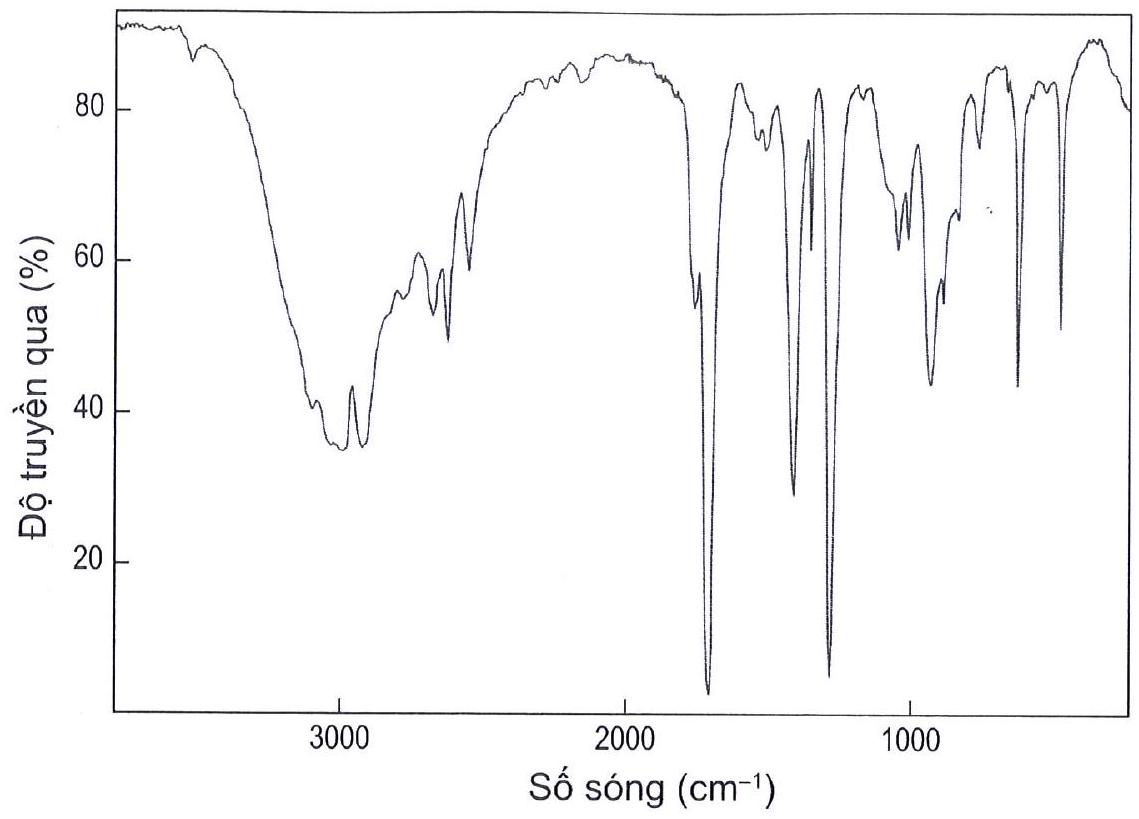
\includegraphics[max width=\textwidth]{2025_10_23_adad5b98d65ac6665838g-01}
\end{center}

\section*{HUODKE DÂN GLÁ}
\section*{Chưong 1. CÂN BẰNG HOÁ HOC}
\section*{Bait}
\section*{1}
\section*{KHÁl NIỆM}
VỀ CÂN BẰNG HOÁ HỌC\\
1.1. Đáp án D.

\section*{1.2. Đáp án D.}
OT6.18. Bạn Nam luôn chăm sóc răng miệng cẩn thận. Vì sợ bị sâu răng nên sau khi ăn cơm, ăn trái cây hay uống nước hoa quả, Nam liền đánh răng ngay. Tuy nhiên, nếu đánh răng ngay sau khi dùng nước trái cây thì sẽ gây hại cho răng. Làm sao để ăn trái cây và uống các loại nước trái cây hằng ngày mà ít gây tác hại nhất cho răng?\\
Em hãy trả lời giúp bạn Nam những vấn đề đặt ra ở trên.\\
OT6.19. Trên thị trường có những lọ măng, dưa chuột muối tuy để lâu nhưng lại không bị hỏng (trong thời hạn sử dụng). Em hãy giải thích lí do.\\
1.3. a) Cân bằng chuyển dịch theo chiều thuận (chiều toả nhiệt).\\
b) Cân bằng chuyển dịch theo chiều thuận (chiều làm giảm nồng độ của khí nitrogen).\\
c) Cân bằng chuyển dịch theo chiều thuận (chiều làm giảm nồng độ của khí hydrogen).\\
d) Cân bằng chuyển dịch theo chiều nghịch (chiều làm tăng áp suất của hệ).\\
1.4. $K_{\mathrm{C}}=\frac{\left[\mathrm{NH}_{3}\right]^{2}}{\left[\mathrm{~N}_{2}\right] \times\left[\mathrm{H}_{2}\right]^{3}}$\\
1.5. $K_{C}=\frac{0,6^{2}}{0,02 \times 2^{3}}=2,25$\\
1.6. a) Cân bằng chuyển dịch theo chiều nghịch (chiều thu nhiệt)\\
b) Cân bằng chuyển dịch theo chiều thuận (chiều làm giảm nồng độ của khí $\mathrm{SO}_{2}$ ).\\
c) Cân bằng chuyển dịch theo chiều thuận (chiều làm giảm nồng độ của khí $\mathrm{O}_{2}$ ).\\
d) Cân bằng chuyển dịch theo chiều thuận (chiều làm tăng nồng độ của $\mathrm{SO}_{3}$ ).\\
1.7. $\mathrm{K}_{\mathrm{C}}=\frac{\left[\mathrm{SO}_{3}\right]^{2}}{\left[\mathrm{O}_{2}\right] \times\left[\mathrm{SO}_{2}\right]^{2}}$\\
1.8.

\begin{center}
\begin{tabular}{lccccc}
 & $2 \mathrm{SO}_{2}(g)$ & $+\mathrm{O}_{2}(g)$ & $\stackrel{\mathrm{V}_{2} \mathrm{O}_{5}, 450^{\circ} \mathrm{C}-500^{\circ} \mathrm{C}}{\sim}$ & $2 \mathrm{SO}_{3}(g)$ &  \\
Ban đầu: & 4 & 2 &  &  & (M) \\
Phản ứng: & 3,2 & 1,6 &  & 3,2 & (M) \\
Cân bằng: & 0,8 & 0,4 &  & 3,2 & (M) \\
\end{tabular}
\end{center}

$$
K_{c}=\frac{3,2^{2}}{0,4 \times 0,8^{2}}=40
$$

1.9. Gọi a là nồng độ oxygen ban đầu cần lấy.

\begin{center}
\begin{tabular}{lcclcl}
 & $2 \mathrm{SO}_{2}(g)+$ & $\mathrm{O}_{2}(g)$ & $\stackrel{\mathrm{V}_{2} \mathrm{O}_{5}, 450^{\circ} \mathrm{C}-500^{\circ} \mathrm{C}}{\Longrightarrow}$ & $2 \mathrm{SO}_{3}(g)$ &  \\
Ban đầu: & 4 & $a$ &  &  & (M) \\
Phản ứng: & 3,6 & 1,8 &  & 3,6 & (M) \\
Cân bằng: & 0,4 & $a-1,8$ &  & 3,6 & (M) \\
\end{tabular}
\end{center}

$$
K_{C}=\frac{3,6^{2}}{(a-1,8) \times 0,4^{2}}=40 \Rightarrow a=3,825(M)
$$

1.10. Cân bằng chuyển dịch theo chiều thuận (chiều làm giảm áp suất của hệ phản ứng).\\
1.11. Đáp án B.\\
1.12. Phản ứng phân huỷ acid HClO làm giảm nồng độ của chất này, cân bằng hoá học của phản ứng xảy ra trong nước chlorine sẽ chuyển dịch theo chiều thuận, chlorine sẽ phản ứng với nước đến khi hết, nên nước chlorine không bảo quản được lâu.\\
1.13. Sự thay đổi áp suất không gây ra sự chuyển dịch cân bằng của mọi phản ứng thuận nghịch. Sự thay đổi áp suất gây ra chuyển dịch cân bằng đối với hệ phản ứng có chất khí, chất lỏng và số mol chất khí, chất lỏng ở hai vế của phương trình hoá học khác nhau.\\
1.14. Hiệu suất lớn nhất: (b), hiệu suất thấp nhất: (a).\\
1.15.

\begin{center}
\begin{tabular}{lcclc}
 & $\mathrm{H}_{2}(\mathrm{~g})+$ & $\mathrm{I}_{2}(\mathrm{~g})$ & $\stackrel{450^{\circ} \mathrm{C}}{\rightleftharpoons}$ & $2 \mathrm{HI}(\mathrm{g})$ \\
Ban đầu: & 1 &  & 1 &  \\
Phản ừng: & 0,78 &  & 0,78 &  \\
Cân bằng: & 0,22 &  & 0,22 &  \\
 &  &  &  & 1,56 \\
 &  &  &  & 1,56 \\
\end{tabular}
\end{center}

$$
\begin{aligned}
& \mathrm{n}_{\mathrm{H}_{2} \text { (phàn ứng) }}=\mathrm{n}_{\mathrm{I}_{2} \text { (phàn ưng) }}=\frac{1,56}{2}=0,78(\mathrm{~mol}) . \\
& \mathrm{n}_{\mathrm{H}_{2} \text { (cón laì) }}=\mathrm{n}_{\mathrm{l}_{2} \text { (còn lại) }}=1-0,78=0,22(\mathrm{~mol}) .
\end{aligned}
$$

Bình có dung tích 1 L , do đó nồng độ mol của chất trong hệ bằng số mol của chất.

$$
K_{c}=\frac{1,56^{2}}{0,22 \times 0,22}=50,28
$$

1.16. $\mathrm{n}_{\mathrm{Cl}_{2}}=\mathrm{n}_{\mathrm{Br}_{2}}=4 \mathrm{~mol} \Rightarrow\left[\mathrm{Br}_{2}\right]=\left[\mathrm{Cl}_{2}\right]=4 \mathrm{M}$.

$$
K_{\mathrm{C}}=\frac{\left[\mathrm{Br}_{2}\right] \times\left[\mathrm{Cl}_{2}\right]}{[\mathrm{BrCl}]^{2}}=11,1 \Rightarrow[\mathrm{BrCl}]=\sqrt{\frac{4 \times 4}{11,1}}=1,2(\mathrm{M}) .
$$

1.17*. Khi thêm dung dịch acid, làm tăng nồng độ ion $\mathrm{H}^{+}$của hệ phản ứng, cân bằng chuyển dịch theo chiều nghịch, hạn chế sự thuỷ phân ion $\mathrm{Fe}^{3+}$ trong dung dịch.\\
1.18*. Dung dịch $\mathrm{H}_{2} \mathrm{SO}_{4}$ đặc có vai trò hút nước, làm cân bằng chuyển dịch theo chiều thuận, làm tăng hiệu suất của phản ứng.\\
1.19*. Phản ứng (4) xảy ra làm giảm nồng độ $\mathrm{H}^{+}$trong hệ phản ứng. Do đó, cân bằng hoá học ở các phản ứng (1), (2) và (3) chuyển dịch theo chiều thuận, tạo thành $\mathrm{Al}(\mathrm{OH})_{3}$ dạng keo màu trắng.\\
1.20*. Trong lòng đại dương có tồn tại cân bằng hoá học:

$$
\mathrm{CaCO}_{3}+\mathrm{H}_{2} \mathrm{O}+\mathrm{CO}_{2} \rightleftharpoons \mathrm{Ca}\left(\mathrm{HCO}_{3}\right)_{2}
$$

Theo nguyên lí chuyển dịch cân bằng, khi nồng độ $\mathrm{CO}_{2}$ tăng thì cân bằng sẽ chuyển dịch theo chiều thuận, làm giảm nồng độ của $\mathrm{CO}_{2}$.\\
Cây xanh và tảo biển quang hợp dưới ánh sáng mặt trời và chất xúc tác là chất diệp lục (chlorophyll) theo phương trình hoá học:

$$
6 \mathrm{CO}_{2}+6 \mathrm{H}_{2} \mathrm{O} \xrightarrow[\text { chorophyll }]{\text { asmt }} \mathrm{C}_{6} \mathrm{H}_{12} \mathrm{O}_{6}+6 \mathrm{O}_{2}
$$

Đây là quá trình tự điều tiết của thiên nhiên, có tác dụng làm chậm quá trình tăng nồng độ $\mathrm{CO}_{2}$ trong khí quyển.

Bai\\
2

\section*{CÂN BẰNG TRONG DUNG DICH NUỚC}
2.1. Đáp án D .\\
2.2. Đáp án B.\\
2.3. Đáp án $B$.\\
2.4. Đáp án $A$.\\
2.5. Đáp án $C$.\\
2.6. Đáp án A .\\
2.7. Đáp án $C$.\\
2.8. Đáp án B .\\
2.9. $\mathrm{NaCl}, \mathrm{KOH}, \mathrm{Ba}(\mathrm{OH})_{2}, \mathrm{AlCl}_{3}, \mathrm{CuSO}_{4}, \mathrm{H}_{2} \mathrm{SO}_{4}$.\\
2.10. $\mathrm{HBr} \rightarrow \mathrm{H}^{+}+\mathrm{Br}^{-}$\\
$\mathrm{HNO}_{3} \rightarrow \mathrm{H}^{+}+\mathrm{NO}_{3}^{-}$\\
$\mathrm{KOH} \rightarrow \mathrm{K}^{+}+\mathrm{OH}^{-}$\\
$\mathrm{Ca}(\mathrm{OH})_{2} \rightarrow \mathrm{Ca}^{2+}+2 \mathrm{OH}^{-}$\\
$\mathrm{Al}_{2}\left(\mathrm{SO}_{4}\right)_{3} \rightarrow 2 \mathrm{Al}^{3+}+3 \mathrm{SO}_{4}^{2-}$\\
$\mathrm{Cu}\left(\mathrm{NO}_{3}\right)_{2} \rightarrow \mathrm{Cu}^{2+}+2 \mathrm{NO}_{3}^{-}$\\
$\mathrm{NaI} \rightarrow \mathrm{Na}^{+}+\mathrm{I}^{-}$\\
$\mathrm{HCN} \rightleftharpoons \mathrm{H}^{+}+\mathrm{CN}^{-}$\\
$\mathrm{HF} \rightleftharpoons \mathrm{H}^{+}+\mathrm{F}^{-}$\\
$\mathrm{HCOOH} \rightleftharpoons \mathrm{H}^{+}+\mathrm{HCOO}^{-}$\\
2.11. a)


\begin{gather*}
\mathrm{Ba}\left(\mathrm{NO}_{3}\right)_{2} \rightarrow \mathrm{Ba}^{2+}+2 \mathrm{NO}_{3}^{-} \\
0,1 \quad 0,1 \quad 0,2 \tag{M}
\end{gather*}


b) $\quad \mathrm{HNO}_{3} \rightarrow \mathrm{H}^{+}+\mathrm{NO}_{3}^{-}$


\begin{gather*}
0,02  \tag{M}\\
\mathrm{KOH} \\
0,02
\end{gathered} \rightarrow \begin{gathered}
0,02 \quad 0,02 \\
\mathrm{~K}^{+}+\mathrm{OH}^{-} \\
0,02 \quad 0,02
\end{gather*}


c)\\
(M)\\
2.12. Nước vôi trong hấp thụ $\mathrm{CO}_{2}$ trong không khí tạo thành $\mathrm{CaCO}_{3}$ và $\mathrm{H}_{2} \mathrm{O}$, làm giảm nồng độ của $\mathrm{Ca}(\mathrm{OH})_{2}$ nên khả năng dẫn điện giảm.\\
2.13. Nước đóng vai trò acid: $\mathrm{b}, \mathrm{d}$.

Nước đóng vai trò base: $\mathrm{a}, \mathrm{c}$.\\
2.14. Acid: HI

Base: $\mathrm{CH}_{3} \mathrm{COO}^{-}, \mathrm{S}^{2-}, \mathrm{PO}_{4}^{3-}, \mathrm{NH}_{3}$

Lưỡng tính: $\mathrm{HPO}_{4}^{2-}, \mathrm{H}_{2} \mathrm{PO}_{4}^{-}$\\
2.15. a) $\mathrm{pH}=-\lg \left(4,2 \times 10^{-10}\right)=9,38$.\\
b) $\left[\mathrm{H}^{+}\right]=10^{-6,35}=4,5 \times 10^{-7}$.\\
c) $\mathrm{pOH}=-\lg \left(4,0 \times 10^{-11}\right) \approx 10,4 \Rightarrow \mathrm{pH}=14-10,4=3,6$.\\
2.16. Gọi $x(L)$ là thể tích nước cần cho vào dung dịch để thực hiện việc pha chế.\\
$\mathrm{pH}=3 \Rightarrow\left[\mathrm{H}^{+}\right]=0,001(\mathrm{M}) \Rightarrow \mathrm{n}_{\mathrm{H}^{+}}=\mathrm{n}_{\mathrm{HCl}}=0,01 \times 0,001=10^{-5}(\mathrm{~mol})$.\\
$\mathrm{pH}=4 \Rightarrow\left[\mathrm{H}^{+}\right]=0,0001(\mathrm{M})=\frac{10^{-5}}{\mathrm{x}+0,01} \Rightarrow \mathrm{x}=0,09(\mathrm{~L})=90(\mathrm{~mL})$.\\
Cách pha: Đong 90 mL nước cất cho từ từ vào bình đựng 10 mL dung dịch HCl có $\mathrm{pH}=3$. Dùng đũa thuỷ tinh khuấy đều.\\
2.17. $\mathrm{HNO}_{3}$ không bền, khi có ánh sáng dễ bị phân huỷ nên không dùng trong chuẩn độ acid - base vì sẽ làm sai lệch kết quả phân tích.\\
2.18. $\mathrm{n}_{\mathrm{H}^{+}(\text {trong } 300 \mathrm{~mL} \text { dung dich } \mathrm{A})}=0,07 \mathrm{~mol}$.

Gọi thể tích dung dịch (B) là $\mathrm{V}_{\mathrm{B}}(\mathrm{L})$ ta có: $\mathrm{n}_{\mathrm{OH}^{-}}=0,2 \mathrm{~V}_{\mathrm{B}}+0,29 \mathrm{~V}_{\mathrm{B}}=0,49 \mathrm{~V}_{\mathrm{B}}$ Khi trộn ( $A$ ) với ( $B$ ) ta có: $\quad \mathrm{H}^{+}+\mathrm{OH}^{-} \rightarrow \mathrm{H}_{2} \mathrm{O}$\\
Dung dịch sau khi trộn có $\mathrm{pH}=2 \Rightarrow\left[\mathrm{H}^{+}\right]=10^{-2}(\mathrm{M})$.

$$
\Rightarrow\left[\mathrm{H}^{+}\right]_{(\mathrm{d} \psi)}=\frac{\left(0,07-0,49 \mathrm{~V}_{\mathrm{B}}\right)}{0,3+\mathrm{V}_{\mathrm{B}}}=10^{-2}=0,01 \Rightarrow \mathrm{~V}_{\mathrm{B}}=0,134(\mathrm{~L}) .
$$

2.19. $[\mathrm{HCl}]=\frac{34 \times 0,12}{40}=0,102(\mathrm{M})$.\\
2.20. $\mathrm{n}_{\mathrm{NaOH}}=0,075 \times 0,05=0,00375(\mathrm{~mol})$.

$$
\begin{array}{lll}
\mathrm{CH}_{3} \mathrm{COOH} & + & \mathrm{NaOH} \rightarrow \mathrm{CH}_{3} \mathrm{COONa}+\mathrm{H}_{2} \mathrm{O} \\
0,00375 & 0,0375 & (\mathrm{~mol})
\end{array}
$$

$$
\left[\mathrm{CH}_{3} \mathrm{COOH}\right]=\frac{0,00375}{0,05}=0,075(\mathrm{M}) .
$$

2.21*.

\begin{itemize}
  \item Đồ thị quá trình chuẩn độ dung dịch HCl bằng dung dịch chuẩn NaOH $0,100 \mathrm{M}$ được trình bày như hình:\\
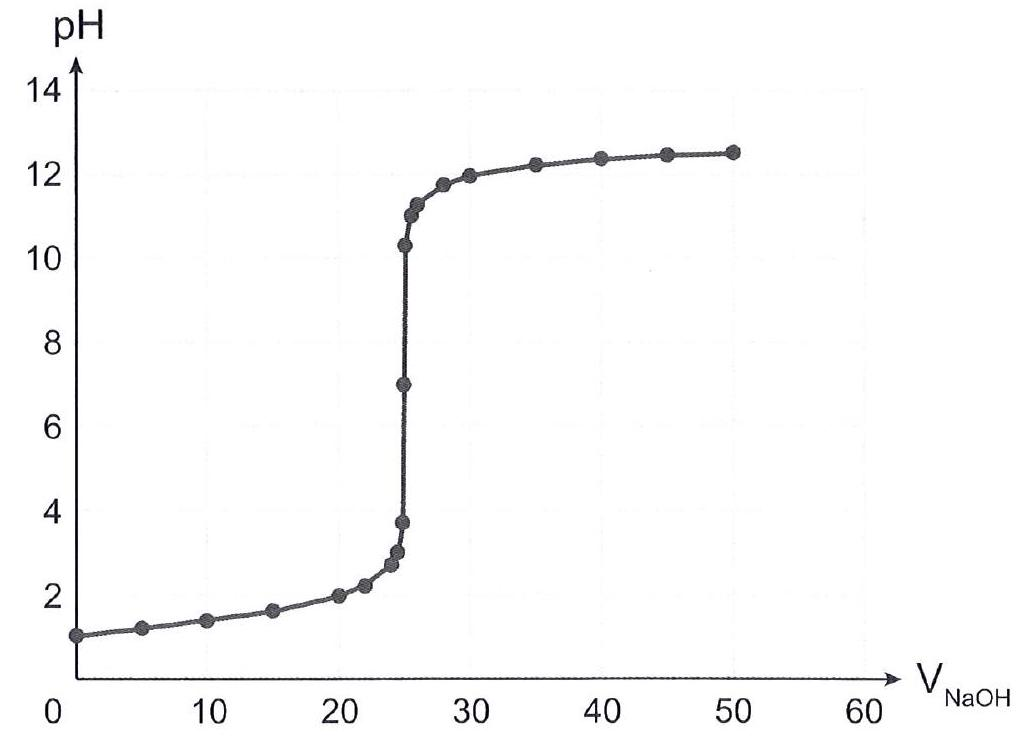
\includegraphics[max width=\textwidth, center]{2025_10_23_adad5b98d65ac6665838g-04}
\end{itemize}

\footnotetext{\begin{itemize}
  \item Điểm tương đương ở $\mathrm{pH}=7$.
  \item Bước nhảy chuẩn độ ở khoảng pH từ 3,7 đến 10,3.
\end{itemize}
}\section*{ÔN TẬP CHƯONG 1}
OT1.1. Đáp án D.\\
OT1.2. Đáp án $C$.\\
OT1.3. Đáp án B.\\
OT1.4. Đáp án A.\\
OT1.5. Đáp án C.\\
OT1.6. $K_{\mathrm{C}}=\frac{0,0387 \times 0,0387}{0,0613 \times 0,1839^{3}}=3,9284$\\
OT1.7. a) chiều thuận; b) chiều nghịch.\\
OT1.8. $K_{C}=\frac{0,150 \times 0,150}{\left[\mathrm{COCl}_{2}\right]}=8,2 \times 10^{-2}$

$$
\Rightarrow\left[\mathrm{COCl}_{2}\right]=0,274(\mathrm{M}) .
$$

OT1.9. $\mathrm{KBr} \rightarrow \mathrm{K}^{+}+\mathrm{Br}^{-}$

$$
\begin{aligned}
& \mathrm{Ca}\left(\mathrm{NO}_{3}\right)_{2} \rightarrow \mathrm{Ca}^{2+}+2 \mathrm{NO}_{3}^{-} \\
& \mathrm{NaOH} \rightarrow \mathrm{Na}^{+}+\mathrm{OH}^{-} \\
& \mathrm{Ba}(\mathrm{OH})_{2} \rightarrow \mathrm{Ba}^{2+}+2 \mathrm{OH}^{-} \\
& \mathrm{Fe}_{2}\left(\mathrm{SO}_{4}\right)_{3} \rightarrow 2 \mathrm{Fe}^{3+}+3 \mathrm{SO}_{4}^{2-} \\
& \mathrm{Zn}\left(\mathrm{NO}_{3}\right)_{2} \rightarrow \mathrm{Zn}^{2+}+2 \mathrm{NO}_{3}^{-} \\
& \mathrm{KI} \rightarrow \mathrm{~K}^{+}+\mathrm{I}^{-} \\
& \mathrm{H}_{2} \mathrm{~S} \rightleftharpoons \mathrm{H}^{+}+\mathrm{HS}^{-} \\
& \mathrm{CH}_{2}=\mathrm{CH}-\mathrm{COOH} \rightleftharpoons \mathrm{H}^{+}+\mathrm{CH}_{2}=\mathrm{CH}-\mathrm{COO}^{-}
\end{aligned}
$$

OT1.10. $\mathrm{n}_{\mathrm{OH}^{-}}=0,01 \mathrm{~V}(\mathrm{~mol}) ; \mathrm{n}_{\mathrm{H}^{+}}=0,03 \mathrm{~V}(\mathrm{~mol})$

$$
\mathrm{H}^{+}+\mathrm{OH}^{-} \rightarrow \mathrm{H}_{2} \mathrm{O}
$$

$\mathrm{n}_{\mathrm{H}^{+}(\mathrm{d} \mathrm{u})}=0,03 \mathrm{~V}-0,01 \mathrm{~V}=0,02 \mathrm{~V}(\mathrm{~mol})$.\\
Nồng độ mol của $\mathrm{H}^{+}$trong dung dịch sau phản ứng $=\frac{0,02 \mathrm{~V}}{2 \mathrm{~V}}=10^{-2}(\mathrm{M})$

$$
\Rightarrow \mathrm{pH}=2 .
$$

\section*{Chuong 2. NLTROESN VA SULFUR}
Brit

\section*{3}
\section*{ĐƠN CHẤT NITROGEN}
3.1. Đáp án A .\\
3.2. Đáp án D .\\
3.3. Đáp án D .\\
3.4. Đáp án A.\\
3.5. a) Nitrogen là phi kim mạnh, nhưng đơn chất nitrogen hoạt động hoá học kém ở nhiệt độ thường, tồn tại được trong tự nhiên (khí quyển) vì phân tử $\mathrm{N}_{2}$ có liên kết ba $(\mathrm{N} \equiv \mathrm{N})$ rất bền, không thể phân huỷ thành nguyên tử khi ở nhiệt độ thấp hoặc không có xúc tác.\\
b) $\mathrm{N}_{2}$ phản ứng với nhiều kim loại (với Li ở nhiệt độ thường và với $\mathrm{Ca}, \mathrm{Mg}$ khi nóng) tạo ra các nitride kim loại ( $\mathrm{Li} \mathrm{N}_{3} \mathrm{~N}, \mathrm{Ca}_{3} \mathrm{~N}_{2}, \mathrm{Mg}_{3} \mathrm{~N}_{2}, \ldots$ ). Khi hình thành Trái Đất, thời kì đầu rất nóng là điều kiện cho nitrogen có thể tạo với một số kim loại mạnh thành những nitride.\\
Nhưng ở nhiệt độ này hydrogen và oxygen cũng đã hoá hợp với nhau tạo thành nước. Khi có mặt nước, các nitride kim loại đều bị thuỷ phân thành base kiềm và ammonia. Ví dụ:

$$
\mathrm{Ca}_{3} \mathrm{~N}_{2}+6 \mathrm{H}_{2} \mathrm{O} \rightarrow 2 \mathrm{NH}_{3}+3 \mathrm{Ca}(\mathrm{OH})_{2}
$$

Ammonia tạo ra có thể cháy, nghĩa là bị oxygen của không khí oxi hoá cho trở lại nitrogen:

$$
4 \mathrm{NH}_{3}+3 \mathrm{O}_{2} \xrightarrow{\mathrm{t}^{\circ}} 2 \mathrm{~N}_{2}+6 \mathrm{H}_{2} \mathrm{O}
$$

Vì các lí do trên nên vỏ Trái Đất không tồn tại các hợp chất nitride.\\
3.6.

$$
\begin{aligned}
& \mathrm{N}_{2}+3 \mathrm{H}_{2} \underset{\mathrm{t}^{\circ}, \mathrm{xt}}{\rightleftharpoons} 2 \mathrm{NH}_{3} \\
& \mathrm{~N}_{2}+\mathrm{O}_{2} \rightleftharpoons 2 \mathrm{NO}
\end{aligned}
$$

3.7. Nồng độ của $\mathrm{N}_{2}$ ban đầu là $\frac{0,5}{0,5}=1(\mathrm{M})$.

Nồng độ của $\mathrm{H}_{2}$ ban đầu là $\frac{1,5}{0,5}=3(\mathrm{M})$.

$$
\Rightarrow\left[\mathrm{NH}_{3}\right]=\frac{0,2}{0,5}=0,4(\mathrm{M}) .
$$

\begin{center}
\begin{tabular}{lcclcl}
 & $\mathrm{N}_{2}(g)+3 \mathrm{H}_{2}(g) \stackrel{\mathrm{t}^{\circ}, \mathrm{xt}}{=}$ & $2 \mathrm{NH}_{3}(g)$ &  &  &  \\
Ban đầu: & 1 & 3 &  &  & (M) \\
Phản ứng: & 0,2 & 0,6 &  & 0,4 & (M) \\
Cân bằng: & 0,8 & 2,4 &  & 0,4 & (M) \\
\end{tabular}
\end{center}

$$
K_{C}=\frac{0,4^{2}}{0,8 \times 2,4^{3}}=0,014
$$

3.8*. Xét phân tử $P_{4}$ : Phân tử $P_{4}$ (phosphorus trắng) là một tứ diện trong đó gồm 4 nguyên tử $P$ chiếm 4 đỉnh, liên kết với nhau bằng 6 liên kết đơn $P-P$.\\
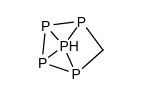
\includegraphics{smile-2b848151a8ab1b324877f516a051bcf80022aa9c}

Bốn nguyên tử P kết hợp với nhau để tạo thành phân tử $\mathrm{P}_{4}$ sẽ giải phóng năng lượng là: $6 \times 209=1254(\mathrm{~kJ})$.\\
Nếu 4 nguyên tử $P$ kết hợp với nhau để tạo thành 2 phân tử $P \equiv P$ thì sẽ giải phóng năng lượng là: $2 \times 490=980(\mathrm{~kJ})$.\\
$\Rightarrow$ Phân tử $P_{4}$ bền hơn $P_{2}$ nên ở điều kiện thường, phosphorus trắng tồn tại ở dạng phân tử $\mathrm{P}_{4}$.\\
Xét phân tử $N_{2}$ : Tính tương tự như trên, năng lượng được giải phóng khi tạo thành một phân tử $\mathrm{N}_{4}$ từ 4 nguyên tử N là: $6 \times 160=960(\mathrm{~kJ})$.\\
Năng lượng được giải phóng khi tạo thành 2 phân tử $\mathrm{N}_{2}$ từ bốn nguyên tử N là: $2 \times 941=1882(\mathrm{~kJ})$.\\
$\Rightarrow$ Phân tử $\mathrm{N}_{2}$ bền hơn $\mathrm{N}_{4}$ ở điều kiện thường.\\
3.9 (1) Quá trình cố định đạm.\\
(2) Quá trình nitrate hoá bởi vi khuẩn.\\
(3) Quá trình hấp thu đạm của rễ cây.\\
(4) Động vật sử dụng thức ăn là thực vật.\\
(5) Động vật chết.\\
(6) Quá trình phân huỷ xác động vật.\\
(7) Quá trình khử nitrogen.

\section*{AMMONIA VÀ MỘT SỐ HỢP CHẤT AMMONIUM}
4.1. Đáp án A .\\
4.2. Đáp án D .\\
4.3. Đáp án B.\\
4.4. Đáp án A.\\
4.5. Đáp án B.\\
4.6. Đáp án B.\\
4.7. Đáp án B.\\
4.8. Đáp án A.\\
4.9. Đáp án B.\\
4.10. Đáp án B.\\
4.11. Ban đầu:

$$
2 \mathrm{NH}_{3}+3 \mathrm{Cl}_{2} \rightarrow \mathrm{~N}_{2}+6 \mathrm{HCl}
$$

Sau đó:

$$
\mathrm{HCl}+\mathrm{NH}_{3} \rightarrow \mathrm{NH}_{4} \mathrm{Cl} \text { (khói trắng) }
$$

4.12. Trong dung dịch ammonia tồn tại cân bằng hoá học sau:

$$
\mathrm{NH}_{3}+\mathrm{H}_{2} \mathrm{O} \rightleftharpoons \mathrm{NH}_{4}^{+}+\mathrm{OH}^{-}
$$

a) Khi đun nóng, màu hồng của dung dịch nhạt dần do khí $\mathrm{NH}_{3}$ bay lên nên làm cân bằng hoá học chuyển dịch theo chiều nghịch, dẫn đến pH của dung dịch giảm xuống (tính base giảm).\\
b) Khi cho HCl vào với số mol bằng số $\mathrm{mol}_{\mathrm{NH}_{3}}$ thì dung dịch mất màu hồng vì tạo ra $\mathrm{NH}_{4} \mathrm{Cl}$ có $\mathrm{pH}<7$.\\
c) Khi thêm một vài giọt dung dịch $\mathrm{Na}_{2} \mathrm{CO}_{3}$, dung dịch (A) có màu hồng đậm vì muối $\mathrm{Na}_{2} \mathrm{CO}_{3}$ thuỷ phân cho môi trường base:

$$
\begin{gathered}
\mathrm{Na}_{2} \mathrm{CO}_{3} \rightarrow 2 \mathrm{Na}^{+}+\mathrm{CO}_{3}^{2-} \\
\mathrm{CO}_{3}^{2-}+\mathrm{H}_{2} \mathrm{O} \rightleftharpoons \mathrm{HCO}_{3}^{-}+\mathrm{OH}^{-}
\end{gathered}
$$

d) Khi thêm $\mathrm{AlCl}_{3}$ tới dư xảy ra phản ứng sau:

$$
\mathrm{AlCl}_{3}+3 \mathrm{NH}_{3}+3 \mathrm{H}_{2} \mathrm{O} \rightarrow \mathrm{Al}(\mathrm{OH})_{3} \downarrow+3 \mathrm{NH}_{4} \mathrm{Cl}
$$

$\mathrm{NH}_{4} \mathrm{Cl}$ và $\mathrm{AlCl}_{3}$ dư đều thuỷ phân cho môi trường acid $\Rightarrow$ màu hồng của dung dịch $(\mathrm{A})$ mất dần.

$$
\begin{gathered}
\mathrm{NH}_{4}^{+}+\mathrm{H}_{2} \mathrm{O} \rightleftharpoons \mathrm{NH}_{3}+\mathrm{H}_{3} \mathrm{O}^{+} \\
\mathrm{Al}^{3+}+3 \mathrm{H}_{2} \mathrm{O} \rightleftharpoons \mathrm{Al}(\mathrm{OH})_{3} \downarrow+3 \mathrm{H}^{+}
\end{gathered}
$$

4.13. a) Khi thêm $\mathrm{H}_{2}$, cân bằng chuyển dịch sang phải. Khi thêm $\mathrm{NH}_{3}$, cân bằng chuyển sang trái.\\
b) Khi tăng thể tích của hệ thì nồng độ của tất cả các chất đều giảm. Cân bằng chuyển dịch sang trái, tức là về phía tạo ra số mol phân tử khí lớn hơn.\\
c) Trong trường hợp a) cũng như b), giá trị hằng số cân bằng $K_{c}$ đều không đổi vì hằng số cân bằng chỉ thay đổi theo nhiệt độ mà ở đây nhiệt độ không đổi.\\
4.14*. $\mathrm{Ca}(\mathrm{OH})_{2} \rightarrow \mathrm{Ca}^{2+}+2 \mathrm{OH}^{-}$\\
$\mathrm{NH}_{4}^{+}+\mathrm{OH}^{-} \rightarrow \mathrm{NH}_{3}+\mathrm{H}_{2} \mathrm{O}$\\
$2 \mathrm{NH}_{3}+3 \mathrm{Cl}_{2} \rightarrow \mathrm{~N}_{2}+6 \mathrm{HCl}$\\
4.15. Biến thiên enthalpy của phản ứng (1) và (2):\\
$\Delta_{\mathrm{r}} \mathrm{H}_{298}^{\mathrm{o}}(1)=(-45,90)+(-134,31)-(-365,61)=185,40(\mathrm{~kJ})$.\\
$\Delta_{\mathrm{r}} \mathrm{H}_{298}^{\mathrm{o}}(2)=82,05+2 \times(-241,82)-(-365,61)=-35,97(\mathrm{~kJ})$.\\
Vì $\Delta_{\mathrm{r}} \mathrm{H}_{298}^{\mathrm{o}}(2)<0 \Rightarrow$ Phản ứng (2) toả nhiệt dễ xảy ra hơn, thực tế phản ứng (1) xảy ra theo chiều ngược lại.\\
4.16. $\mathrm{V}_{\mathrm{O}_{2}}=\frac{841,7 \times 21,03}{100}=177\left(\mathrm{~m}^{3}\right)$.\\
$V_{N_{2}}=\frac{841,7 \times 78,02}{100}=656,7\left(\mathrm{~m}^{3}\right)$.\\
(3) $\Rightarrow \mathrm{V}_{\mathrm{H}_{2}}=3 \times \mathrm{V}_{\mathrm{N}_{2}}=3 \times 656,7=1970\left(\mathrm{~m}^{3}\right)$.\\
(2) $\Rightarrow \mathrm{V}_{\mathrm{CH}_{4}}=\frac{1}{2} \times \mathrm{V}_{\mathrm{O}_{2}}=\frac{177}{2}=88,5\left(\mathrm{~m}^{3}\right)$.\\
$\mathrm{V}_{\mathrm{H}_{2} \mathrm{O}}=\mathrm{V}_{\mathrm{O}_{2}}=177 \mathrm{~m}^{3}$.\\
$(1) \Rightarrow \mathrm{V}_{\mathrm{CH}_{4}}=\frac{1}{4} \times \mathrm{V}_{\mathrm{H}_{2}}=\frac{1}{4} \times 1970=492,5\left(\mathrm{~m}^{3}\right)$.\\
$\mathrm{V}_{\mathrm{H}_{2} \mathrm{O}}=\frac{1}{2} \times \mathrm{V}_{\mathrm{H}_{2}}=\frac{1}{2} \times 1970=985\left(\mathrm{~m}^{3}\right)$.\\
$\Rightarrow \mathrm{V}_{\mathrm{CH}_{4}}=492,5+88,5=581\left(\mathrm{~m}^{3}\right)$.\\
$\mathrm{V}_{\mathrm{H}_{2} \mathrm{O}}=985-177=808\left(\mathrm{~m}^{3}\right)$.\\
4.17. Ammonium nitrate khi ở nhiệt độ cao bị phân huỷ thành khí $\mathrm{N}_{2} \mathrm{O}$ và hơi nước, là một phản ứng toả nhiệt và năng lượng lớn. Khi phản ứng nổ xảy ra, năng lượng được giải phóng một cách đột ngột dưới áp lực rât cao, tăng nhanh, còn được gọi là sóng nổ hoặc sóng xung kích. Sóng xung kích gây ra thiệt hại lớn cho môi trường xung quanh. Ammonium nitrate có thể tự phân huỷ qua thời gian. Tia lửa hàn trong quá trình sửa chữa nhà kho đã khơi mào phản ứng phân huỷ ammonium nitrate gây nổ.

$$
\mathrm{NH}_{4} \mathrm{NO}_{3} \xrightarrow{\mathrm{t}^{\circ}} \mathrm{N}_{2} \mathrm{O}+2 \mathrm{H}_{2} \mathrm{O} \quad \Delta_{\mathrm{r}} \mathrm{H}_{298}^{\circ}=-35,9 \mathrm{~kJ}
$$

\section*{5}
MỘT SỐ HỢP CHẤT VỚI OXYGEN CỦA NITROGEN\\
5.1. Đáp án D.\\
5.2. Đáp án A.\\
5.3. Đáp án $C$.\\
5.4. Đáp án $B$.\\
5.5. Đáp án B.\\
5.6. Có rất nhiều biện pháp để giảm thiểu tác hại của mưa acid, trong đó vấn đề cốt lõi nhất là ý thức của con người. Một số giải pháp có thể kể đên như: - Không sử dụng nước mưa trong sinh hoạt hằng ngày.

\begin{itemize}
  \item Xây dựng quy trình xử lí khí thải.
  \item Kiểm soát lượng khí thải của phương tiện giao thông, phương tiện vận hành bằng động cơ nhằm làm giảm lượng khí thải có chứa các oxide của nitrogen.
  \item Loại bỏ triệt để nitrogen, lưu huỳnh có trong than đá và dầu mỏ trước khi đưa vào sử dụng.
  \item Chuyển sang xu hướng sử dụng các loại năng lượng, nhiên liệu thân thiện với môi trường.
  \item Giáo dục, tuyên truyền nhằm giúp người dân có ý thức hơn trong việc bảo vệ môi trường.\\
5.7. Do nitric acid tinh khiết kém bền, ngay ở điều kiện thường khi có ánh sáng bị phân huỷ một phần.\\
5.8. $4 \mathrm{NH}_{3}+5 \mathrm{O}_{2} \xrightarrow{\mathrm{t}^{\circ}, \mathrm{Pt}} 4 \mathrm{NO}+6 \mathrm{H}_{2} \mathrm{O}$\\
(X)\\
$2 \mathrm{NO}+\mathrm{O}_{2} \rightarrow 2 \mathrm{NO}_{2}$\\
$4 \mathrm{NO}_{2}+\mathrm{O}_{2}+2 \mathrm{H}_{2} \mathrm{O} \rightarrow 4 \mathrm{HNO}_{3}$\\
(Y)
\end{itemize}


\begin{equation*}
\mathrm{N}_{2}+3 \mathrm{H}_{2} \rightleftharpoons \mathrm{to}^{\mathrm{e}, \mathrm{xt}, \mathrm{p}} 2 \mathrm{NH}_{3} \tag{Q}
\end{equation*}


$\mathrm{HNO}_{3}+\mathrm{NH}_{3} \longrightarrow \mathrm{NH}_{4} \mathrm{NO}_{3}$\\
(Z)

\begin{center}
\begin{tabular}{|l|c|}
\multicolumn{1}{|c|}{Tên quá trình} & Thứ tự \\
\hline
Thực vật chết. & $(6)$ \\
\hline
Thiếu oxygen. & $(5)$ \\
\hline
Thiếu ánh sáng mặt trời và oxygen nên tảo, thực vật và cá chết. & $(3)$ \\
\hline
Vi khuẩn phát triển. & $(4)$ \\
\hline
Chất dinh duỡng rửa trôi xuống ao, hồ. & $(1)$ \\
\hline
Tảo nở hoa và thực vật phát triển. & $(2)$ \\
\hline
\end{tabular}
\end{center}

5.10. Xét 100 gam dung dịch $\mathrm{HNO}_{3}$, ta có:\\
$\mathrm{m}_{\mathrm{HNO}_{3}}=60 \% \times 100=60(\mathrm{~g})$.\\
$\mathrm{n}_{\mathrm{HNO}_{3}}=\frac{60}{63}=0,95(\mathrm{~mol})$.\\
$V_{\text {ddHNO }}=\frac{100}{1,41}=70,92(\mathrm{~mL})=0,07092(\mathrm{~L})$.\\
$\left[\mathrm{HNO}_{3}\right]=\frac{0,95}{0,07092}=13,40(\mathrm{M})$.\\
5.11. Các phương trình hoá học:\\
(1) $\mathrm{N}_{2}+\mathrm{O}_{2} \stackrel{3000^{\circ} \mathrm{C}}{\rightleftharpoons} 2 \mathrm{NO}$\\
(2) $2 \mathrm{NO}+\mathrm{O}_{2} \rightarrow 2 \mathrm{NO}_{2}$\\
(3) $4 \mathrm{NO}_{2}+\mathrm{O}_{2}+2 \mathrm{H}_{2} \mathrm{O} \rightarrow 4 \mathrm{HNO}_{3}$\\
(4) $2 \mathrm{HNO}_{3}+\mathrm{CaCO}_{3} \rightarrow \mathrm{Ca}\left(\mathrm{NO}_{3}\right)_{2}+\mathrm{CO}_{2}+\mathrm{H}_{2} \mathrm{O}$\\
(5) $\mathrm{N}_{2}+3 \mathrm{H}_{2} \rightleftharpoons \mathrm{to}, \mathrm{xt}, \mathrm{p} \rightleftharpoons 2 \mathrm{NH}_{3}$\\
(6) $4 \mathrm{NH}_{3}+5 \mathrm{O}_{2} \rightleftharpoons \mathrm{t}^{\circ}, \mathrm{xt} 4 \mathrm{NO}+6 \mathrm{H}_{2} \mathrm{O}$\\
(7) $2 \mathrm{NO}+\mathrm{O}_{2} \rightarrow 2 \mathrm{NO}_{2}$\\
(8) $4 \mathrm{NO}_{2}+\mathrm{O}_{2}+2 \mathrm{H}_{2} \mathrm{O} \rightarrow 4 \mathrm{HNO}_{3}$\\
(9) $\mathrm{HNO}_{3}+\mathrm{NH}_{3} \rightarrow \mathrm{NH}_{4} \mathrm{NO}_{3}$\\
5.12*. a) $\Delta_{\mathrm{r}} \mathrm{H}_{298}^{\circ}=4 \times(-241,82)-(-19,56)-2 \times 50,63=-1048,98(\mathrm{~kJ})$.

Nhiệt đốt cháy 1 kg hỗn hợp lỏng $\left(\mathrm{N}_{2} \mathrm{O}_{4}\right.$ và $\left.\mathrm{N}_{2} \mathrm{H}_{4}\right)$ là:

$$
\frac{1048,98 \times 1000}{(2 \times 32+92)}=6724,23(\mathrm{~kJ}) .
$$

b) Quá trình toả nhiệt mạnh và giải phóng một lượng lớn khí nên hỗn hợp lỏng ( $\mathrm{N}_{2} \mathrm{O}_{4}$ và $\mathrm{N}_{2} \mathrm{H}_{4}$ ) được dùng làm nhiên liệu tên lửa.

Brit\\
6

\section*{SULFUR VÀ SULFUR DIOXIDE}
6.1. Đáp án A .\\
6.2. Đáp án $A$.\\
6.3. Đáp án A .\\
6.4. Đáp án C .\\
6.5. Đáp án C.\\
6.6. Dùng nam châm hút sắt ra khỏi hỗn hợp.\\
6.7. Khối lượng phân tử của lưu huỳnh ở $^{\prime} 900^{\circ} \mathrm{C}$ bằng $2,207 \times 29=64,003(\mathrm{amu})$.

Vậy một phân tử lưu huỳnh gồm $\frac{64,003}{32}=2$ (nguyên tử) lưu huỳnh.\\
$\Rightarrow$ Công thức phân tử của hơi lưu huỳnh ở $900^{\circ} \mathrm{C}$ là $\mathrm{S}_{2}$.\\
6.8. Đốt cháy lưu huỳnh sinh ra khí $\mathrm{SO}_{2}$ độc. Tuy nhiên ở nồng độ thấp, khí này có tác dụng diệt khuẩn. Việc xông khí lưu huỳnh giúp việc bảo quản thuốc không bị mối mọt hay nấm mốc tấn công hoặc hoa quả tươi lâu hơn. Tuy nhiên, trong quá trình xông, lưu huỳnh sẽ lưu lại trên thuốc làm thuốc bị cứng, thay đổi màu sắc, mùi vị. $\mathrm{SO}_{2}$ gặp hơi ẩm trong phổi tạo thành $\mathrm{H}_{2} \mathrm{SO}_{3}$ ảnh hưởng đến phổi và hệ thần kinh, ...

$$
\mathrm{S}+\mathrm{O}_{2} \xrightarrow{\mathrm{t}^{\circ}} \mathrm{SO}_{2}
$$

6.9. Nguồn cung cấp lưu huỳnh tự do chủ yếu là do khai thác từ lòng đất theo phương pháp Frasch. Ngoài ra lưu huỳnh còn được tái chế từ các khí thải độc hại như $\mathrm{SO}_{2}$ (sản phẩm phụ trong công nghiệp luyện kim màu), $\mathrm{H}_{2} \mathrm{~S}$ (được tách từ khí tự nhiên) theo các phản ứng:

$$
\begin{gathered}
2 \mathrm{H}_{2} \mathrm{~S}+\mathrm{O}_{2} \rightarrow 2 \mathrm{~S} \downarrow+2 \mathrm{H}_{2} \mathrm{O} \\
2 \mathrm{H}_{2} \mathrm{~S}+\mathrm{SO}_{2} \rightarrow 3 \mathrm{~S} \downarrow+2 \mathrm{H}_{2} \mathrm{O}
\end{gathered}
$$

6.10. Khi thu hồi thuỷ ngân rơi vãi người ta thường sử dụng bột lưu huỳnh rắc lên những chỗ có thuỷ ngân, vì lưu huỳnh có thể tác dụng với thuỷ ngân tạo thành HgS dạng rắn và không bay hơi:

$$
\mathrm{Hg}+\mathrm{S} \rightarrow \mathrm{HgS}
$$

Khi vô tình làm vỡ nhiệt kế thuỷ ngân trong phòng thí nghiệm, cần rắc ngay bột lưu huỳnh bao phủ tất cả các mảnh vỡ. Sau đó dùng chổi quét sạch, gói vào giấy và cho vào thùng rác.\\
Quá trình thu gom thuỷ ngân cũng đơn giản hơn.\\
6.11. $2 \mathrm{SO}_{2}+\mathrm{O}_{2} \xlongequal{\mathrm{t}^{\circ}, \mathrm{xt}} 2 \mathrm{SO}_{3}$\\
$\mathrm{SO}_{3}+\mathrm{H}_{2} \mathrm{O} \rightarrow \mathrm{H}_{2} \mathrm{SO}_{4}$\\
$\mathrm{Fe}+\mathrm{H}_{2} \mathrm{SO}_{4} \rightarrow \mathrm{FeSO}_{4}+\mathrm{H}_{2}$\\
$\mathrm{CaCO}_{3}+\mathrm{H}_{2} \mathrm{SO}_{4} \rightarrow \mathrm{CaSO}_{4}+\mathrm{CO}_{2}+\mathrm{H}_{2} \mathrm{O}$\\
6.12. Đốt lưu huỳnh sinh ra khí $\mathrm{SO}_{2}$ gây độc cho hệ hô hấp của con người và có thể dẫn đến tử vong. Người dân có thể đối mặt với nguy cơ mưa acid trong khu vực.

$$
\begin{aligned}
& \mathrm{S}+\mathrm{O}_{2} \xrightarrow{\mathrm{t}^{\circ}} \mathrm{SO}_{2} \\
& 2 \mathrm{SO}_{2}+\mathrm{O}_{2} \underset{\mathrm{t}^{\circ}, \mathrm{xt}}{\rightleftharpoons} 2 \mathrm{SO}_{3} \\
& \mathrm{SO}_{3}+\mathrm{H}_{2} \mathrm{O} \rightarrow \mathrm{H}_{2} \mathrm{SO}_{4}
\end{aligned}
$$

6.13*. Phương trình hoá học:

$$
\begin{aligned}
& \mathrm{S}+\mathrm{O}_{2} \xrightarrow{\mathrm{t}^{0}} \mathrm{SO}_{2} \\
& 4 \mathrm{FeS}_{2}+11 \mathrm{O}_{2} \xrightarrow{\mathrm{t}^{0}} 2 \mathrm{Fe}_{2} \mathrm{O}_{3}+8 \mathrm{SO}_{2}
\end{aligned}
$$

\begin{itemize}
  \item Ưu điểm:
\end{itemize}

\begin{itemize}
  \item Là những nguyên liệu có sẵn trong tự nhiên, dễ khai thác.
  \item Không tạo ra sản phẩm phụ tác động đến môi trường.
  \item Phản ứng xảy ra đơn giản, hiệu suất cao.
\end{itemize}

\begin{itemize}
  \item Nhược điểm:
\end{itemize}

\begin{itemize}
  \item Tài nguyên thiên nhiên cạn kiệt.
  \item Quá trình khai thác có thể ảnh hưởng đến hệ sinh thái, môi trường đất xung quanh.\\
6.14. a) Đáp án D.\\
b)
\end{itemize}

\begin{center}
\begin{tabular}{|l|c|c|}
\hline
\multicolumn{1}{|c|}{Giải pháp} & An toàn & Không an toàn \\
\hline
(1) Dùng hoá chất $\mathrm{SO}_{2}$ để bảo quản trái cây &  & $\checkmark$ \\
\hline
(2) Bảo quản trái cây trong tủ lạnh. & $\checkmark$ &  \\
\hline
(3) Kĩ thuật đóng gói bổ sung khí MAP. & $\checkmark$ &  \\
\hline
\end{tabular}
\end{center}

\begin{center}
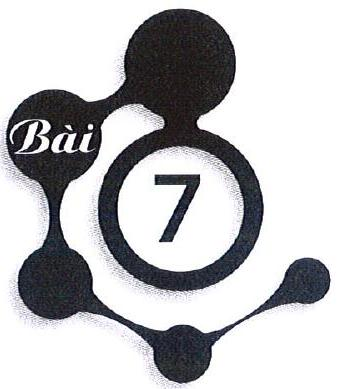
\includegraphics[max width=\textwidth]{2025_10_23_adad5b98d65ac6665838g-09(1)}
\end{center}

\section*{SULFURIC ACID}
VÀ MUỐI SULFATE\\
7.1. Đáp án D.\\
7.2. Đáp án A.\\
7.3. Đáp án B.\\
7.4. Đáp án D.\\
7.5. Đáp án B.\\
7.6. Đáp án B.

Sơ đồ phản ứng:\\
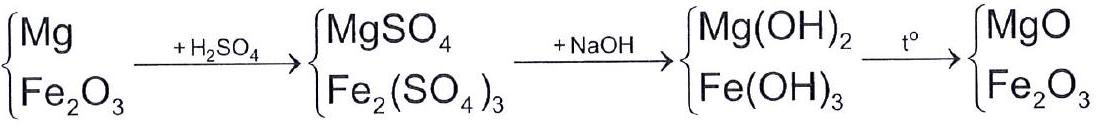
\includegraphics[max width=\textwidth, center]{2025_10_23_adad5b98d65ac6665838g-09}

Vậy khối lượng ban đầu và kết thúc chênh lệch nhau ở khối lượng nguyên tố oxygen của Mg .\\
Theo định luật bảo toàn khối lượng\\
$\Rightarrow \mathrm{m}_{\mathrm{o}}=28-20=8(\mathrm{~g}) \sim 0,5(\mathrm{~mol})$\\
$\Rightarrow \mathrm{m}_{\mathrm{Mg}}=0,5 \times 24=12(\mathrm{~g})$\\
$\Rightarrow \% \mathrm{~m}_{\mathrm{Mg}}=\frac{12}{20} \times 100=60 \%$.\\
7.7. Khối lượng bình tăng lên do $\mathrm{H}_{2} \mathrm{SO}_{4}$ đặc hút nước trong không khí ẩm.\\
7.8.

\begin{center}
\begin{tabular}{|l|l|l|l|}
\hline
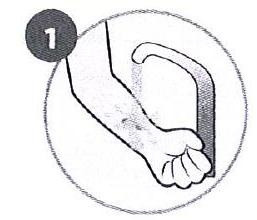
\includegraphics[max width=\textwidth]{2025_10_23_adad5b98d65ac6665838g-10(1)}
 & 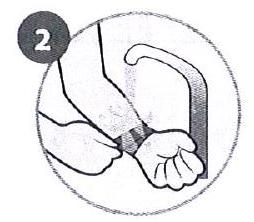
\includegraphics[max width=\textwidth]{2025_10_23_adad5b98d65ac6665838g-10(3)}
 & 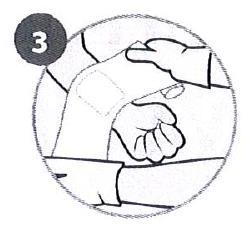
\includegraphics[max width=\textwidth]{2025_10_23_adad5b98d65ac6665838g-10(2)}
 & 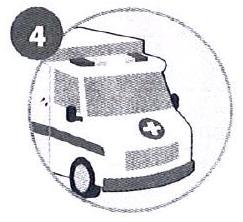
\includegraphics[max width=\textwidth]{2025_10_23_adad5b98d65ac6665838g-10}
 \\
\hline
Cách li nạn nhân ra khỏi acid. Rửa sạch acid trên da dưới vòi nước chảy nhẹ trong ít nhất 20 phút. & Loại bỏ phần trang phục, trang sức dính acid. & Băng vết bỏng bằng băng gạc y tế khô hoặc vải sạch. Có thể dùng các dung dịch trung hoà nhẹ để đắp, tưới rửa vết bỏng. Sau đó, băng ép nhẹ vết bỏng bằng băng sạch. & Nhanh chóng chuyển nạn nhân đến cơ sở y tế gần nhất. Nếu thời gian vận chuyển kéo dài, có thể liên tục tưới rửa vùng bỏng. \\
\hline
\end{tabular}
\end{center}

7.9. Điều kiện phản ứng là: nhiệt độ $450^{\circ} \mathrm{C}-500^{\circ} \mathrm{C}$, xúc tác là vanadium(V) oxide $\left(\mathrm{V}_{2} \mathrm{O}_{5}\right)$.\\
Trong tự nhiên cũng xảy ra quá trình sản xuất sulfuric acid theo các công đoạn trên vì: $\mathrm{SO}_{2}$ là sản phẩm phụ chiếm một lượng lớn trong công nghiệp luyện kim màu, $\mathrm{SO}_{2}$ tiếp tục kết hợp với $\mathrm{O}_{2}$ trong không khí tạo $\mathrm{SO}_{3}$ nhờ chất xúc tác là các oxide kim loại có trong khói bụi khí thải, $\mathrm{SO}_{3}$ kết hợp với nước tạo $\mathrm{H}_{2} \mathrm{SO}_{4}$.\\
7.10. $2 \mathrm{SO}_{2}+\mathrm{O}_{2} \xlongequal{\mathrm{t}^{\circ}, \mathrm{xt}} 2 \mathrm{SO}_{3}$


\begin{equation*}
\mathrm{nSO}_{3}+\mathrm{H}_{2} \mathrm{SO}_{4} \rightarrow \mathrm{H}_{2} \mathrm{SO}_{4} \cdot \mathrm{nSO}_{3} \tag{A}
\end{equation*}



\begin{equation*}
\mathrm{H}_{2} \mathrm{SO}_{4} \cdot \mathrm{nSO}_{3}+\mathrm{nH}_{2} \mathrm{O} \rightarrow(\mathrm{n}+1) \mathrm{H}_{2} \mathrm{SO}_{4} \tag{Q}
\end{equation*}



\begin{equation*}
\mathrm{N}_{2}+3 \mathrm{H}_{2} \stackrel{\mathrm{t}^{0}, \mathrm{xt}}{\rightleftharpoons} 2 \mathrm{NH}_{3} \tag{X}
\end{equation*}


\section*{(Y)}

\begin{equation*}
\mathrm{H}_{2} \mathrm{SO}_{4}+2 \mathrm{NH}_{3} \rightarrow\left(\mathrm{NH}_{4}\right)_{2} \mathrm{SO}_{4} \tag{Z}
\end{equation*}


\begin{table}[h]
\begin{center}
\captionsetup{labelformat=empty}
\caption{7.11. Trích mẫu thử, sử dụng thuốc thử, kết quả thu được theo như bảng:}
\begin{tabular}{|l|l|l|l|l|l|}
\hline
\backslashbox{Thuốc thự}{Mẫu} & $\mathrm{Na}_{2} \mathrm{CO}_{3}$ & $\mathrm{MgSO}_{4}$ & $\mathrm{KNO}_{3}$ & NaOH & HCl \\
\hline
HCl & sủi bọt khí & - & - & - & - \\
\hline
$\mathrm{BaCl}_{2}$ & - & kết tủa trắng & - & - & - \\
\hline
Quỳ tím & - & - & - & xanh & đỏ \\
\hline
\end{tabular}
\end{center}
\end{table}

7.12*. Từ đề bài, ta có: $\mathrm{n}_{\mathrm{Na}_{2} \mathrm{CO}_{3}}=0,15 \mathrm{~mol} ; \mathrm{n}_{\mathrm{CaCO}_{3}}=0,1773 \mathrm{~mol} ; \mathrm{n}_{\mathrm{H}_{2} \mathrm{SO}_{4}}=0,18 \mathrm{~mol}$.

Xét cốc (A): $\mathrm{Na}_{2} \mathrm{CO}_{3}+\mathrm{H}_{2} \mathrm{SO}_{4} \rightarrow \mathrm{Na}_{2} \mathrm{SO}_{4}+\mathrm{CO}_{2} \uparrow+\mathrm{H}_{2} \mathrm{O}$\\
$\mathrm{n}_{\mathrm{H}_{2} \mathrm{SO}_{4}}=0,18>\mathrm{n}_{\mathrm{Na}_{2} \mathrm{CO}_{3}}=0,15 \mathrm{~mol} \Rightarrow \mathrm{H}_{2} \mathrm{SO}_{4}$ du', tính theo $\mathrm{Na}_{2} \mathrm{CO}_{3}$.\\
$\Rightarrow \mathrm{n}_{\mathrm{CO}_{2}}=\mathrm{n}_{\mathrm{Na}_{2} \mathrm{CO}_{3}}=0,15 \mathrm{~mol}$.

Sau phản ứng: $\Delta \mathrm{m}_{\text {cốc } \mathrm{A}}=15,9+18-0,15 \times 44=27,3(\mathrm{~g})$.\\
Xét cốc (B): $2 \mathrm{HCl}+\mathrm{CaCO}_{3} \rightarrow \mathrm{CaCl}_{2}+\mathrm{CO}_{2} \uparrow+\mathrm{H}_{2} \mathrm{O}$\\
Giả thiết nếu $\mathrm{CaCO}_{3} \tan$ hết $\Rightarrow \mathrm{n}_{\mathrm{CO}_{2}}=\mathrm{n}_{\mathrm{CaCO}_{3}}=0,1773$ (mol).\\
$\mathrm{n}_{\mathrm{dd} \mathrm{HCl}} \geq 0,1773 \times 2=0,3546(\mathrm{~mol}) \mathrm{HCl}$.\\
$m_{\text {dd HCl }} \geq \frac{0,3546 \times 36,5}{14,6 \%}=88,65(\mathrm{~g})$.\\
$\Delta \mathrm{m}_{\text {cốc } \mathrm{B}} \geq 17,73+88,65-0,1773 \times 44=98,5788(\mathrm{~g})(>27,3 \mathrm{~g}) \Rightarrow$ Sai với đề, do đó để cân bằng thì $\mathrm{CaCO}_{3}$ phải dư

Đặt số $\mathrm{mol} \mathrm{HCl}=\mathrm{y} \Rightarrow \mathrm{n}_{\mathrm{CO}_{2}}=0,5 \mathrm{y}(\mathrm{mol})$.\\
$m_{d d \mathrm{HCl}}=\frac{y \times 36,5}{14,6 \%}=250 \mathrm{y}(\mathrm{g})$.\\
$\Rightarrow 17,73+250 y-0,5 y \times 44=27,3 \Rightarrow y \approx 0,042(\mathrm{~mol})$.\\
$\Rightarrow m_{d d \mathrm{HCl}}=m=\frac{0,042 \times 36,5}{14,6 \%}=10,49(g)$.\\
7.13*. a) Xét cốc (A): $\quad \mathrm{AgNO}_{3}+\mathrm{HCl} \rightarrow \mathrm{AgCl} \downarrow+\mathrm{HNO}_{3}$

Theo đề ta có: $\mathrm{n}_{\mathrm{AgNO}_{3}}=0,6(\mathrm{~mol})$.\\
$\mathrm{m}_{\mathrm{HCl}}=100 \times 29,2 \%=29,2(\mathrm{~g}) \Rightarrow \mathrm{n}_{\mathrm{HCl}}=0,8(\mathrm{~mol})$.\\
$\mathrm{n}_{\mathrm{HCl}}=0,8>\mathrm{n}_{\mathrm{AgNO}_{3}}=0,6 \Rightarrow \mathrm{HCl}$ du', tính theo $\mathrm{AgNO}_{3}$.\\
$\mathrm{m}_{\mathrm{A} \text { (sau phản ứng) }}=\mathrm{m}_{\mathrm{AgNO}_{3}}+\mathrm{m}_{\mathrm{dd} \mathrm{HCl}}=102+100=202(\mathrm{~g})$.\\
Xét cốc (B): $\quad \mathrm{K}_{2} \mathrm{CO}_{3}+\mathrm{H}_{2} \mathrm{SO}_{4} \rightarrow \mathrm{~K}_{2} \mathrm{SO}_{4}+\mathrm{CO}_{2} \uparrow+\mathrm{H}_{2} \mathrm{O}$\\
Theo đề ta có: $\quad \mathrm{n}_{\mathrm{K}_{2} \mathrm{CO}_{3}}=0,9(\mathrm{~mol})$.

$$
\mathrm{m}_{\mathrm{H}_{2} \mathrm{SO}_{4}}=100 \times 24,5 \%=24,5(\mathrm{~g}) \Rightarrow \mathrm{n}_{\mathrm{H}_{2} \mathrm{SO}_{4}}=0,25(\mathrm{~mol}) .
$$

$\mathrm{n}_{\mathrm{K}_{2} \mathrm{CO}_{3}}=0,9>\mathrm{n}_{\mathrm{H}_{2} \mathrm{SO}_{4}}=0,25 \Rightarrow \mathrm{~K}_{2} \mathrm{CO}_{3} \mathrm{du}$, tính theo $\mathrm{H}_{2} \mathrm{SO}_{4}$.\\
Áp dụng bảo toàn khối lượng:\\
$m_{\mathrm{K}_{2} \mathrm{CO}_{3}}+m_{\mathrm{dd} \mathrm{H}_{2} \mathrm{SO}_{4}}=m_{\mathrm{CO}_{2}}+m_{\text {dung dịch sau phản ứng }}$\\
$\Rightarrow m_{\text {dung dịch sau phản ứng }}=124,2+100-0,25 \times 44=213,2(\mathrm{~g})$.\\
$m_{B}>m_{A} \Rightarrow$ Khối lượng $\mathrm{H}_{2} \mathrm{O}$ thêm vào cốc $(\mathrm{A})=213,2-202=11,2(\mathrm{~g})$.\\
b) Cốc (A) nặng $213,2 \mathrm{~g}$, bao gồm phần rắn $\mathrm{AgCl}(0,6 \times 143,5=86,1 \mathrm{~g})$ và phần dung dịch $(213,2-86,1=127,1 \mathrm{~g})$.\\
$\Rightarrow$ Khối lượng dung dịch $1 / 2$ cốc $(A)=\frac{1}{2} \times 127,1=63,55(\mathrm{~g})$.

Ở $1 / 2$ cốc (A) chứa $0,1 \mathrm{~mol} \mathrm{HCl}$ và $0,3 \mathrm{~mol} \mathrm{HNO}_{3}$ tạo thành.

$$
\begin{array}{rlrl}
\mathrm{HCl} & \rightarrow \mathrm{H}^{+}+\mathrm{Cl}^{-} & \mathrm{HNO}_{3} & \rightarrow \mathrm{H}^{+}+\mathrm{NO}_{3}^{-} \\
0,1 & \rightarrow 0,1 & 0,3 & \rightarrow 0,3
\end{array}
$$

$\mathrm{n}_{\mathrm{H}^{+}}=0,1+0,3=0,4(\mathrm{~mol})$.\\
Ở cốc (B) còn $0,65 \mathrm{~mol} \mathrm{~K}_{2} \mathrm{CO}_{3}$ và $0,25 \mathrm{~mol} \mathrm{~K}_{2} \mathrm{SO}_{4}$ tác dụng với HCl trong cốc (A).

$$
\begin{aligned}
& \mathrm{K}_{2} \mathrm{CO}_{3}+2 \mathrm{HCl} \rightarrow 2 \mathrm{KCl}+\mathrm{CO}_{2} \uparrow+\mathrm{H}_{2} \mathrm{O} \\
& \mathrm{~K}_{2} \mathrm{CO}_{3}+2 \mathrm{HNO}_{3} \rightarrow 2 \mathrm{KNO}_{3}+\mathrm{CO}_{2} \uparrow+\mathrm{H}_{2} \mathrm{O}
\end{aligned}
$$

Hay:

$$
\mathrm{CO}_{3}^{2-}+2 \mathrm{H}^{+} \rightarrow \mathrm{CO}_{2} \uparrow+\mathrm{H}_{2} \mathrm{O}
$$

$\mathrm{n}_{\mathrm{CO}_{2}}=\frac{\mathrm{n}_{\mathrm{H}^{+}}}{2}=0,2(\mathrm{~mol})$.\\
$m_{B \text { sau phản ưng }}=\frac{1}{2} m_{d d A}+m_{d d B}-m_{\mathrm{CO}_{2}}=\frac{1}{2} \times 127,1+213,2-0,2 \times 44=267,95(\mathrm{~g})$. Khối lượng nước thêm vào cốc $(A)=267,95-\left(\frac{1}{2} \times 127,1+86,1\right)=118,3(\mathrm{~g})$.\\
7.14. a)\\
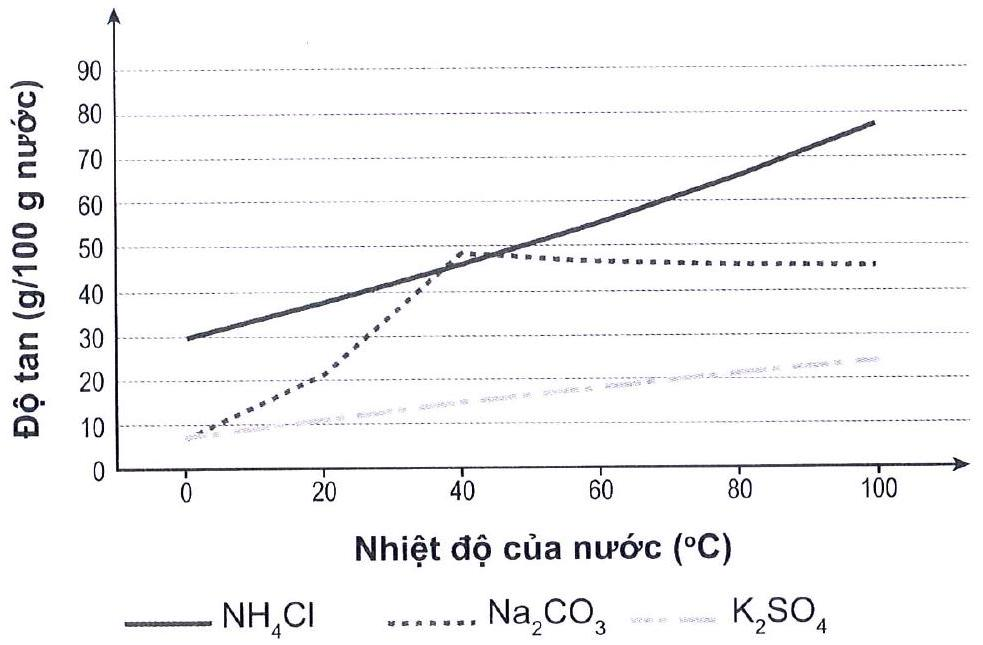
\includegraphics[max width=\textwidth, center]{2025_10_23_adad5b98d65ac6665838g-11}\\
b) Độ tan của các muối tăng theo nhiệt độ. Trong đó, độ tan của $\mathrm{NH}_{4} \mathrm{Cl}$ tăng nhanh, độ tan của $\mathrm{K}_{2} \mathrm{SO}_{4}$ tăng chậm khi nhiệt độ tăng.

Độ tan của muối $\mathrm{Na}_{2} \mathrm{CO}_{3}$ tăng khi nhiệt độ tăng đến khoảng $40^{\circ} \mathrm{C}$. Sau đó độ tan của $\mathrm{Na}_{2} \mathrm{CO}_{3}$ lại bị giảm khi nhiệt độ tăng từ $40^{\circ} \mathrm{C}$ đến $100^{\circ} \mathrm{C}$.

Chất có độ tan lớn nhất là $\mathrm{NH}_{4} \mathrm{Cl}$, ở nhiệt độ $100^{\circ} \mathrm{C}$ có độ tan là $77,30 \mathrm{~g} / 100 \mathrm{~g} \mathrm{H}_{2} \mathrm{O}$.\\
c) Chất có độ tan lớn nhất: ở $30^{\circ} \mathrm{C}$ là $\mathrm{NH}_{4} \mathrm{Cl}$, ở $90^{\circ} \mathrm{C}$ là $\mathrm{NH}_{4} \mathrm{Cl}$.

\section*{ÔN TÂP CHƯONG 2}
OT2.1. Đáp án C.\\
OT2.2. Đáp án A .\\
OT2.3. Đáp án A .\\
OT2.4. Đáp án C .\\
OT2.5. Đáp án B.\\
OT2.6. (D), (C), (B), (A).\\
OT2.7. Sulfuric acid đặc ở nhiệt độ thường không tác dụng với Fe (do Fe bị thụ động hoá bởi $\mathrm{H}_{2} \mathrm{SO}_{4}$ đặc nguội) nên có thể chuyên chở được trong các toa thùng bằng thép. Khi vòi thoát không được đóng kín ngay, sulfuric acid đặc hấp thụ hơi nước trong không khí rất mạnh và trở thành acid loãng sẽ ăn mòn thành toa thùng rất nhanh.

OT2.8. (A) là $\mathrm{N}_{2}$\\
(X) là $\mathrm{H}_{2}$\\
(Y) là $\mathrm{NH}_{3}$\\
$(\mathrm{Z})$ là $\left(\mathrm{NH}_{4}\right)_{2} \mathrm{SO}_{4}$\\
(Q) là $\mathrm{NH}_{4} \mathrm{NO}_{3}$\\
$\mathrm{CH}_{4}+\mathrm{H}_{2} \mathrm{O} \rightarrow \mathrm{CO}+3 \mathrm{H}_{2}$\\
$\mathrm{N}_{2}+3 \mathrm{H}_{2} \xlongequal{\mathrm{t}^{\circ}, \mathrm{xt}} 2 \mathrm{NH}_{3}$\\
$2 \mathrm{NH}_{3}+\mathrm{H}_{2} \mathrm{SO}_{4} \rightarrow\left(\mathrm{NH}_{4}\right)_{2} \mathrm{SO}_{4}$\\
$4 \mathrm{NH}_{3}+5 \mathrm{O}_{2} \xrightarrow{\mathrm{t}^{\circ}, \mathrm{Pt}} 4 \mathrm{NO}+6 \mathrm{H}_{2} \mathrm{O}$\\
$2 \mathrm{NO}+\mathrm{O}_{2} \rightarrow 2 \mathrm{NO}_{2}$\\
$4 \mathrm{NO}_{2}+\mathrm{O}_{2}+2 \mathrm{H}_{2} \mathrm{O} \rightarrow 4 \mathrm{HNO}_{3}$\\
$\mathrm{HNO}_{3}+\mathrm{NH}_{3} \rightarrow \mathrm{NH}_{4} \mathrm{NO}_{3}$\\
OT2.9*. Xét cốc (A):\\
Đặt công thức chung của 2 muối: $\mathrm{RHCO}_{3}$.\\
Giả sử hỗn hợp chỉ có $\mathrm{NaHCO}_{3}$, ta có:\\
$\mathrm{n}_{\mathrm{RHCO}_{3} \text { (lón nhất) }}=\mathrm{n}_{\mathrm{NaHCO}_{3}}=\frac{120}{84} \approx 1,4(\mathrm{~mol})$.\\
$\mathrm{n}_{\mathrm{H}_{2} \mathrm{SO}_{4}}=\frac{100 \times 19,6 \%}{98}=0,2(\mathrm{~mol})$.

$$
2 \mathrm{RHCO}_{3}+\mathrm{H}_{2} \mathrm{SO}_{4} \rightarrow \mathrm{R}_{2} \mathrm{SO}_{4}+2 \mathrm{CO}_{2}+2 \mathrm{H}_{2} \mathrm{O}
$$

Ta có: $\frac{\mathrm{n}_{\mathrm{RHCO}_{3}}}{2}=0,7>\mathrm{n}_{\mathrm{H}_{2} \mathrm{SO}_{4}}=0,2 \Rightarrow \mathrm{RHCO}_{3} \mathrm{du}$, tính theo $\mathrm{H}_{2} \mathrm{SO}_{4}$.\\
$\Rightarrow \mathrm{n}_{\mathrm{CO}_{2}}=0,2 \mathrm{~mol} \Rightarrow \mathrm{~m}_{\mathrm{A}}=120+100-0,2 \times 44=211,2(\mathrm{~g})$.\\
$\Rightarrow \mathrm{n}_{\mathrm{RHCO}_{3} \text { (phản ứng) }}=0,4 \mathrm{~mol} \Rightarrow \mathrm{H}_{2} \mathrm{SO}_{4}$ phản ứng hết.\\
Xét cốc (B): $\mathrm{n}_{\mathrm{AgNO}_{3}}=0,5 \mathrm{~mol} ; \mathrm{n}_{\mathrm{HCl}}=1 \mathrm{~mol}$.

$$
\mathrm{AgNO}_{3}+\mathrm{HCl} \rightarrow \mathrm{AgCl} \downarrow+\mathrm{HNO}_{3}
$$

$\mathrm{n}_{\mathrm{AgNO}_{3}}=0,5<\mathrm{n}_{\mathrm{HCl}}=1 \mathrm{~mol} \Rightarrow \mathrm{HCl}$ du', tính theo $\mathrm{AgNO}_{3}$.\\
$\Rightarrow \mathrm{m}_{\mathrm{B}}=85+100=185(\mathrm{~g}) \Rightarrow$ Hai cốc không thăng bằng.\\
Để cân thăng bằng, cần thêm vào cốc (B): $211,2-185=26,2(\mathrm{~g})$ dung dịch $\mathrm{HCl} 36,5 \%$.

\section*{Chưong 3. ĐAI CUONC HOÁ HOC HÜU CO}
\begin{center}
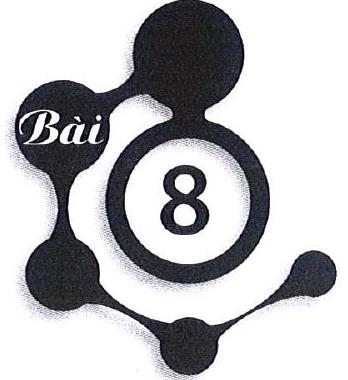
\includegraphics[max width=\textwidth]{2025_10_23_adad5b98d65ac6665838g-13}
\end{center}

\section*{HỢP CHẤT HỮU CƠ VÀ HOÁ HỌC HỮU CO}
8.1. Đáp án B.\\
8.2. Đáp án A .\\
8.3. Đáp án A.\\
8.4. Đáp án C .\\
8.5. Đáp án A .\\
8.6. Chất vô cơ: $\mathrm{NaCl}, \mathrm{H}_{2} \mathrm{SO}_{4}, \mathrm{KOH}, \mathrm{Ba}\left(\mathrm{NO}_{3}\right)_{2}, \mathrm{CO}_{2}, \mathrm{Al}_{4} \mathrm{C}_{3}, \mathrm{KCN}$.

Chất hữu cơ: $\mathrm{CH}_{4}, \mathrm{CH}_{2}=\mathrm{CH}_{2}, \mathrm{HCOONa}, \mathrm{CH}_{3}-\mathrm{CH}_{2}-\mathrm{OH}, \mathrm{CH}_{3}-\mathrm{CH}=\mathrm{O}$.\\
8.7. Hydrocarbon: $\mathrm{CH}_{3}-\mathrm{CH}_{2}-\mathrm{CH}_{3}, \mathrm{CH}_{2}=\mathrm{CH}-\mathrm{CH}_{3}, \mathrm{CH}_{2}=\mathrm{CH}-\mathrm{CH}=\mathrm{CH}_{2}, \mathrm{CH} \equiv \mathrm{CH}$.

Dẫn xuất của hydrocarbon: $\mathrm{CH}_{2}=\mathrm{CH}-\mathrm{COOH}, \mathrm{CH}_{3} \mathrm{OH}, \mathrm{C}_{6} \mathrm{H}_{5} \mathrm{OH}, \mathrm{HCHO}$, $\mathrm{CH}_{3} \mathrm{COOCH}_{3}, \mathrm{H}_{2} \mathrm{~N}-\mathrm{CH}_{2}-\mathrm{COOH}, \mathrm{CH}_{3}-\mathrm{NH}_{2}$.\\
8.8.

\begin{center}
\begin{tabular}{|l|l|}
\hline
\multicolumn{1}{|c|}{Chất hữu cơ} & \multicolumn{1}{c|}{Nhóm chức} \\
\hline
(1) $\mathrm{CH}_{3}-\mathrm{CH}_{2}-\mathrm{OH}$ & -OH \\
\hline
(2) $\mathrm{CH}_{3}-\mathrm{O}-\mathrm{CH}_{2}-\mathrm{CH}_{3}$ & $-\mathrm{O}-$ \\
\hline
(3) $\mathrm{CH}_{3}-\mathrm{CH}_{2}-\mathrm{CH}_{2}-\mathrm{NH}_{2}$ & $-\mathrm{NH}_{2}$ \\
\hline
(4) $\mathrm{CH}_{3}-\mathrm{NH}-\mathrm{CH}_{2}-\mathrm{CH}_{3}$ & $-\mathrm{NH}-$ \\
\hline
(5) $\mathrm{H}-\mathrm{CH}=\mathrm{O}$ & $-\mathrm{CH}=\mathrm{O}$ \\
\hline
(6) $\mathrm{CH}_{3}-\mathrm{CH}_{2}-\mathrm{CH}_{2}-\mathrm{COOH}$ & -COOH \\
\hline
\end{tabular}
\end{center}

8.9. Amine, carboxyl.\\
8.10. Dựa vào phổ IR, nhận thấy peak A ở trong khoảng $3300-3000 \mathrm{~cm}^{-1}$ có sự hiện diện của nhóm -OH. Như vậy, có thể dựa vào peak $A$ giúp dự đoán phổ hồng ngoại này có sự xuất hiện của alcohol trong hợp chất đã nêu.\\
8.11. Dựa vào phổ IR, nhận thấy peak A ở trong khoảng $3300-3000 \mathrm{~cm}^{-1}$ có sự hiện diện của nhóm -OH và peak D khoảng $1700 \mathrm{~cm}^{-1}$ có sự hiện diện của nhóm $\mathrm{C}=\mathrm{O}$. Như vậy, có thể dựa vào peak A và D giúp dự đoán phổ hồng ngoại này có sự xuất hiện của nhóm chức - COOH trong hợp chất đã nêu.\\
8.12. Dựa vào phổ IR, nhận thấy ở vùng $3314 \mathrm{~cm}^{-1}$ có sự hiện diện của nhóm -OH. Như vậy, giúp dự đoán phổ hồng ngoại này tương ứng với hợp chất ethanol.\\
8.13. Dựa vào phổ IR, nhận thấy ở trong khoảng $3300-2500 \mathrm{~cm}^{-1}$ và ở peak $1715 \mathrm{~cm}^{-1}$ có sự hiện diện của nhóm $\mathrm{C}=\mathrm{O}$. Như vậy, dựa vào hai giá trị trên có thể giúp dự đoán hợp chất này có nhóm chức carboxyl trong phân tử.\\
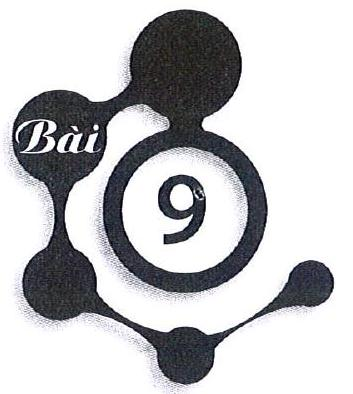
\includegraphics[max width=\textwidth, center]{2025_10_23_adad5b98d65ac6665838g-14}

\section*{PHƯƠNG PHÁP TÁCH VÀ TINH CHẾ HỢP CHẤT HÜU CO}
9.1. Đáp án A .\\
9.2. Đáp án D.\\
9.3. Đáp án C.\\
9.4. Đáp án D.\\
9.5. Đáp án D .\\
9.6. Đáp án A .\\
9.7. Đáp án D .\\
9.8. Đáp án A .\\
9.9. Đáp án A .\\
9.10. Dầu hoả nhẹ hơn nước và không tan trong nước nên hỗn hợp này sẽ tách thành hai lớp. Để tách nước ra khỏi dầu hoả, cho hỗn hợp vào phễu chiết, dầu nổi lên trên và nước ở phía dưới. Mở khoá phễu chiết, nước thoát ra trước sau đó đến dầu hoả, ta được nước và dầu hoả riêng biệt.\\
9.11. Phương pháp chiết: chiết lỏng - rắn (giai đoạn 1) và chiết lỏng - lỏng (giai đoạn 2).\\
9.12. a) Kết tinh; b) Kết tinh; c) Chưng cất.\\
9.13. Kết tinh.\\
9.14. a) Chất a bị hấp phụ mạnh nhất; Chất c bị hấp phụ kém nhất.\\
b) Chất c hoà tan tốt trong dung môi hơn chất a và chất b.\\
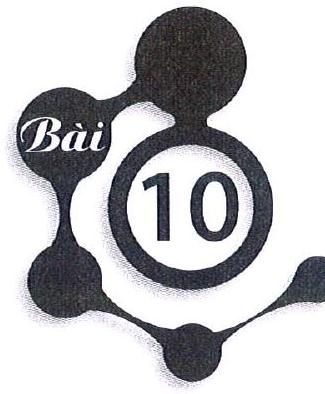
\includegraphics[max width=\textwidth, center]{2025_10_23_adad5b98d65ac6665838g-14(1)}

\section*{CÔNG THỨC PHÂN TỬ HỢP CHẤT HỮU CƠ}
10.1. Ta có: $\% \mathrm{~m}_{\mathrm{c}}=100 \%-7,69 \%=92,31 \%$.

Vì phân tử khối của acetylene gấp 13 lần phân tử khối của hydrogen nên $\mathrm{M}_{\text {Acetylene }}=26$.\\
Acetylene là một hydrocarbon nên có công thức phân tử là $\mathrm{C}_{x} \mathrm{H}_{y}$.

$$
\begin{aligned}
& \frac{12 x}{26}=\frac{92,31}{100} \Rightarrow x \approx 2 \\
& \frac{y}{26}=\frac{7,69}{100} \Rightarrow y \approx 2
\end{aligned}
$$

Công thức phân tử của acetylene là $\mathrm{C}_{2} \mathrm{H}_{2}$.\\
10.2. Dựa trên kết quả phân tích nguyên tố của buta-1,3-diene có $\frac{\% m_{\mathrm{C}}}{\% m_{\mathrm{H}}}=8$\\
nên $\% m_{\mathrm{C}}=88,89 \%$ và $\% m_{\mathrm{H}}=11,11 \%$. nên $\% \mathrm{~m}_{\mathrm{C}}=88,89 \%$ và $\% \mathrm{~m}_{\mathrm{H}}=11,11 \%$.\\
Buta-1,3-diene là một hydrocarbon nên có công thức phân tử là $\mathrm{C}_{\mathrm{x}} \mathrm{H}_{\mathrm{y}}$. Vì phân tử khối của của buta-1,3-diene gấp 1,6875 phân tử khối của oxygen nên $M_{\text {Buta-1,3-diene }}=54$.

$$
\begin{aligned}
& \frac{12 x}{54}=\frac{88,89}{100} \Rightarrow x \approx 4 \\
& \frac{y}{54}=\frac{11,11}{100} \Rightarrow y \approx 6
\end{aligned}
$$

Công thức phân tử của buta-1,3-diene là $\mathrm{C}_{4} \mathrm{H}_{6}$.\\
10.3. Ta có: $\% \mathrm{~m}_{\mathrm{o}}=100 \%-32,00 \%-6,67 \%-18,67 \%=42,66 \%$.

Đặt công thức phân tử của glycine là $\mathrm{C}_{\mathrm{x}} \mathrm{H}_{\mathrm{y}} \mathrm{O}_{\mathrm{z}} \mathrm{N}_{\mathrm{t}}(\mathrm{M}=75)$.

$$
\begin{aligned}
& \frac{12 x}{75}=\frac{32,00}{100} \Rightarrow x=2 \\
& \frac{y}{75}=\frac{6,67}{100} \Rightarrow y \approx 5 \\
& \frac{16 z}{75}=\frac{42,66}{100} \Rightarrow z \approx 2 \\
& \frac{14 t}{75}=\frac{18,67}{100} \Rightarrow t \approx 1
\end{aligned}
$$

Công thức phân tử của glycine là $\mathrm{C}_{2} \mathrm{H}_{5} \mathrm{O}_{2} \mathrm{~N}$.\\
10.4. Dựa trên kết quả phân tích nguyên tố của phenol có $m_{C}: m_{H}: m_{O}=36: 3: 8$ nên $\% m_{C}=76,60 \% ; \% m_{H}=6,38 \%$ và $\% m_{O}=17,02 \%$. Đặt công thức phân tử của phenol là $\mathrm{C}_{\mathrm{x}} \mathrm{H}_{\mathrm{y}} \mathrm{O}_{\mathrm{z}}$.\\
Vì phân tử khối của phenol nặng hơn methane 78 đơn vị nên $\mathrm{M}_{\text {Phenol }}=94$.

$$
\begin{aligned}
& \frac{12 x}{94}=\frac{76,60}{100} \Rightarrow x \approx 6 \\
& \frac{y}{94}=\frac{6,38}{100} \Rightarrow y \approx 6 \\
& \frac{16 z}{94}=\frac{17,02}{100} \Rightarrow z \approx 1
\end{aligned}
$$

Công thức phân tử của phenol là $\mathrm{C}_{6} \mathrm{H}_{6} \mathrm{O}$.\\
10.5. Ta có: $\% m_{N}=100 \%-(37,00 \%+2,20 \%+42,29 \%)=18,51 \%$.

Đặt công thức phân tử của TNT là $\mathrm{C}_{x} \mathrm{H}_{y} \mathrm{O}_{z} \mathrm{~N}_{t}$.\\
Vì phân tử khối của TNT gấp khoảng 2,91 lần phân tử khối của benzene nên $M_{\text {TNT }}=227$.

$$
\begin{aligned}
& \frac{12 x}{227}=\frac{37,00}{100} \Rightarrow x \approx 1 \\
& \frac{y}{227}=\frac{2,20}{100} \Rightarrow y \approx 5
\end{aligned}
$$

$$
\begin{aligned}
& \frac{16 z}{227}=\frac{42,29}{100} \Rightarrow z \approx 6 \\
& \frac{14 t}{227}=\frac{18,51}{100} \Rightarrow t \approx 3
\end{aligned}
$$

Công thức phân tử của TNT là $\mathrm{C}_{7} \mathrm{H}_{5} \mathrm{O}_{6} \mathrm{~N}_{3}$.\\
10.6. Ta có: $\% m_{c}=100 \%-25 \%=75 \%$.\\
$(X)$ là một hydrocarbon nên công thức phân tử của $(X)$ là $C_{x} H_{y}$. Từ phổ khối lượng của $(\mathrm{X})$, suy ra: $\mathrm{M}_{(\mathrm{X})}=16$.

$$
\begin{aligned}
& \frac{12 x}{16}=\frac{75}{100} \Rightarrow x=1 \\
& \frac{y}{16}=\frac{25}{100} \Rightarrow y=4
\end{aligned}
$$

Công thức phân tử của $(\mathrm{X})$ là $\mathrm{CH}_{4}$.\\
10.7. Ta có: $\% \mathrm{~m}_{\mathrm{H}}=100 \%-85,71 \%=14,29 \%$.\\
$(\mathrm{Y})$ là một hydrocarbon nên công thức phân tử của $(\mathrm{Y})$ là $\mathrm{C}_{\mathrm{x}} \mathrm{H}_{\mathrm{y}}$. Từ phổ khối lượng của $(\mathrm{Y})$, suy ra: $\mathrm{M}_{(\mathrm{Y})}=28$.

$$
\begin{aligned}
& \frac{12 x}{28}=\frac{85,71}{100} \Rightarrow x \approx 2 \\
& \frac{y}{28}=\frac{14,29}{100} \Rightarrow y \approx 4
\end{aligned}
$$

Công thức phân tử của $(Y)$ là $\mathrm{C}_{2} \mathrm{H}_{4}$.\\
10.8. $\% \mathrm{~m}_{\mathrm{O}}=100 \%-64,86 \%-13,51 \%=21,63 \%$.

Đặt công thức phân tử của diethyl ether là $\mathrm{C}_{\mathrm{x}} \mathrm{H}_{\mathrm{y}} \mathrm{O}_{\mathrm{z}}$.\\
Từ phổ khối lượng, suy ra: $\mathrm{M}_{\text {Diethyl ether }}=74$.

$$
\begin{aligned}
& \frac{12 x}{74}=\frac{64,86}{100} \Rightarrow x \approx 4 \\
& \frac{y}{74}=\frac{13,51}{100} \Rightarrow y \approx 10
\end{aligned}
$$

$$
\frac{16 z}{74}=\frac{21,63}{100} \Rightarrow z \approx 1
$$

Công thức phân tử của diethyl ether là $\mathrm{C}_{4} \mathrm{H}_{10} \mathrm{O}$.\\
10.9. Dựa trên kết quả phân tích nguyên tố của hợp chất formaldehyde có

$$
\frac{\% \mathrm{H}}{\% \mathrm{O}}=0,125
$$

nên $\% m_{H}=6,67 \% ; \% m_{O}=53,33 \%$.\\
Đặt công thức phân tử của formaldehyde là $\mathrm{C}_{\mathrm{x}} \mathrm{H}_{\mathrm{y}} \mathrm{O}_{\mathrm{z}}$.\\
Từ phổ khối lượng của formaldehyde, suy ra: $\mathrm{M}_{\text {Formaldehyde }}=30$.

$$
\begin{aligned}
& \frac{12 x}{30}=\frac{40}{100} \Rightarrow x=1 \\
& \frac{y}{30}=\frac{6,67}{100} \Rightarrow y \approx 2 \\
& \frac{16 z}{30}=\frac{53,33}{100} \Rightarrow y \approx 1
\end{aligned}
$$

Công thức phân tử của formaldehyde là $\mathrm{CH}_{2} \mathrm{O}$.\\
10.10. $\% m_{H}=100 \%-(26,09 \%+69,57 \%)=4,34 \%$.

Đặt công thức phân tử của formic acid là $\mathrm{C}_{\mathrm{x}} \mathrm{H}_{\mathrm{y}} \mathrm{O}_{\mathrm{z}}$.\\
Từ phổ khối lượng của formic acid, suy ra: $\mathrm{M}_{\text {Formic acid }}=46$.

$$
\begin{aligned}
& \frac{12 x}{46}=\frac{26,09}{100} \Rightarrow x \approx 1 \\
& \frac{y}{46}=\frac{4,34}{100} \Rightarrow y \approx 2 \\
& \frac{16 z}{46}=\frac{69,57}{100} \Rightarrow z \approx 2
\end{aligned}
$$

Công thức phân tử của formic acid là $\mathrm{CH}_{2} \mathrm{O}_{2}$.\\
10.11. $M_{(A)}=28=14 n \Rightarrow n=2 \Rightarrow$ Công thức phân tử của $(A)$ là $C_{2} H_{4}$.\\
$M_{(B)}=42=14 n \Rightarrow n=3 \Rightarrow$ Công thức phân tử của (B) là $C_{3} H_{6}$.\\
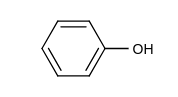
\includegraphics{smile-ea6ef1ff42c3b60b097705893ab495201362acec}

(B)

\section*{(3ad 11 CẤU TẠO HOÁ HỌC HỢP CHẤT HỮU CƠ}
11.1. Đáp án $C$.\\
11.2. Đáp án C.\\
11.3. Đáp án D.\\
11.4. Đáp án $C$.\\
11.5. Mạch hở, không nhánh: $(A)$, ( $E$ ).

Mạch hở, có nhánh: (C), (B).\\
Mạch vòng: (D), (G).\\
11.6. (A) $\mathrm{CH} \equiv \mathrm{C}-\mathrm{CH}=\mathrm{CH}_{2}$.\\
(B) $\mathrm{CH}_{2} \mathrm{OH}-\mathrm{CHOH}-\mathrm{CHOH}-\mathrm{CHOH}-\mathrm{CHOH}-\mathrm{CH}=\mathrm{O}$.\\
(C) $\mathrm{CH}_{3}-\mathrm{CH}\left(\mathrm{NH}_{2}\right)-\mathrm{COOH}$.\\
(D)\\
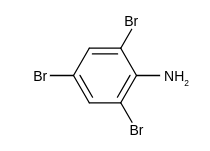
\includegraphics{smile-f3b1234615d12f663786c365593897ff9d753c99}\\
11.7.\\
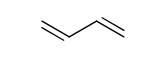
\includegraphics{smile-fdbdfc37788b86bf80b92f403c7bdc96158cf576}\\
(C)\\
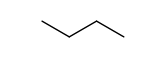
\includegraphics{smile-52329a4ab613d07648b2a21cb02106034622a52a}\\
(D)\\
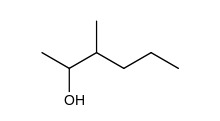
\includegraphics{smile-f9c254597879354a187d4de95414d11aa0118f37}\\
(E)\\
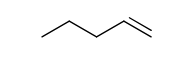
\includegraphics{smile-9d627bcfff33cccb48fd6d316a6416a1199c8658}\\
(G)\\
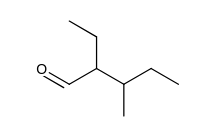
\includegraphics{smile-22ea30964e8bf9756091af8f77e7fb0c298d0b96}\\
(H)\\
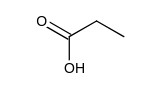
\includegraphics{smile-89e9294cfa4d3f3a56e515c80a45e3c5952c0a00}\\
(I)\\
11.8. Bài 11.6: (A) $\mathrm{C}_{4} \mathrm{H}_{4}$; (B) $\mathrm{C}_{6} \mathrm{H}_{12} \mathrm{O}_{6}$; (C) $\mathrm{C}_{3} \mathrm{H}_{7} \mathrm{O}_{2} \mathrm{~N}$; (D) $\mathrm{C}_{6} \mathrm{H}_{4} \mathrm{Br}_{3} \mathrm{~N}$.\\
Bài 11.7: (A) $\mathrm{C}_{8} \mathrm{H}_{8}$;\\
(B) $\mathrm{C}_{6} \mathrm{H}_{6} \mathrm{O}$;\\
(C) $\mathrm{C}_{4} \mathrm{H}_{6}$;\\
(D) $\mathrm{C}_{3} \mathrm{H}_{8}$;\\
(E) $\mathrm{C}_{5} \mathrm{H}_{12} \mathrm{O} ;(\mathrm{G}) \mathrm{C}_{4} \mathrm{H}_{8} ;$ (H) $\mathrm{C}_{8} \mathrm{H}_{16} \mathrm{O}$; (I) $\mathrm{C}_{3} \mathrm{H}_{6} \mathrm{O}_{2}$.\\
11.9. (a), (b), (c), (d), (e), (g) là những chất thuộc dãy đồng đẳng của $\mathrm{CH}_{3} \mathrm{OH}$.\\
11.10. $\mathrm{CH}_{3} \mathrm{CH}_{2} \mathrm{COOH}$ và $\mathrm{CH}_{3} \mathrm{COOCH}_{3}$. Vì 2 chất đều có công thức phân tử là $\mathrm{C}_{3} \mathrm{H}_{6} \mathrm{O}_{2}$.\\
11.11.\\
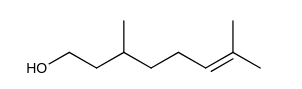
\includegraphics{smile-2d9f54d35a28631be43d8155f8b18cbad0ef85fc}

\section*{ÔN TẬP CHƯONG 3}
OT3.1. Đáp án A.\\
OT3.2. Đáp án B.\\
OT3.3. Đáp án C.\\
OT3.4. Đáp án A.\\
OT3.5. Đáp án A .\\
OT3.6. Chất vô cơ: $\mathrm{AlCl}_{3}, \mathrm{HNO}_{3}, \mathrm{Ba}(\mathrm{OH})_{2}, \mathrm{Na}_{2} \mathrm{CO}_{3}, \mathrm{CO}, \mathrm{CaC}_{2}, \mathrm{NaCN}$.\\
Chất hữu cơ: $\mathrm{CH}_{3}-\mathrm{CH}_{2}-\mathrm{CH}_{3}, \mathrm{CH}_{2}=\mathrm{CH}-\mathrm{CH}_{2}-\mathrm{CH}_{3}, \mathrm{NaOOC}-\mathrm{COONa}$, $\mathrm{CH}_{2} \mathrm{OH}-\mathrm{CH}_{2} \mathrm{OH}, \mathrm{H}-\mathrm{CH}=\mathrm{O}$.\\
OT3.7. Hydrocarbon: $\mathrm{CH}_{4}, \mathrm{CH}_{2}=\mathrm{CH}_{2}, \mathrm{CH}_{2}=\mathrm{CH}\left(\mathrm{CH}_{3}\right)-\mathrm{CH}=\mathrm{CH}_{2}, \mathrm{CH} \equiv \mathrm{CH}$.\\
Dẫn xuất của hydrocarbon: $\mathrm{CH}_{3}-\mathrm{CH}_{2}-\mathrm{NH}_{2}, \mathrm{CH}_{3}-\mathrm{COOH}, \mathrm{C}_{3} \mathrm{H}_{5}(\mathrm{OH})_{3}$, $\mathrm{C}_{6} \mathrm{H}_{5} \mathrm{OH}, \mathrm{CH}_{3} \mathrm{CHO}, \mathrm{CH}_{3} \mathrm{COOCH}_{2} \mathrm{CH}_{3}, \mathrm{H}_{2} \mathrm{~N}-\mathrm{CH}\left(\mathrm{CH}_{3}\right)-\mathrm{COOH}$.\\
OT3.8. Giai đoạn 3: phương pháp chưng cất; giai đoạn 4: phương pháp chiết.\\
OT3.9. Dựa vào phổ IR, nhận thấy peak A ở trong khoảng $3300-3000 \mathrm{~cm}^{-1}$ có sự hiện diện của nhóm -OH. Như vậy, có thể dựa vào peak A giúp dự đoán phổ hồng ngoại này có sự xuất hiện của nhóm - OH trong hợp chất glycerol đã nêu.\\
OT3.10. $\% \mathrm{~m}_{\mathrm{H}}=100 \%-93,75 \%=6,25 \%$.\\
Naphthalene là một hydrocarbon nên có công thức phân tử là $\mathrm{C}_{\mathrm{x}} \mathrm{H}_{\mathrm{y}}$. Từ phổ khối lượng, suy ra: $\mathrm{M}_{\text {Naphthalene }}=128$.

$$
\frac{12 x}{128}=\frac{93,75}{100} \Rightarrow x=10 ; \quad \frac{y}{128}=\frac{6,25}{100} \Rightarrow y=8
$$

Công thức phân tử của naphthalene là $\mathrm{C}_{10} \mathrm{H}_{8}$.\\
OT3.11. a) $\% \mathrm{~m}_{\mathrm{H}}=100 \%-40 \%-53,33 \%=6,67 \%$.\\
Đặt công thức phân tử của acetic acid là $\mathrm{C}_{x} \mathrm{H}_{y} \mathrm{O}_{z}$.\\
Từ phổ khối lượng, suy ra: $\mathrm{M}_{\text {Acetic acid }}=60$.\\
$\frac{12 x}{60}=\frac{40}{100} \Rightarrow x=2 ; \quad \frac{y}{60}=\frac{6,67}{100} \Rightarrow y \approx 4 ; \quad \frac{16 z}{60}=\frac{53,33}{100} \Rightarrow z \approx 2$.\\
Công thức phân tử của acetic acid là $\mathrm{C}_{2} \mathrm{H}_{4} \mathrm{O}_{2}$.\\
b) Dựa vào phổ IR, nhận thấy peak A ở trong khoảng $3300-3000 \mathrm{~cm}^{-1}$ có sự hiện diện của nhóm - OH và peak C trong khoảng $1700 \mathrm{~cm}^{-1}$ có sự hiện diện của nhóm $\mathrm{C}=\mathrm{O}$. Như vậy, có thể dựa vào peak A và D giúp dự đoán phổ hồng ngoại này có sự xuất hiện của nhóm chức - COOH trong hợp chất đã nêu.

\section*{Chuong 4. HYDROCARBON}
\begin{center}
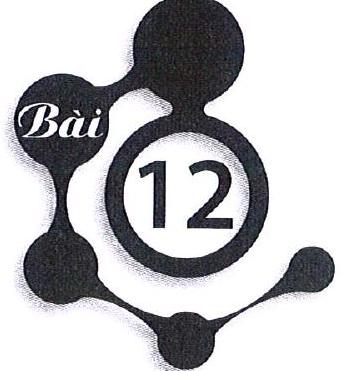
\includegraphics[max width=\textwidth]{2025_10_23_adad5b98d65ac6665838g-18}
\end{center}

\section*{ALKANE}
12.1. Đáp án $C$.\\
12.2. Đáp án $C$.\\
12.3. Đáp án A . Theo đồ thị, có 4 alkane (số nguyên tử carbon từ 1 đến 4) đều có nhiệt độ sôi thấp hơn nhiệt độ phòng nên chúng sẽ ở thể khí trong điều kiện thường.\\
12.4. Đáp án $C$.\\
12.5. Đáp án A. Có methane, ethane và 2,2 -dimethylpentane khi tác dụng với chlorine (có ánh sáng hoặc đun nóng) tạo duy nhất một sản phẩm thế monochloro.\\
12.6. Đáp án A .\\
12.7. Đáp án D.\\
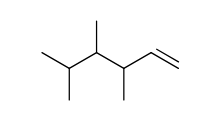
\includegraphics{smile-40126ffb2780a7e1387cff9609c8288e60339d29}

2,3-dimethylpentane

Lưuý:\\
A. 2-ethyl-3-methylbutane: Sai vì mạch chính có 5 nguyên tử carbon, không phải 4 nguyên tử carbon.\\
B. 2-methyl-3-ethylbutane: Sai vì mạch chính có 5 nguyên tử carbon, không phải 4 nguyên tử carbon.\\
C. 3,4-dimethylpentane: Sai vì tổng chỉ số các nhánh lớn hơn so với tên gọi đúng đã nêu.\\
12.8. Chú ý chuỗi 4 nguyên tử carbon chỉ chứa liên kết đơn có thể được "bẻ" theo nhiều cách khác nhau vì các liên kết $\mathrm{C}-\mathrm{C}$ có thể quay tự do. Tuy nhiên, có 7 cách quay các liên kết $\mathrm{C}-\mathrm{C}$ trong hình mà vẫn không làm thay đổi bản chất giữa chúng. Do đó thực chất $\mathrm{C}_{4} \mathrm{H}_{10}$ chỉ có 2 đồng phân.\\
12.9. Các phân tử alkane phân nhánh có nhiệt độ sôi thấp hơn các phân tử alkane không phân nhánh dù cho chúng có cùng số nguyên tử carbon. Điều này được giải thích vì các phân tử alkane không phân nhánh có diện tích bề mặt lớn hơn so với phân tử alkane phân nhánh nên tồn tại tương tác van der Waals giữa các phân tử lớn hơn, dẫn đến nhiệt độ sôi cao hơn.\\
12.10. Trong số 3 đồng phân của $\mathrm{C}_{5} \mathrm{H}_{12}$, neopentane có cấu trúc đối xứng cao, phân tử xem như có dạng hình cầu nên tương tác van der Waals giữa các phân tử neopentane rất yếu, dẫn đến nhiệt độ sôi của neopentane là $9,5^{\circ} \mathrm{C}$. Điều này làm cho phân tử neopentane ở thể khí trong điều kiện thường (hai đồng phân còn lại là pentane có nhiệt độ sôi ở $36^{\circ} \mathrm{C}$ và isopentane có nhiệt độ sôi ở $27,8^{\circ} \mathrm{C}$ nên trong điều kiện thường, chúng ở thể lỏng).\\
12.11. Xăng có thành phần chính là các phân tử alkane có số nguyên tử carbon từ $7-11$ nguyên tử. Vì xăng là các phân tử không phân cực trong khi nước là phân tử phân cực, nên xăng không tan được trong nước. Đồng thời, chất béo là hợp chất không phân cực nên chất béo cũng tan được trong xăng. Dầu mỡ sửa chữa xe cũng là các phân tử alkane nên không thể tan được trong nước, điều đó được hiểu là dầu mỡ trên tay bác thợ sửa chữa xe không thể làm sạch chỉ bởi nước. Bác thợ sửa xe thường dùng dầu hoả (là các phân tử alkane có số nguyên tử carbon từ $12-15$ nguyên tử) để hoà tan các vết dầu mỡ, sau đó rửa lại bằng xà phòng.\\
12.12. Khi tiếp xúc lâu dài với xăng, dầu hoả, ... sẽ làm cho lớp dầu bảo vệ da bị trôi đi, da không còn lớp dầu bảo vệ nên sẽ bị phồng rộp và gây đau nhức. Vì vậy khi tiếp xúc với xăng, dầu hoả, dung môi pha sơn, ... cần đeo găng tay cẩn thận.\\
12.13. Butane là chất lỏng có thể nhìn thấy bên trong một chiếc bật lửa trong suốt, có nhiệt độ sôi thấp hơn một ít so với nhiệt độ của nước đóng băng ( $-0,5^{\circ} \mathrm{C}$ ). Tuy nhiên butane trong bật lửa lại không sôi. Điều này được giải thích là do khi được đưa vào trong bật lửa, butane chịu áp suất rất cao so với áp suất khí quyển, việc tăng áp suất này đã làm cho các phân tử khí butane\\
"lại gần nhau hơn" và "bị ép" thành thể lỏng. Vì vậy butane trong bật lửa được nén và lưu lại dưới dạng lỏng. Khi được giải nén, chất lỏng lập tức bốc hơi và tạo khí butane, bốc cháy khi gặp tia lửa do ma sát giữa bánh răng kim loại với đá lửa.\\
12.14. Do 2 -methylpropane có 3 nhóm $-\mathrm{CH}_{3}$ có vị trí tương tự nhau nên chỉ có\\
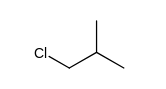
\includegraphics{smile-6bd4d6fca35d0608bc28b02ad31cb1fc467e6eb3}

1-chloro-2-methylpropane\\
2 sản phẩm thế monochloro tạo thành sau phản ứng là:\\
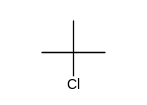
\includegraphics{smile-755a8cffea9f04219d628804b192030067108245}

2-chloro-2-methylpropane\\
12.15. 2-methylpropane có công thức cấu tạo:\\
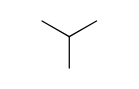
\includegraphics{smile-5ed9796ff9dd905ff370aa0b6fb1b93fb339d590}

Như vậy 2-methylpropane có 9 nguyên tử hydrogen gắn ở nguyên tử carbon bậc I và 1 nguyên tử hydrogen gắn ở nguyên tử carbon bậc III. Gọi a và ka là khả năng phản ứng tương đối của nguyên tử hydrogen gắn ở nguyên tử carbon bậc I và nguyên tử carbon bậc III trong phản ứng thế bromine đã cho, ta có phương trình:

$$
\frac{9 a \times 100}{9 a+k a}=0,56 \Leftrightarrow k=1598
$$

Vậy với 2-methylpropane, tỉ lệ khả năng phản ứng tương đối của nguyên tử hydrogen gắn ở nguyên tử carbon bậc I và nguyên tử carbon bậc III trong phản ứng là $1: 1598$. Điêu này đã cho thấy trong phản ứng thế halogen, bromine thể hiện tính chọn lọc cao hơn nhiều so với chlorine (ở phản ứng với chlorine, tỉ lệ này của 2 -methylpropane là $1: 5$ ).\\
12.16. a) Propane $\mathrm{CH}_{3}-\mathrm{CH}_{2}-\mathrm{CH}_{3}$ có 6 nguyên tử hydrogen gắn ở carbon bậc I và 2 nguyên tử hydrogen gắn ở carbon bậc II. Khi tác dụng với chlorine sẽ thu được 2 sản phẩm thế monochloro là $\mathrm{CH}_{3}-\mathrm{CH}_{2}-\mathrm{CH}_{2} \mathrm{Cl}$ và $\mathrm{CH}_{3}-\mathrm{CHCl}-\mathrm{CH}_{3}$. Tổng khả năng phản ứng của 8 nguyên tử hydrogen là $6 \times 1+4 \times 2=14$. Do 6 nguyên tử hydrogen ở nguyên tử carbon bậc I đều có khả năng phản ứng như nhau để tạo sản phẩm $\mathrm{CH}_{3}-\mathrm{CH}_{2}-\mathrm{CH}_{2} \mathrm{Cl}$ nên khả năng tạo $\mathrm{CH}_{3}-\mathrm{CH}_{2}-\mathrm{CH}_{2} \mathrm{Cl}$ là $\frac{6 \times 100}{14}=42,85 \%$.

Ngoài ra, 2 nguyên tử hydrogen gắn ở nguyên tử carbon bậc II đều có khả năng phản ứng như nhau để tạo sản phẩm $\mathrm{CH}_{3}-\mathrm{CHCl}-\mathrm{CH}_{3}$ nên khả năng tạo $\mathrm{CH}_{3}-\mathrm{CHCl}-\mathrm{CH}_{3}$ là $\frac{2 \times 4}{14} \times 100=57,15 \%$.\\
b) Phản ứng của propane với bromine sẽ xảy ra chậm hơn so với phản ứng của propane với chlorine. Tuy nhiên lúc này, do bromine có tính chọn lọc hơn so với chlorine nên khả năng phản ứng của nguyên tử carbon bậc II cao hơn nhiều so với của nguyên tử carbon bậc I , dẫn đến sản phẩm thế $\mathrm{CH}_{3}-\mathrm{CHBr}-\mathrm{CH}_{3}$ sẽ cao hơn nhiều so với sản phẩm thế $\mathrm{CH}_{3}-\mathrm{CH}_{2}-\mathrm{CH}_{2} \mathrm{Br}$.\\
12.17. Lớp nhũ màu trắng bạc phản xạ tốt các tia nhiệt, có nghĩa là hấp thụ các tia nhiệt kém nên hạn chế được sự truyền nhiệt từ bên ngoài vào, nhờ đó xăng đỡ nóng hơn, tránh hiện tượng gây cháy nổ bể.\\
12.18. a) Vi $\% \mathrm{~m}_{\mathrm{C}}+\% \mathrm{~m}_{\mathrm{H}}=100 \%$ nên phân tử $(\mathrm{X})$ chỉ chứa các nguyên tố hydrogen và carbon.\\
Đặt công thức phân tử của $(X)$ là $C_{x} H_{y}$, ta có:

$$
x: y=\frac{\% C}{12}: \frac{\% H}{1}=\frac{84,21}{12}: \frac{15,79}{1}=7,0175: 15,79=4: 9
$$

Vậy công thức phân tử của $(X)$ có dạng $\left(\mathrm{C}_{4} \mathrm{H}_{9}\right)_{n}$. Phổ khối lượng của $(X)$ cho thấy $(X)$ có phân tử khối là 114 .\\
$M_{(x)}=114 \Leftrightarrow 57 n=114 \Rightarrow n=2$.\\
Do đó công thức phân tử của $(X)$ là $\mathrm{C}_{8} \mathrm{H}_{18}$.\\
b) Công thức phân tử $(X)$ có dạng $\left(\mathrm{C}_{4} \mathrm{H}_{9}\right)_{n}$ hay $\mathrm{C}_{4 n} \mathrm{H}_{9 n}$.

Trong hợp chất $\mathrm{C}_{\mathrm{x}} \mathrm{H}_{\mathrm{y}} \mathrm{O}_{\mathrm{z}}$ bất kì, ta phải có $\mathrm{y} \leq 2 \mathrm{x}+2$ nên $9 \mathrm{n} \leq 2 \times 4 \mathrm{n}+2 \Rightarrow \mathrm{n} \leq 2$.\\
Với giá trị $\mathrm{n}=1$ cho ( X ) có công thức $\mathrm{C}_{4} \mathrm{H}_{9}$. Điều này không hợp lí vì hợp chất chứa $\mathrm{C}, \mathrm{H}$ hoặc $\mathrm{C}, \mathrm{H}, \mathrm{O}$ phải có số nguyên tử hydrogen là số chẵn. Vậy công thức phân tử $(X)$ là $\mathrm{C}_{8} \mathrm{H}_{18}$.

Hoặc: Do $(X)$ có phân tử khối là 114 nên $(X)$ có công thức phân tử $\mathrm{C}_{8} \mathrm{H}_{18}$ hoặc $\mathrm{C}_{9} \mathrm{H}_{6}$. Nhưng hợp chất $\mathrm{C}_{9} \mathrm{H}_{6}$ có $\% \mathrm{~m}_{\mathrm{C}}=94,74 \%$, loại vì sai với dữ kiện đề bài. Vậy $(X)$ có công thức phân tử là $C_{8} H_{18}$.\\
12.19*. Đánh số trên mạch chính là mạch dài nhất:\\
a)\\
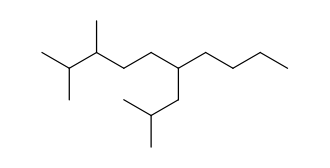
\includegraphics{smile-c05ff8a8f6a902df806937c71558d014007dd2a0}

6-isobutyl-2,3-dimethyldecane

hay 2,3-dimethyl-6-(2-methylpropyl)decane

Ở đây, ở vị trí carbon số 6 có nhánh phức tạp. Để đọc tên nhánh này, carbon của nhánh phức tạp gắn vào mạch chính được đánh số 1 (xem hình). Tên nhánh phức tạp được cho vào ngoặc. Do đó tên alkane đã cho là: 2,3-dimethyl-6-(2-methylpropyl)decane.\\
Lưu ý: Khi gọi tên nhánh, ưu tiên theo thứ tự chữ cái của nhánh, không ưu tiên theo chữ cái của các tiếp đầu ngữ iso, di, tri,... Ví dụ ở trên, isobutyl vẫn ưu tiên hơn dimethyl, mặc dù "i" đứng sau "d".\\
b)\\
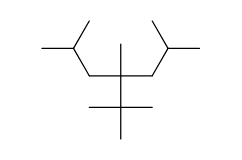
\includegraphics{smile-5613ea01d5a813b7cf528d9d04bd652915cea8b6}

4-tert-butyl-2,4,6-trimethylheptane

hay 2,4,6-trimethyl-4-(1,1-dimethylethyl)heptane

Tương tự như trên, ở vị trí carbon số 4 có nhánh phức tạp, trong đó carbon của nhánh phức tạp gắn vào mạch chính được đánh số 1 (xem hình). Tên nhánh phức tạp được cho vào ngoặc. Do đó tên alkane đã cho là 2,4,6-trimethyl-4-(1,1-dimethylethyl)heptane.\\
12.20*. a) Chỉ số octane càng cao, độ chịu nén trước khi phát nổ của xăng càng lớn nên chất lượng xăng càng tốt. Ví dụ xăng có chỉ số octane 92 dễ bị cháy khi nén hơn so với xăng có chỉ số octane 95 nên xăng có chỉ số octane 95 giá trị hơn xăng có chỉ số octane 92 . Tuy nhiên phải tuỳ vào tỉ số nén của động cơ để chọn xăng phù hợp. Động cơ có tỉ số nén thấp thì không cần dùng xăng có chỉ số octane cao.\\
b) Vì mẫu xăng trên chứa $80 \%$ thể tích là 2,2,4-trimethylpentane nên chỉ số octane của mẫu xăng là 80 .\\
12.21*. Ethanol có chỉ số octane cao hơn nhiều (khoảng 109) so với xăng. Các nhà máy lọc dầu thường pha ethanol với xăng để giúp tăng chỉ số octane. Hầu hết xăng ở Mỹ chứa ít nhất 10\% ethanol.\\
12.22*. RON là viết tắt của Research Octane Number, tức chỉ số octane nghiên cứu. Như vậy xăng RON 92 và xăng RON 95 có chỉ số octane lần lượt là 92 và 95 . Do đó xăng RON 95 có chỉ số octane cao hơn xăng RON 92.\\
12.23*. Ethanol có chỉ số octane cao hơn khá nhiều so với xăng thông thường, đạt ngưỡng khoảng 109. Do xăng E5 chứa 5\% ethanol và 95\% xăng RON 92 (theo thể tích) nên sẽ có chỉ số octane khoảng 92,85 .\\
Cách tính chỉ số octane của xăng E5:\\
Trong 100 L xăng E5 có 95 L xăng RON 92 và 5 L ethanol.\\
Có thể xem trong 95 L xăng RON 92 có $\frac{92 \times 95}{100}=87,4(\mathrm{~L})$ xăng có chỉ số octane là 100 , còn lại là $95-87,4=7,6(\mathrm{~L})$ xăng có chỉ số octane là 0 .

Vậy chỉ số octane của xăng E5 là $\frac{87,4 \times 100+5 \times 109+7,6 \times 0}{100}=92,85$.\\
Tương tự trong 100 L xăng E10 có 10 L ethanol và 90 L xăng RON 92. Có thể xem trong 90 L xăng A92 có $\frac{92 \times 90}{100}=82,8(\mathrm{~L})$ xăng có chỉ số octane là 100 , còn lại là $90-82,8=7,2(\mathrm{~L})$ xăng có chỉ số octane là 0 .

Do đó chỉ số octane của xăng E10 là $\frac{82,8 \times 100+10 \times 109+7,2 \times 0}{100}=93,70$. Như vậy hàm lượng ethanol càng cao thì chỉ số octane của xăng sinh học càng lớn.\\
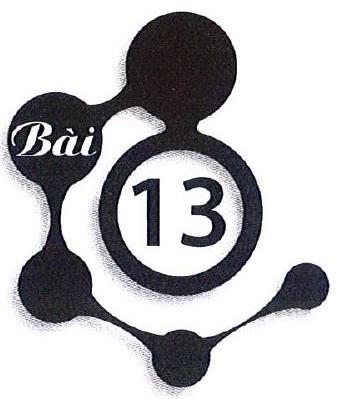
\includegraphics[max width=\textwidth, center]{2025_10_23_adad5b98d65ac6665838g-21}

\section*{HYDROCARBON KHÔNG NO}
13.1. Đáp án D. Lưu ý cis-but-2-ene cũng ở thể khí trong điều kiện thường do có nhiệt độ sôi là $4^{\circ} \mathrm{C}$.\\
13.2. Đáp án A . Có 3 alkyne $\mathrm{C}_{5} \mathrm{H}_{8}$ là đồng phân cấu tạo của nhau, gồm\\
$\mathrm{CH} \equiv \mathrm{C}-\mathrm{CH}_{2}-\mathrm{CH}_{2}-\mathrm{CH}_{3}$;\\
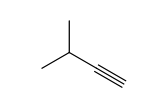
\includegraphics{smile-a128aae77d28996e052ddc768d40a3a5ad377355}\\
$\mathrm{CH}_{3}-\mathrm{C} \equiv \mathrm{C}-\mathrm{CH}_{2}-\mathrm{CH}_{3}$\\
13.3. Đáp án B. Có 2 alkene đã nêu có đồng phân hình học là $\mathrm{CH}_{3}-\mathrm{CH}_{2}-\mathrm{CH}=\mathrm{CH}-\mathrm{CH}_{3}$\\
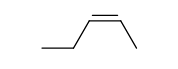
\includegraphics{smile-f750d262f4ed819a34c02ef3df1bd0fb83e95608}

cis-pent-2-ene\\
và $\mathrm{CH}_{3}-\mathrm{CH}_{2}-\mathrm{CH}=\mathrm{CH}-\mathrm{CH}_{2}-\mathrm{CH}_{3}$ :\\
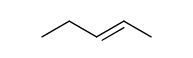
\includegraphics{smile-a89db969b4a6ed30442b55c9f18991fe22f3d838}

trans-pent-2-ene\\
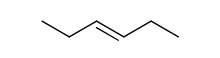
\includegraphics{smile-6db97c8948ae4a5b664f28cb83fd4d69f000ff80}

cis-hex-3-ene\\
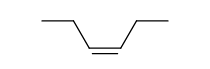
\includegraphics{smile-8a3ca3e8e3ed676b1bae93aaee74dd00c0f64d1c}

trans-hex-3-ene\\
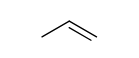
\includegraphics{smile-70953a262a35a9741377e9e9921c122d6aeca391}

propene\\
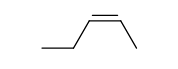
\includegraphics{smile-6a1224db25158221053806ff68599a1908795a66}

cis-pent-2-ene\\
13.4. Công thức khung phân tử các chất đã cho:\\
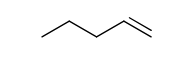
\includegraphics{smile-5db86fc38e43057ca5d40d72f4078da99083ec65}

pent-1-ene\\
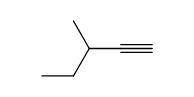
\includegraphics{smile-870a1adb5883b036bfd092ec760a4ed6c5059aba}

3-methylpent-1-yne\\
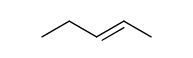
\includegraphics{smile-80914e69c179856ea2a218165ccf7f4b052a9bdf}

trans-pent-2-ene\\
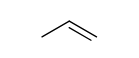
\includegraphics{smile-8ad0b51618f6c71690567b181b49a7daea4a4104}

( $\mathrm{t}_{\mathrm{s}}^{\circ}=-47,6^{\circ} \mathrm{C}$ )\\
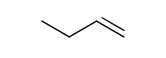
\includegraphics{smile-16234868fab4ee835b5757407315977999b89077}

( $\mathrm{t}_{\mathrm{s}}^{\circ}=-6,3^{\circ} \mathrm{C}$ )\\
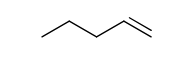
\includegraphics{smile-c3115ddee60253494ddd35759bfd70d44884c617}

( $\mathrm{t}_{\mathrm{s}}^{\circ}=30,1^{\circ} \mathrm{C}$ )\\
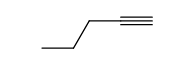
\includegraphics{smile-aa2fb3686c6ca48d6ae80cd0f28cc64cce4b3c1d}\\
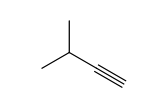
\includegraphics{smile-6b3c2e17e230e6042c143ff5fc405196386f85b2}

$\mathrm{CH}_{3}-\mathrm{C} \equiv \mathrm{C}-\mathrm{CH}_{2}-\mathrm{CH}_{3}$\\
pent-1-yne\\
3-methylbut-1-yne\\
pent-2-yne\\
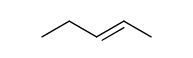
\includegraphics{smile-563646fc6a81bb37c8014c19555cfdd090946ac3}

cis-pent-2-ene\\
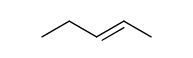
\includegraphics{smile-ac1916a6bb0e8767647d2c4030993449b466cc9a}

trans-pent-2-ene\\
13.5. a) (A): propene, (B): but-1-ene và (C): pent-1-ene.\\
b) Đi từ propene đến pent-1-ene, kích thước phân tử alkene tăng dần làm cho diện tích bề mặt tiếp xúc giữa chúng cũng tăng, tương tác van der Waals giữa các phân tử do đó cũng tăng dần, dẫn đến nhiệt độ sôi các alkene tăng dần. Ngoài ra, ở điều kiện thường, propene và but-1-ene là các chât khí trong khi pent-1-ene là chất lỏng vì tương tác van der Waals giữa các phân tử propene và but-1-ene chưa đủ lớn. Các phân tử alkene có từ 18 nguyên tử carbon trở lên ở thể rắn, do tương tác van der Waals giữa chúng là mạnh đáng kể.\\
13.6. Công thức cấu tạo của các alkene $\mathrm{C}_{5} \mathrm{H}_{10}$ :\\
$\mathrm{CH}_{3}-\mathrm{CH}_{2}-\mathrm{CH}_{2}-\mathrm{CH}=\mathrm{CH}_{2}$\\
$\mathrm{CH}_{3}-\mathrm{CH}_{2}-\mathrm{CH}=\mathrm{CH}-\mathrm{CH}_{3} \quad$ pent-2-ene\\
$\mathrm{CH}_{2}=\mathrm{CH}-\mathrm{CH}-\mathrm{CH}_{3}$ 3-methylbut-1-ene\\
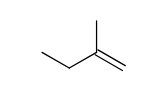
\includegraphics{smile-e7ce1eecf7434732b6a4644e5d7a7fd45bed61c6}

2-methylbut-1-ene\\
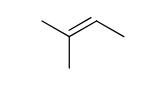
\includegraphics{smile-a08d301a8a3d50531fa9d33146828dcd476cb515}

2-methylbut-2-ene

Công thức cấu tạo của các alkyne $\mathrm{C}_{5} \mathrm{H}_{8}$ :

Chỉ pent-2-ene có đồng phân hình học là:\\
13.7. Đồng phân trans có tổng moment lưỡng cực thường triệt tiêu hoặc gần triệt tiêu, còn đồng phân cis có tổng moment lưỡng cực không triệt tiêu,\\
do đó đồng phân trans có nhiệt độ sôi thấp hơn đồng phân cis.\\
Ví dụ phân tử cis-but-2-ene và trans-but-2-ene đều chứa nhóm $-\mathrm{CH}_{3}$ là nhóm đẩy electron làm phân tử mỗi chất hình thành các moment lưỡng cực yếu C-C như trong hình bên dưới. Tuy nhiên, cis-but-2-ene có tổng moment lưỡng cực không triệt tiêu, còn trans-but-2-ene có tổng moment lưỡng cực triệt tiêu. Do đó cis-but-2-ene là phân tử phân cực nhẹ, trans-but-2-ene là phân tử không phân cực, dẫn đến nhiệt độ sôi của\\
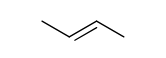
\includegraphics{smile-06ba4484842af8f9c690159ba5958ea9fa21c672}

cis-pent-2-ene (sôi ở $4^{\circ} \mathrm{C}$ )\\
cis-but-2-ene cao hơn so với trans-but-2-ene.

\includegraphics{smile-61351a8c6a4d79d57e5bd55e93902354882981a7}

trans-pent-2-ene (sôi ở $1^{\circ} \mathrm{C}$ )\\
13.8*. Tuy liên kết ba $\mathrm{C} \equiv \mathrm{C}$ của một alkyne giàu mật độ electron hơn so với liên kết đôi $\mathrm{C}=\mathrm{C}$ của một alkene tương ứng nhưng khả năng phản ứng cộng ( $\mathrm{X}_{2}, \mathrm{HX}, \mathrm{H}_{2} \mathrm{O}$ ) vào alkyne lại kém hơn vào alkene tương ứng. Điều này có thể giải thích là do nguyên tử carbon trong liên kết $\mathrm{C} \equiv \mathrm{C}$ ở trạng thái lai hoá sp , có độ âm điện lớn hơn các nguyên tử carbon trong liên kết $\mathrm{C}=\mathrm{C}$ ở trạng thái lai hoá $\mathrm{sp}^{2}$, làm cho các electron $\pi$ trong $\mathrm{C} \equiv \mathrm{C}$ bị giữ chặt hơn so với các electron $\pi$ trong $\mathrm{C}=\mathrm{C}$, dẫn đến khả năng phản ứng cộng ( $\mathrm{X}_{2}, \mathrm{HX}, \mathrm{H}_{2} \mathrm{O}$ ) của alkyne kém hơn alkene tương ứng.\\
Ví dụ ethylene nhanh chóng làm mất màu nước bromine, acetylene làm mất màu nước bromine chậm hơn. Tốc độ mất màu nước bromine của ethylene gấp 5 lần so với acetylene.\\
13.9*. Do nguyên tử bromine có độ âm điện lớn hơn nguyên tử carbon nên liên kết $\mathrm{C}-\mathrm{Br}$ bị phân cực mạnh về phía bromine, kết quả liên kết đôi của trans-2,3-dibromobut-2-ene có mật độ electron thấp hơn đáng kể so với liên kết đôi của trans-but-2-ene. Chính vì vậy khả năng phản ứng cộng bromine của trans-2,3-dibromobut-2-ene kém hơn so với trans-but-2-ene.\\
13.10*. Phản ứng cộng bromine vào liên kết ba $\mathrm{C} \equiv \mathrm{C}$ của một alkyne dễ hơn vào liên kết đôi $\mathrm{C}=\mathrm{C}$ của một dibromoalkene tương ứng. Điều này được giải thích là do nguyên tử bromine có độ âm diện mạnh, đã làm liên kết $\mathrm{C}-\mathrm{Br}$ phân cực mạnh về phía bromine, làm mật độ electron trên liên kết đôi của dibromoalkene kém hơn hẳn so với trên liên kết ba của alkyne tương ứng.\\
13.11. Phương trình hoá học của các phản ứng:\\
a) $\mathrm{CH}_{3}-\mathrm{CH}_{2}-\mathrm{CH}=\mathrm{CH}_{2}+\mathrm{Br}_{2} \longrightarrow \mathrm{CH}_{3}-\mathrm{CH}_{2}-\mathrm{CH}-\stackrel{\mathrm{Br}}{\mathrm{C}} \mathrm{H}_{2}$\\
b) $\mathrm{CH} \equiv \mathrm{C}-\mathrm{CH}_{3}+2 \mathrm{Br}_{2} \xrightarrow{1: 2} \underbrace{\mathrm{Br}}_{\substack{\mathrm{C} \\ \mathrm{C}}}-\stackrel{\mathrm{Br}}{\underset{\mathrm{Br}}{\mathrm{I}}}-\mathrm{CH}_{3}$\\
$B r \quad B r$\\
\includegraphics[max width=\textwidth, center]{2025_10_23_adad5b98d65ac6665838g-22(3)}\\
\includegraphics[max width=\textwidth, center]{2025_10_23_adad5b98d65ac6665838g-22(2)}\\
\includegraphics[max width=\textwidth, center]{2025_10_23_adad5b98d65ac6665838g-22(4)}\\
\includegraphics[max width=\textwidth, center]{2025_10_23_adad5b98d65ac6665838g-22(1)}\\
13.12. Phương trình hoá học phản ứng:\\
\includegraphics[max width=\textwidth, center]{2025_10_23_adad5b98d65ac6665838g-22}\\
13.13.\\
a) $\mathrm{CH}_{2}=\mathrm{CH}_{2}+\mathrm{H}_{2} \mathrm{O} \xrightarrow{\mathrm{H}^{+}, 160^{\circ} \mathrm{C}} \mathrm{C}_{2} \mathrm{H}_{5} \mathrm{OH}$\\
b) $\mathrm{CH}_{3}-\mathrm{CH}_{2}-\mathrm{CH}=\mathrm{CH}_{2}+\mathrm{H}_{2} \mathrm{O} \xrightarrow{\mathrm{H}^{+}, 90^{\circ} \mathrm{C}} \mathrm{CH}_{3}-\mathrm{CH}_{2}-\underset{\mathrm{OH}}{\mathrm{CH}}-\mathrm{CH}_{3}$\\
c) $\mathrm{CH}_{3}-\mathrm{CH}=\underset{\mathrm{C} \mathrm{H}_{3}}{\mathrm{C}}-\mathrm{CH}_{3}+ \mathrm{H}_{2} \mathrm{O}$

$$
\mathrm{H}^{+}, 20^{\circ} \mathrm{C}
$$

\includegraphics{smile-9636f45d2488f28c5a61ad001e66297d25ba75b0}\\
13.14. Thuốc thử để phân biệt 2 chất lỏng mất nhãn gồm hexane và hex-1-ene là nước bromine. Tuy nhiên cũng có thể dựa vào phổ hồng ngoại của chúng để phân biệt như sau:\\
\includegraphics[max width=\textwidth, center]{2025_10_23_adad5b98d65ac6665838g-23(2)}\\
\includegraphics[max width=\textwidth, center]{2025_10_23_adad5b98d65ac6665838g-23(3)}

Trong phổ IR của hex-1-ene có peak khoảng $1650 \mathrm{~cm}^{-1}$ vì đặc trưng cho liên kết đôi $C=C$ nên có thể dễ dàng nhận ra hex-1-ene. Ngoài ra, hex-1-ene có nhóm vinyl ( $\mathrm{CH}_{2}=\mathrm{CH}-$ ) nên cũng phải có peak đặc trưng khoảng $3080 \mathrm{~cm}^{-1}$. Trong khi đó, phổ IR của hexane không có các peak này nên có thể dễ dàng phân biệt chúng.\\
13.15. a) Có thể dùng dung dịch $\mathrm{AgNO}_{3}$ trong $\mathrm{NH}_{3}$ để phân biệt chúng theo phương pháp hoá học.\\
b) Phương pháp vật lí là dùng phổ hồng ngoại để phân biệt. Đặc trưng phổ hồng ngoại của các alk-1-yne là có peak khoảng $3300 \mathrm{~cm}^{-1}$, trong khi các alkyne khác không có peak này. Do đó phổ hồng ngoại có peak đặc trưng khoảng $3300 \mathrm{~cm}^{-1}$ là hex-1-yne. Chất còn lại là hex-2-yne.\\
\includegraphics[max width=\textwidth, center]{2025_10_23_adad5b98d65ac6665838g-23(1)}\\
\includegraphics[max width=\textwidth, center]{2025_10_23_adad5b98d65ac6665838g-23}\\
13.16*. a) Nguyên tử carbon ở trạng thái lai hoá $s p$ có tỉ lệ đóng góp của orbital $s$ là $50 \%$, cao hơn so với nguyên tử carbon ở trạng thái lai hoá $s p^{2}(33,3 \%)$ và nguyên tử carbon ở trạng thái lai hoá $s p^{3}(25 \%)$ nên orbital lai hoá $s p$ của nguyên tử carbon ở gần hạt nhân hơn, dẫn đến nguyên tử carbon lai hoá sp có độ âm điện cao hơn. Vì thế nguyên tử hydrogen liên kết trực tiếp với các nguyên tử carbon mang liên kết ba có tính linh động.\\
b) Hydrocarbon có 3 nguyên tử hydrogen linh động có thể là:\\
\includegraphics{smile-4a5dfae778cec4836c446f56cb00f910e1da4e22}\\
13.17. Phương trình phản ứng xảy ra:

$$
3 \mathrm{CH} \equiv \mathrm{CH} \xrightarrow{\mathrm{Fe}, 600^{\circ} \mathrm{C}} \mathrm{C}_{6} \mathrm{H}_{6}
$$

Với 150 gam acetylene, trên lí thuyết phải thu được 150 gam benzene, nhưng thực tế chỉ thu được 90 gam benzene nên hiệu suất phản ứng đạt:

$$
\frac{90 \times 100}{150}=60 \%
$$

13.18. Đó là do chuối khi chuẩn bị chín sẽ giải phóng một loại hormone thực vật ở thể khí là ethylene, giúp đẩy nhanh quá trình chín không những của chuối, mà còn nhiều loại quả khác nhau. Nhờ đó quả bơ cũng được đẩy nhanh chín theo.\\
13.19. Các phương trình phản ứng xảy ra:

$$
\begin{gathered}
\mathrm{CH}_{2}=\mathrm{CH}_{2}+\mathrm{Cl}_{2} \longrightarrow \mathrm{CH}_{2} \mathrm{Cl}-\mathrm{CH}_{2} \mathrm{Cl} \\
\mathrm{CH}_{2} \mathrm{Cl}-\mathrm{CH}_{2} \mathrm{Cl}+\mathrm{KOH} \xrightarrow[\text { ethanol }]{\mathrm{CCl}_{4}, 60^{\circ} \mathrm{C}} \mathrm{CH}_{2}=\mathrm{CH}-\mathrm{Cl}+\mathrm{KCl}+\mathrm{H}_{2} \mathrm{O}
\end{gathered}
$$

13.20. Phương trình phản ứng xảy ra:

$$
2 \mathrm{CH}_{3} \mathrm{COOH}+\mathrm{CH}_{2}=\mathrm{CH}_{2}+2 \mathrm{O}_{2} \xrightarrow[5-9 \text { bar }]{\mathrm{Pd}, 175-200^{\circ} \mathrm{C}} \mathrm{CH}_{3} \mathrm{COOCH}=\mathrm{CH}_{2}+\mathrm{H}_{2} \mathrm{O}
$$

13.21. a) $\mathrm{CH}_{2}=\mathrm{CH}_{2}+\mathrm{Cl}_{2} \longrightarrow \mathrm{CH}_{2} \mathrm{Cl}-\mathrm{CH}_{2} \mathrm{Cl}$\\
$\mathrm{CH}_{2} \mathrm{Cl}-\mathrm{CH}_{2} \mathrm{Cl}+\mathrm{KOH} \xrightarrow[\text { ethanol }]{\mathrm{CCl}_{4}, 60^{\circ} \mathrm{C}} \mathrm{CH}_{2}=\mathrm{CH}-\mathrm{Cl}+\mathrm{KCl}+\mathrm{H}_{2} \mathrm{O}$\\
$4 \mathrm{HCl}+\mathrm{O}_{2} \xrightarrow{\mathrm{t}^{\circ}} 2 \mathrm{Cl}_{2}+2 \mathrm{H}_{2} \mathrm{O}$\\
b) $\mathrm{CH}_{2}=\mathrm{CH}_{2}+\mathrm{Cl}_{2} \longrightarrow \mathrm{CH}_{2} \mathrm{Cl}-\mathrm{CH}_{2} \mathrm{Cl}$\\
$\mathrm{CH}_{2} \mathrm{Cl}-\mathrm{CH}_{2} \mathrm{Cl} \xrightarrow{500^{\circ} \mathrm{C}} \mathrm{CH}_{2}=\mathrm{CH}-\mathrm{Cl}+\mathrm{HCl}$\\
$\mathrm{CH} \equiv \mathrm{CH}+\mathrm{HCl} \xrightarrow{\mathrm{Hg}^{2+}} \mathrm{CH}_{2}=\mathrm{CHCl}$\\
Sơ đồ b) tích hợp các phương pháp sản xuất vinyl chloride, còn sơ đồ a) thải sản phẩm phụ là $\mathrm{H}_{2} \mathrm{O}$ ra môi trường.\\
14.8. Đáp án $B$.

Đánh số trên vòng benzene sao cho tổng chỉ số các nhánh là nhỏ nhất, do đó không thể đánh số 1 cho nhánh bromo, vì tổng chỉ số các nhánh khi đó là $(1+3+4)=8$ lớn hơn cách đánh số đúng như dưới đây có tổng chỉ số các nhánh là $(1+2+4)=7$.\\
\includegraphics{smile-63794991722ed695334717d0eb213da7daf9d4c4}

4-bromo-1-chloro-2-nitrobenzene\\
14.9. Đáp án B.

Đánh số trên vòng benzene sao cho tổng chỉ số các nhánh là nhỏ nhất. Do đó hợp chất đã cho có tên gọi như sau:\\
\includegraphics{smile-afb0b727b173af823c8d7ca21cbe27b2d272f802}

4-bromo-2-methyl-1-nitrobenzene\\
14.10*. a) Trên đồ thị, ta thấy ở cùng nhiệt độ như nhau, áp suất hơi của acetone lớn nhất, tiếp đến là tetrahydrofuran và cuối cùng là benzene. Do đó ở cùng nhiệt độ như nhau, acetone là chất dễ bay hơi nhất.\\
b) Căn cứ vào đồ thị đã cho, ở điều kiện áp suất 1 atm hay 760 torr, các chất acetone, tetrahydrofuran và benzene lần lượt có nhiệt độ sôi tương ứng là $56^{\circ} \mathrm{C}, 65^{\circ} \mathrm{C}$ và $80,1^{\circ} \mathrm{C}$.\\
\includegraphics[max width=\textwidth, center]{2025_10_23_adad5b98d65ac6665838g-25}\\
c) Nếu đặt một cốc chứa benzene lỏng vào trong một bình kín chứa hơi benzene ở $73^{\circ} \mathrm{C}$ và 600 torr. Sau 10 phút, thể tích chất lỏng trong cốc vẫn không thay đổi. Đó là do trong điều kiện nhiệt độ và áp suất đã nêu, áp suất hơi của benzene trong cốc và áp suất hơi trong bình kín bằng nhau nên không xảy ra sự chuyển pha của benzene.\\
14.11. Có 8 arene sau:\\
\includegraphics{smile-ba8af16fe8ebec3397da9552da37adc3e0ae54c8}

propylbenzene\\
\includegraphics{smile-6144f280c1b20172d0894b2293004c25ccf30891}

isopropylbenzene\\
(cumene)\\
\includegraphics{smile-e096ea111161a8893d9c9855a994851895f5bbcf}

1-ethyl-2-methylbenzene\\
\includegraphics{smile-c5f2d81920610ebe8f4097c1fef363271a58a233}

1-ethyl-3-methylbenzene\\
\includegraphics{smile-6f9512096ca8d843dad2548505da770fb34c92dd}

1-ethyl-4-methylbenzene\\
\includegraphics{smile-fad46b4c4a705bdf1a061a23bc4c82050d65ebd2}

1,2,3-trimethylbenzene\\
\includegraphics{smile-00e215c6c0e2d7504886fa7526f60de3fe529471}

1,2,4-trimethylbenzene\\
\includegraphics{smile-f791be6e9fcbed6a6f811ba95952381f360b150f}

1,3,5-trimethylbenzene\\
14.12. Trời lạnh làm cho quá trình cháy xảy ra khó hoàn toàn so với trời nắng, nóng. Do đó carbon monoxide đạt mức cao nhất khi thời tiết lạnh.\\
14.13. Phần trăm tối đa cumene giảm thiểu khi có bộ chuyển đổi xúc tác so với trường hợp không có bộ chuyển đổi xúc tác là $\frac{0,002-0,0009}{0,002} \times 100=55 \%$.\\
14.14. a) Bình quân một tháng, mỗi chiếc chạy 3000 km , do đó trong một năm, mỗi chiếc chạy quãng đường là 36000 km , phát thải tối đa

$$
0,0009 \times 36000=32,4(\mathrm{~g}) \text { cumene. }
$$

Vậy 1000000 xe ô tô trong một năm phát thải tối đa

$$
1000000 \times 32,4=32400000(\mathrm{~g})=32,4 \text { (tấn) cumene. }
$$

b) Trong một tháng, một cửa hàng với quy mô 10 máy photocopy sử dụng bình quân liên tục:

$$
10 \times 12 \times 30=3600 \text { (giờ). }
$$

Như vậy, trong một tháng, một cửa hàng với quy mô như trên phát thải tối đa:

$$
220 \times 3600=792000(\mu \mathrm{~g})=0,792(\mathrm{~g})
$$

Vậy 1000 cửa hàng trong một tháng phát thải tối đa là\\
$1000 \times 0,792=792(\mathrm{~g})$ cumene.

\subsection*{14.15.}
a)\\
\includegraphics[max width=\textwidth, center]{2025_10_23_adad5b98d65ac6665838g-26}\\
b)\\
\includegraphics[max width=\textwidth, center]{2025_10_23_adad5b98d65ac6665838g-26(2)}\\
c)\\
\includegraphics[max width=\textwidth, center]{2025_10_23_adad5b98d65ac6665838g-26(4)}\\
d)\\
\includegraphics[max width=\textwidth, center]{2025_10_23_adad5b98d65ac6665838g-26(6)}\\
e)\\
\includegraphics[max width=\textwidth, center]{2025_10_23_adad5b98d65ac6665838g-26(8)}\\
g) $\mathrm{C}_{6} \mathrm{H}_{5} \mathrm{C}\left(\mathrm{CH}_{3}\right)_{3}+\mathrm{KMnO}_{4}+\mathrm{H}_{2} \mathrm{SO}_{4} \xrightarrow{8 \mathrm{Q}^{\circ} \mathrm{C}}$ Không xảy ra\\
14.16. Phương trình biểu diễn các sản phẩm monobromo thu được trong quá trình bromine hoá $p$-xylene, o-xylene và $m$-xylene:\\
\includegraphics[max width=\textwidth, center]{2025_10_23_adad5b98d65ac6665838g-26(1)}\\
\includegraphics[max width=\textwidth, center]{2025_10_23_adad5b98d65ac6665838g-26(5)}\\
14.17. Với công thức phân tử $\mathrm{C}_{9} \mathrm{H}_{12},(\mathrm{H})$ không làm mất màu nước bromine nhưng $(\mathrm{H})$ làm mât màu dung dịch $\mathrm{KMnO}_{4}$ đã được acid hoá và tạo terephthalic acid nên $(\mathrm{H})$ là một arene có công thức cấu tạo:\\
\includegraphics[max width=\textwidth, center]{2025_10_23_adad5b98d65ac6665838g-26(3)}

Phương trình phản ứng:\\
\includegraphics[max width=\textwidth, center]{2025_10_23_adad5b98d65ac6665838g-26(7)}\\
14.18. a) Quan sát dữ kiện đề cho, ta thấy các nhóm thế alkyl làm tăng hoạt vòng benzene, các nhóm thế halogen và ester làm giảm hoạt vòng benzene.\\
b) Toluene có 2 vị trí ortho, 2 vị trí meta và 1 vị trí para nên:

\begin{itemize}
  \item Phần trăm sản phẩm thế ortho là $\frac{2 \times 43 \times 100}{43+43+3+3+55}=58,5 \%$.
  \item Phần trăm sản phẩm thế meta là $\frac{2 \times 3 \times 100}{43+43+3+3+55}=4,08 \%$.
  \item Phần trăm sản phẩm thế para là $\frac{55 \times 100}{43+43+3+3+55}=37,41 \%$.\\
c) tert-butylbenzene cũng có 2 vị trí ortho, 2 vị trí meta và 1 vị trí para nên:
  \item Phần trăm sản phẩm thế ortho là $\frac{2 \times 8 \times 100}{8+8+4+4+75}=16,16 \%$.
  \item Phần trăm sản phẩm thế meta là $\frac{2 \times 4 \times 100}{8+8+4+4+75}=8,08 \%$.
  \item Phần trăm sản phẩm thế para là $\frac{75 \times 100}{8+8+4+4+75}=75,76 \%$.\\
d) Nhóm tert-butyl có kích thước lớn làm cản trở sự tấn công tại các vị trí ortho nên phần trăm sản phẩm thế ortho vào tert-butylbenzene giảm so với toluene.\\
e) Tỉ lệ phần trăm sản phẩm thế meta trong các phản ứng nitro hoá toluene và tert-butylbenzene đều thấp, chứng tỏ các nhóm alkyl làm cho phản ứng có hướng thế ưu tiên vào các vị trí ortho và para hơn so với vào vị trí meta.\\
14.19.\\
a) Chlorobenzene có 2 vị trí ortho, 2 vị trí meta và 1 vị trí para nên:
  \item Phần trăm sản phẩm thế ortho là $\frac{2 \times 0,03 \times 100}{0,03+0,03+0,14}=30 \%$.
  \item Phần trăm sản phẩm thế meta là $0 \%$.
  \item Phần trăm sản phẩm thế para là $\frac{0,14 \times 100}{0,03+0,03+0,14}=70 \%$.
\end{itemize}

Methyl benzoate cũng có 2 vị trí ortho, 2 vị trí meta và 1 vị trí para nên:

\begin{itemize}
  \item Phần trăm sản phẩm thế ortho là
\end{itemize}

$$
\frac{2 \times 0,0025 \times 100}{0,0025+0,0025+0,008+0,008+0,001}=22,73 \%
$$

\begin{itemize}
  \item Phần trăm sản phẩm thế meta là
\end{itemize}

$$
\frac{2 \times 0,008 \times 100}{0,0025+0,0025+0,008+0,008+0,001}=72,73 \%
$$

\begin{itemize}
  \item Phần trăm sản phẩm thế para là
\end{itemize}

$$
\frac{0,001 \times 100}{0,0025+0,0025+0,008+0,008+0,001}=4,55 \%
$$

b) Khả năng nitro hoá của chlorobenzene và methyl benzoate giảm hơn so với khả năng nitro hoá của toluene và tert-butylbenzene. Tuy nhiên hướng thế của chlorobenzene ưu tiên vào các vị trí ortho và para, trong khi hướng thế của methyl benzoate ưu tiên vào vị trí meta.\\
c) Quy luật thế vào vòng benzene: Khi trong vòng benzene đã có sẵn một nhóm alkyl, như - $\mathrm{CH}_{3}$ (hay các nhóm - $\mathrm{OH},-\mathrm{NH}_{2}, \ldots$ ), phản ứng thế vào vòng sẽ dễ dàng hơn, với hướng thế ưu tiên vào các vị trí ortho và para. Ngược lại, nếu vòng benzene đã có sẵn một nhóm $-\mathrm{NO}_{2}$ (hay -COOH , $-\mathrm{COOR},-\mathrm{CHO}, \ldots$ ), phản ứng thế vào vòng sẽ khó hơn và hướng thế ưu tiên vào các vị trí meta. Nhóm -Cl làm khả năng phản ứng thế trong vòng benzene khó hơn, nhưng hướng thế lại ưu tiên thế vào các vị trí ortho và para.\\
14.20. Để giảm thiểu sự tiếp xúc với benzene, cần chú ý:

\begin{itemize}
  \item Khi pha chế xăng, cần phải sử dụng mặt nạ chống độc để tránh hít phải hơi xăng.
  \item Khi đổ xăng cần phải được tiến hành trong điều kiện thông thoáng.
  \item Cần phải bảo quản xăng trong các thùng kín.
  \item Không pha chế hoặc xử lí xăng trong nhà hoặc ga ra.
  \item Thùng chứa và máy móc vận hành xăng không để trong nhà.
  \item Cẩn thận trong khi làm việc với các loại keo dán, chất kết dính, sản phẩm tẩy rửa, dụng cụ tẩy sơn,...\\
Ngoài ra hơi benzene cũng có trong khói thuốc lá, khí thải của nhiều ngành công nghiệp và ô tô. Những người sống gần đường cao tốc hoặc các khu công nghiệp có thể dễ tiếp xúc với benzene hơn.\\
14.21. Phương trình phản ứng dealkyl hoá toluene thành benzene.\\
\includegraphics[max width=\textwidth, center]{2025_10_23_adad5b98d65ac6665838g-27}\\
14.22*. Biến thiên enthalpy của quá trình hydrogen hoá cyclohexene và cyclohexa-1,3-diene thành cyclohexane lần lượt là $-120 \mathrm{~kJ} / \mathrm{mol}$ và $-240 \mathrm{~kJ} / \mathrm{mol}$, do đó biến thiên enthalpy của quá trình hydrogen hoá benzene được mong đợi sẽ là $3 \times 120=-360(\mathrm{~kJ} / \mathrm{mol})$. Tuy nhiên thực\\
tế biến thiên enthalpy của quá trình hydrogen hoá benzene chỉ là $-208(\mathrm{~kJ} / \mathrm{mol})$ (xem sơ đồ minh hoạ), cho thấy phân tử benzene không thể chứa ba liên kết đôi. Nói khác đi, các liên kết $\pi$ được định vị trên toàn bộ vòng benzene, nên không thể gọi benzene là cyclohexa-1,3,5-trien.\\
\includegraphics[max width=\textwidth, center]{2025_10_23_adad5b98d65ac6665838g-28(3)}
\end{itemize}

Năm 1929, nhà nữ bác học người Anh, Kathleen Lonsdale (1903 - 1971), đã sử dụng phương pháp phân tích nhiễu xạ tia $X$ để chỉ ra rằng tất cả độ dài liên kết $\mathrm{C}-\mathrm{C}$ trong benzene là giống hệt nhau. Khoảng cách này nhỏ hơn độ dài của liên kết $\mathrm{C}-\mathrm{C}$ và dài hơn của liên kết $\mathrm{C}=\mathrm{C}$. Điều này cho thấy ba liên kết $\pi$ trong phân tử benzene phải được trải đều trên toàn bộ vòng benzene ${ }^{(*)}$, cũng có nghĩa benzene không có cấu trúc của cyclohexa-1,3,5-triene.\\
\includegraphics[max width=\textwidth, center]{2025_10_23_adad5b98d65ac6665838g-28}

\begin{itemize}
  \item Sự hình thành liên kết $\sigma$ và hệ liên hợp $\pi$ trong phân tử benzene\\
14.23*. Khi vòng benzene có gắn nhóm thế alkyl, phản ứng thế nguyên tử hydrogen ở vòng benzene xảy ra dễ dàng hơn so với benzene và ưu tiên thế vào vị trí ortho hoặc para so với nhóm alkyl. Do đó $m$-bromoethylbenzene chỉ tạo thành ở dạng vết (<1\%).\\
Tuy nguyên tử bromine đã ưu tiên thế vào các vị trí ortho và para, nhưng phản ứng thế ở vị trí ortho khó khăn hơn so với vị trí para, do bị cản trở không gian. Do đó o-bromoethylbenzene ( $38 \%$ ) hình thành it hơn so với $p$-bromoethylbenzene ( $62 \%$ ).
\end{itemize}

\footnotetext{${ }^{()}$Tạo hệ liên hợp $\pi$.
}\section*{ÔN TÂP CHƯONG 4}
OT4.1. Đáp án D. Phương trình phản ứng của 2,2,3,3-tetramethylbutane với chlorine:\\
\includegraphics[max width=\textwidth, center]{2025_10_23_adad5b98d65ac6665838g-28(1)}

OT4.2. Đáp án A . Các alkene có đồng phân hình học là $\mathrm{CH}_{3} \mathrm{CH}=\mathrm{CHCH}_{3}$ và $\mathrm{CH}_{3} \mathrm{CH}=\mathrm{CHC}_{2} \mathrm{H}_{5}$.

OT4.3. Đáp án C. Phương trình phản ứng xảy ra:\\
\includegraphics[max width=\textwidth, center]{2025_10_23_adad5b98d65ac6665838g-28(2)}

OT4.4. a) Butane có áp suất hoá hơi thấp nhất trong số 3 alkane đã nêu là $2,3 \mathrm{~atm}$, do đó butane dễ hoá lỏng nhất.\\
b) Methane có áp suất hoá hơi lớn nhất là 320 atm nên methane khó hoá lỏng nhất. Để giữ được áp suất cực lớn này, bình chứa methane phải là thép cực bền.\\
OT4.5. Số mol propane $=\frac{12000}{44} \mathrm{~mol}$.\\
Do đó thể tích khí propane $=\frac{12000 \times 24,79}{44}=6761(\mathrm{~L})$.\\
OT4.6. a) Biểu đồ cho thấy có 4 phân tử alkane ở thể khí trong điều kiện thường là $\mathrm{CH}_{4}, \mathrm{C}_{2} \mathrm{H}_{6}, \mathrm{C}_{3} \mathrm{H}_{8}$ và $\mathrm{C}_{4} \mathrm{H}_{10}$.\\
b) Neopentane có công thức câu tạo là\\
\includegraphics{smile-3bd9d41396a616d3659ed529031971e7de8b34ff}\\
nên có cấu trúc đối xứng cao, phân tử xem như có dạng hình cầu, do đó tương tác van der Waals giữa các phân tử neopentane rất yếu, dẫn đến nhiệt độ sôi của neopeatane là $9,5^{\circ} \mathrm{C}$.\\
Vì thế tuy có 5 nguyên tử carbon trong phân tử nhưng neopentane là một alkane ở thể khí trong điều kiện thường.\\
c) Propane có áp suất hoá hơi là 850 kPa , trong khi butane là 230 kPa nên dụng cụ chứa propane lỏng phải là thép.

\begin{center}
\begin{tabular}{|c|l|l|}
\hline
 & \multicolumn{1}{|c|}{Propane} & \multicolumn{1}{|c|}{Butane} \\
\hline
Bảo quản & Thép do phải chịu áp suất cao. & \begin{tabular}{l}
Không cần thiết là thép, do \\
không phải chịu áp suât cao \\
(như bật lửa gas). \\
\end{tabular} \\
\hline
Độ an toàn & \begin{tabular}{l}
Thấp do dễ bay hơi, vì thế nên \\
được sử dụng ngoài trời. \\
\end{tabular} & \begin{tabular}{l}
Cao do khó bay hơi hơn, vì thế \\
nên có thể sừ dụng trong phòng. \\
\end{tabular} \\
\hline
Đặc điểm & Sử dụng tốt ngay khi trời lạnh. & Không sử dụng tốt khi trời lạnh. \\
\hline
\end{tabular}
\end{center}

OT4.7. Nhiệt lượng cần cung cấp trên lí thuyết để đun nóng 1 L nước hay 1000 gam nước từ $25^{\circ} \mathrm{C}$ lên $100^{\circ} \mathrm{C}$ là:

$$
Q=1000 \times(100-25) \times 4,2=315000(\mathrm{~J})=315(\mathrm{~kJ}) .
$$

Khối lượng propane trên lí thuyết cần là:

$$
\mathrm{m}_{\mathrm{C}_{3} \mathrm{H}_{8} \mathrm{LT}}=\frac{44 \times 315}{2220}=6,24(\mathrm{~g}) .
$$

Khối lượng propane thực tế cần lấy:

$$
\mathrm{m}_{\mathrm{C}_{3} \mathrm{H}_{8} \mathrm{TT}}=\frac{6,24 \times 100}{75}=8,32(\mathrm{~g}) .
$$

OT4.8. Thể tích ethylene có trong phòng ủ thể tích $50 \mathrm{~m}^{3}$, tức 50000 L là:

$$
V=\frac{50000 \times 140}{1000000}=7(\mathrm{~L})
$$

Khối lượng ethylene cần thiết:

$$
m=\frac{7 \times 28}{24,79}=7,9(g) .
$$

OT4.9. Alkyne $\mathrm{C}_{4} \mathrm{H}_{6}$ có 2 đồng phân là but-1-yne và but-2-yne. Đặc trưng phổ hồng ngoại của các alk-1-yne là có peak khoảng $3300 \mathrm{~cm}^{-1}$ (xem hình dưới), do đó phổ hồng ngoại của alkyne (A) cho thấy (A) là but-2-yne và (B) là but-1-yne.\\
\includegraphics[max width=\textwidth, center]{2025_10_23_adad5b98d65ac6665838g-29(1)}\\
\includegraphics[max width=\textwidth, center]{2025_10_23_adad5b98d65ac6665838g-29}

OT4.10. Tên các hợp chất đã cho là:\\
\includegraphics{smile-09fe149c5c44110826675d0a11d7a8f063481cb8}

1,3-dichlorobenzene\\
(hay $m$-dichlorobenzene)\\
\includegraphics{smile-5320ab1bd2a8cd780de0628e72d63f8b48a85a39}

1-phenyl-4-methylhexane\\
\includegraphics[max width=\textwidth, center]{2025_10_23_adad5b98d65ac6665838g-30(5)}

Lưu ý: Hợp chât d) không gọi 1-methyl-2,4,6-trinitrotoluene do tổng các chỉ số lớn hơn so với cách gọi 2-methyl-1,3,5-trinitrobenzene.

OT4.11. a) Khi hydrocarbon vừa có liên kết đôi, vừa có liên kết ba, chú ý đánh số ưu tiên liên kết đôi hơn liên kết ba. Tên hydrocarbon đã cho là:

$$
\begin{aligned}
& \stackrel{5}{\mathrm{CH}} \equiv \stackrel{4}{\mathrm{C}}-\stackrel{3}{\mathrm{C}} \mathrm{H}_{2}-\stackrel{2}{\mathrm{C}} \mathrm{H}=\stackrel{1}{\mathrm{CH}_{2}} \\
& \text { pent-1-ene-4-yne }
\end{aligned}
$$

b) Dựa vào phương trình phản ứng:\\
\includegraphics[max width=\textwidth, center]{2025_10_23_adad5b98d65ac6665838g-30(2)}\\
thì tốc độ cộng bromine vào liên kết đôi lớn hơn rất nhiều so với vào liên kết ba. Điều này cũng phù hợp khi ethylene và acetylene đều có khả năng làm mất màu nước bromine ở ngay điều kiện thường, nhưng tốc độ mất màu của ethylene nhanh hơn so với acetylene. Như vậy alkene dễ cho phản ứng cộng ( $\mathrm{X}_{2}, \mathrm{HX}, \mathrm{H}_{2} \mathrm{O}$ ) hơn so với alkyne.

OT4.12. Với công thức $\mathrm{C}_{10} \mathrm{H}_{14},(\mathrm{H})$ không làm mất màu nước brom nhưng $(\mathrm{H})$ làm mất màu dung dịch $\mathrm{KMnO}_{4}$ đã được acid hoá, tạo terephthalic acid là sản phẩm hữu cơ duy nhất nên $(\mathrm{H})$ là một arene có công thức cấu tạo:\\
\includegraphics[max width=\textwidth, center]{2025_10_23_adad5b98d65ac6665838g-30}

\begin{figure}[h]
\begin{center}
\captionsetup{labelformat=empty}
\caption{Phương trình phản ứng của \$(\textbackslash mathrm\{H})\$ :\}\\
  \includegraphics[width=\textwidth]{2025_10_23_adad5b98d65ac6665838g-30(6)}
\end{center}
\end{figure}

$(\mathrm{K})$ có công thức $\mathrm{C}_{10} \mathrm{H}_{14}$, (K) không làm mất màu nước bromine nhưng (K) làm mất màu dung dịch $\mathrm{KMnO}_{4}$ đã được acid hoá, tạo 2 sản phẩm hữu cơ là terephthalic acid và chất $(X)$ nên $(K)$ là một arene có công thức cấu tạo:\\
\includegraphics[max width=\textwidth, center]{2025_10_23_adad5b98d65ac6665838g-30(1)}

Phương trình phản ứng của ( K ):\\
\includegraphics[max width=\textwidth, center]{2025_10_23_adad5b98d65ac6665838g-30(3)}\\
\includegraphics[max width=\textwidth, center]{2025_10_23_adad5b98d65ac6665838g-30(4)}

Do đó $(\mathrm{X})$ là $\mathrm{CH}_{3} \mathrm{COOH}$.\\
OT4.13*. Nhóm methoxy trong anisole làm tăng hoạt ${ }^{*}$ ) mạnh vòng benzene đến mức anisole nhanh chóng bromine hoá trong nước bromine mà không cần xúc tác, trong khi toluene cần có xúc tác là $\mathrm{FeBr}_{3}$ hoặc $\mathrm{AlBr}_{3}$.

OT4.14*. Trong $m$-xylene, vị trí ortho của cả 2 nhóm methyl hoặc vị trí ortho của nhóm methyl này nhưng là vị trí para của nhóm methyl kia đều thuận lợi cho hướng thế vào vòng benzene. Trong khi ở p-xylene, vị trí ortho của nhóm methyl này lại là vị trí meta của nhóm methyl kia. Điều này giúp $m$-xylene tham gia phản ứng nitro hoá nhanh hơn p-xylene 100 lần.

\footnotetext{(") Nhóm - $\mathrm{CH}_{3}$ và nhóm $\mathrm{CH}_{3} \mathrm{O}$ - đều có khả năng tăng hoạt vòng benzene, nhưng nhóm $\mathrm{CH}_{3} \mathrm{O}$ tăng hoạt vòng benzene mạnh hơn nhiều so với nhóm $-\mathrm{CH}_{3}$.
}Vị trí ortho của cả hai nhóm methyl\\
\includegraphics[max width=\textwidth, center]{2025_10_23_adad5b98d65ac6665838g-31(2)}

\section*{Chưong 5. DẪN XUAǴT HALOGEN ALCOHOL - PHIBNOL}
Baii

\section*{15 DẪN XUẤT HALOGEN}
15.1. Đáp án $C$.\\
15.2. Đáp án $A$.\\
15.3. Đáp án B.\\
15.4. Đáp án $D$.\\
15.5. Đáp án B.\\
\includegraphics{smile-5e50fcb79f22bf640e2aa800ba8b14799650d8d6}

1,1,1,2-tetrafluoroethane\\
15.6. Đáp án $B$.\\
15.7. Đáp án $C$.\\
15.8. Đáp án $B$.\\
15.9. Đáp án B.\\
\includegraphics{smile-f87707cdd5c233c19d8d82b02c096ebe178e9822}

1,1,1,3,3-pentafluorobutane\\
15.10. Đáp án D.\\
15.11. a) Tên gọi của các hợp chất:\\
b) Công thức cấu tạo của 4-chloro-3,4-dimethylpent-2-ene:\\
\includegraphics[max width=\textwidth, center]{2025_10_23_adad5b98d65ac6665838g-31(1)}\\
c) Đồng phân và tên gọi các dẫn xuất halogen bậc I của hợp chất có công thức $\mathrm{C}_{4} \mathrm{H}_{9} \mathrm{Br}$ :

$$
\begin{gathered}
\mathrm{CH}_{3}-\mathrm{CH}_{2}-\mathrm{CH}_{2}-\mathrm{CH}_{2}-\mathrm{Br} \\
\text { 1-bromobutane }
\end{gathered}
$$

\begin{center}
\includegraphics[max width=\textwidth]{2025_10_23_adad5b98d65ac6665838g-31}
\end{center}

1-bromo-2-methylpropane\\
15.12. Tương tác van der Waals ảnh hưởng đến nhiệt độ sôi của các dẫn xuất halogen, từ trái sang, số lượng nguyên tử chlorine tăng làm cho tương tác van der Waals tăng. Thứ tự nhiệt độ sôi tăng dần theo chiều: $\mathrm{CH}_{4}<\mathrm{CH}_{3} \mathrm{Cl}<\mathrm{CH}_{2} \mathrm{Cl}_{2}<\mathrm{CHCl}_{3}<\mathrm{CCl}_{4}$.\\
15.13. a) Hướng dẫn: Xác định điểm ở giữa nhiệt độ $0^{\circ} \mathrm{C}$ và $50^{\circ} \mathrm{C}$, dùng bút chì vẽ đường thẳng song song với đường nằm ngang, biểu diễn đường nhiệt độ $25^{\circ} \mathrm{C}$.\\
Trong điều kiện thường ( $25^{\circ} \mathrm{C}, 1$ bar), một số dẫn xuất halogen ở thể khí: fluoromethane ( $\mathrm{CH}_{3} \mathrm{~F}$ ), chloromethane ( $\mathrm{CH}_{3} \mathrm{Cl}$ ), bromomethane ( $\mathrm{CH}_{3} \mathrm{Br}$ ), fluoroethane $\left(\mathrm{CH}_{3} \mathrm{CH}_{2} \mathrm{~F}\right)$, chloroethane $\left(\mathrm{CH}_{3} \mathrm{CH}_{2} \mathrm{Cl}\right)$ và fluoropropane $\left(\mathrm{CH}_{3} \mathrm{CH}_{2} \mathrm{CH}_{2} \mathrm{~F}\right)$.\\
b) Nhận xét về nhiệt độ sôi các dẫn xuất halogen của hydrocarbon:

\begin{itemize}
  \item Với các dẫn xuất cùng loại halogen, nhiệt độ sôi tăng dần từ gốc methyl đến pentyl.
  \item Với các dẫn xuất halogen cùng gốc alkyl, nhiệt độ sôi tăng từ dẫn xuất fluorine đến dẫn xuất iodine.\\
Trong dẫn xuất halogen, tương tác van der Waals càng lớn thì nhiệt độ sôi càng cao:
  \item Cùng gốc alkyl, tương tác van der Waals tăng từ dẫn xuất fluoride đến iodide nên nhiệt độ sôi tăng.
  \item Cùng dẫn xuất halogen, khối lượng gốc alkyl tăng từ methyl đến pentyl làm cho tương tác van der Waals tăng nên nhiệt độ sôi tăng.\\
15.14. Phản ứng (1) thuộc loại phản ứng thế, phản ứng (2) thuộc loại phản ứng tách. Dựa vào kết quả thí nghiệm: $83 \%$ sản phẩm của phản ứng thế và $17 \%$ sản phẩm của phản ứng tách, nên phản ứng thế chiếm ưu thế hơn.\\
15.15. a) Trong dẫn xuất halogen, các liên kết $C-X$ có năng lượng liên kết càng lớn thì độ dài liên kết càng nhỏ.\\
b) Dẫn xuất halogen có năng lượng liên kết $C-X$ càng lớn, độ dài liên kết $\mathrm{C}-\mathrm{X}$ càng nhỏ thì khả năng phản ứng càng yếu, nguyên nhân là do liên kết bền, cần năng lượng lớn để phá vỡ liên kết cũ để hình thành liên kết mới. Ví dụ: Đối với 2 hợp chất $\mathrm{CH}_{3} \mathrm{CH}_{2} \mathrm{Br}$ và $\mathrm{CH}_{3} \mathrm{CH}_{2} \mathrm{I}$, năng lượng liên kết của liên kết $\mathrm{C}-\mathrm{Br}$ lớn hơn của liên kết $\mathrm{C}-\mathrm{I}$, nên khả năng phản ứng thế và phản ứng tách của hợp chất $\mathrm{CH}_{3} \mathrm{CH}_{2} \mathrm{I}$ dễ dàng hơn $\mathrm{CH}_{3} \mathrm{CH}_{2} \mathrm{Br}$.\\
15.16. a) Tốc độ phản ứng thế của dẫn xuất halogenoalkane với dung dịch kiềm theo thứ tự từ thí nghiệm 1 đến 5 cho các giá trị giảm dần, nên khả năng phản ứng của các chất giảm.\\
b) Các gốc methyl, ethyl, isopropyl, neopentyl và tert-butyl tăng dần mức độ cồng kềnh của gốc hydrocarbon, làm tăng sự che chắn nhóm - OH thế vào vị trí halogen.\\
\includegraphics[max width=\textwidth, center]{2025_10_23_adad5b98d65ac6665838g-32}
\end{itemize}

\section*{ALCOHOL}
16.1. Đáp án $A$.\\
16.2. Đáp án D.\\
16.3. Đáp án C.\\
16.4. Đáp án B.\\
16.5. Đáp án C.\\
16.6. Đáp án B.\\
16.7. Đáp án C.\\
16.8. Đáp án A.\\
16.9. Đáp án C.\\
16.10. Đáp án A .\\
16.11. Đáp án D .\\
16.12. Đáp án A.\\
16.13. Albuterol có 3 nhóm -OH được kí hiệu (1), (2), (3) như hình bên dưới. Theo định nghĩa, nhóm -OH (1) không phải nhóm chức alcohol vì nhóm -OH không liên kết trực tiếp với nguyên tử carbon no (ở đây là nguyên tử carbon của vòng benzene); nhóm -OH (2) là alcohol bậc I, nhóm -OH (3) là alcohol bậc II.\\
\includegraphics{smile-9fd8cad99941f84766700cdb9f2ef00c6e00fbbd}\\
16.14. Trong dung dịch, $\mathrm{C}_{2} \mathrm{H}_{5} \mathrm{ONa}$ phân li theo phương trình:

$$
\mathrm{C}_{2} \mathrm{H}_{5} \mathrm{ONa} \rightarrow \mathrm{C}_{2} \mathrm{H}_{5} \mathrm{O}^{-}+\mathrm{Na}^{+}
$$

Theo thuyết Brønsted - Lowry, ion $\mathrm{C}_{2} \mathrm{H}_{5} \mathrm{O}^{-}$bị thuỷ phân theo phương trình:

$$
\mathrm{C}_{2} \mathrm{H}_{5} \mathrm{O}^{-}+\mathrm{H}_{2} \mathrm{O} \rightleftharpoons \mathrm{C}_{2} \mathrm{H}_{5} \mathrm{OH}+\mathrm{OH}^{-}
$$

dung dịch có tính kiềm nên làm dung dịch phenolphthalein không màu đổi màu hồng.\\
16.15. Ngoài liên kết hydrogen giữa các phân tử alcohol (Hình a), ethylene glycol còn hình thành liên kết hydrogen giữa các nhóm -OH trong phân tử (Hình b), là nguyên nhân gây ra độ nhớt của ethylene glycol, nên giảm khả năng tách nguyên tử hydrogen của nhóm -OH ra khỏi phân tử ethylene glycol.

\begin{figure}[h]
\begin{center}
  \includegraphics[width=\textwidth]{2025_10_23_adad5b98d65ac6665838g-33}
\captionsetup{labelformat=empty}
\caption{(a)}
\end{center}
\end{figure}

Nên khi phản ứng với sodium, hydrogen thoát ra chậm hơn so với ethyl alcohol.\\
\includegraphics{smile-bd02ea0b0ae182fcb9439059b3ade85e832492aa}

(b)\\
16.16. Nhiệt độ sôi của các alcohol tăng theo chiều tăng khối lượng phân tử và theo chiều tăng số lượng nhóm -OH .\\
Đối với các alcohol đơn chức, khi tăng khối lượng phân tử, tương tác van der Waals tăng nên nhiệt độ sôi của alcohol tăng; đối với alcohol đa chức, khi có nhiều nhóm -OH sẽ hình thành nhiều liên kết hydrogen liên phân tử hơn, nên nhiệt độ sôi của alcohol đa chức cao hơn nhiệt độ sôi của alcohol đơn chức có cùng số nguyên tử carbon.\\
16.17. Trong gạo nếp, thành phần chủ yếu là tinh bột $\left(\left(\mathrm{C}_{6} \mathrm{H}_{10} \mathrm{O}_{5}\right)_{n}\right)$, khi ủ với men (enzyme), xảy ra các phản ứng theo phương trình hoá học sau:

$$
\begin{gathered}
\left(\mathrm{C}_{6} \mathrm{H}_{10} \mathrm{O}_{5}\right)_{\mathrm{n}}+\mathrm{nH}_{2} \mathrm{O} \xrightarrow{\text { enzyme }} \mathrm{nC}_{6} \mathrm{H}_{12} \mathrm{O}_{6} \\
\mathrm{C}_{6} \mathrm{H}_{12} \mathrm{O}_{6} \xrightarrow{\text { enzyme }} 2 \mathrm{C}_{2} \mathrm{H}_{5} \mathrm{OH}+2 \mathrm{CO}_{2}
\end{gathered}
$$

Cơm rượu là sản phẩm của quá trình lên men tinh bột, chứa ethanol, không qua chưng cất. Vị ngọt của sản phẩm thường do có chứa đường glucose $\left(\mathrm{C}_{6} \mathrm{H}_{12} \mathrm{O}_{6}\right)$. Khi ăn nhiều món ăn này có thể gây nên sự không tỉnh táo, mệt mỏi, khó thở, ...\\
16.18. Xăng E5 (hay xăng E5 RON 92, E5 A92) là loại nhiên liệu phối trộn của xăng với ethanol theo tỉ lệ 95:5, đây là loại nhiên liệu sinh học nhằm giảm thiểu phát thải $\mathrm{CO}_{2}$ vào khí quyển được sử dụng phổ biến trên thị trường ở Việt Nam.\\
Xăng E10 là loại nhiên liệu phối trộn của xăng với ethanol theo tỉ lệ 90:10. Do có tỉ lệ cồn sinh học cao hơn xăng E5 và xăng A95 (không có sự phôi trộn với ethanol), nên sử dụng xăng E10 sẽ thân thiện với môi trường hơn.\\
16.19. Số mol (theo kg ) của đường saccharose: $\mathrm{n}_{\mathrm{C}_{12} \mathrm{H}_{22} \mathrm{O}_{11}}=\frac{1000}{342}=2,294(\mathrm{~mol})$.

$$
\begin{aligned}
& \mathrm{C}_{12} \mathrm{H}_{22} \mathrm{O}_{11}+\mathrm{H}_{2} \mathrm{O} \rightarrow \mathrm{C}_{6} \mathrm{H}_{12} \mathrm{O}_{6}+\mathrm{C}_{6} \mathrm{H}_{12} \mathrm{O}_{6} \\
& 2,924 \quad \rightarrow 2,924 \rightarrow 2,924 \quad(\mathrm{~mol}) \\
& \mathrm{C}_{6} \mathrm{H}_{12} \mathrm{O}_{6} \rightarrow 2 \mathrm{CO}_{2}+2 \mathrm{C}_{2} \mathrm{H}_{5} \mathrm{OH} \\
& 2 \times 2,92 \rightarrow \quad 2 \times 2 \times 2,924 \quad(\mathrm{~mol})
\end{aligned}
$$

Khối lượng ethanol thu được với hiệu suất $90 \%$ :

$$
\mathrm{m}_{\mathrm{C}_{2} \mathrm{H}_{5} \mathrm{OH}}=2 \times 2 \times 2,924 \times 46 \times 90 \%=484,214(\mathrm{~kg})
$$

16.20. Phương trình hoá học của phản ứng:

$$
2 \mathrm{C}_{2} \mathrm{H}_{5} \mathrm{OH} \xrightarrow{\mathrm{Al}_{2} \mathrm{O}_{3} \mathrm{t}^{\mathrm{o}}} \mathrm{C}_{2} \mathrm{H}_{5} \mathrm{OC}_{2} \mathrm{H}_{5}+\mathrm{H}_{2} \mathrm{O}
$$

Số mol của diethyl ether: $\mathrm{n}_{\mathrm{Et}_{2} \mathrm{O}}=\frac{1}{74} \mathrm{~mol}$.\\
Khối lượng ethyl alcohol tối thiểu cần dùng là:\\
$\mathrm{m}_{\mathrm{C}_{2} \mathrm{H}_{5} \mathrm{OH}}=2 \times \frac{1}{74} \times 46 \times \frac{100}{95}=1,309$ (tấn) $=1309(\mathrm{~kg})$.\\
16.21. $\mathrm{LD}_{50}$ của ethanol đối với người trưởng thành trong khoảng 5 gam - 8 gam trên 1 kg trọng lượng cơ thể. Lượng ethanol trung bình có thể gây tử vong cho $50 \%$ đối tượng là người trưởng thành nặng 60 kg khoảng:

$$
5 \times 60=300(\mathrm{~g})
$$

Lưu ý: Đây là lượng ethanol có thể gây nguy kịch trung bình cho $50 \%$ đối tượng, có nghĩa là sẽ có lượng ethanol gây tử vong cho $1 \%-100 \% \left(\mathrm{LD}_{1}-\mathrm{LD}_{100}\right)$.\\
16.22*.\\
a) Phương trình hoá học của phản ứng đốt cháy hơi ethanol:

$$
\mathrm{C}_{2} \mathrm{H}_{5} \mathrm{OH}(g)+3 \mathrm{O}_{2}(g) \rightarrow 2 \mathrm{CO}_{2}(g)+3 \mathrm{H}_{2} \mathrm{O}(g)
$$

Công thức tính biến thiên enthalpy của phản ứng dựa vào năng lượng liên kết như sau:

$$
\Delta_{\mathrm{r}} H_{298}^{\circ}=\sum E_{\mathrm{b}}(\mathrm{~cd})-\sum E_{\mathrm{b}}(\mathrm{sp})
$$

$\Delta_{\mathrm{r}} \mathrm{H}_{298}^{\circ}=5 \times \mathrm{E}_{\mathrm{b}}(\mathrm{C}-\mathrm{H})+\mathrm{E}_{\mathrm{b}}(\mathrm{C}-\mathrm{C})+\mathrm{E}_{\mathrm{b}}(\mathrm{C}-\mathrm{O})+\mathrm{E}_{\mathrm{b}}(\mathrm{O}-\mathrm{H})+3 \times \mathrm{E}_{\mathrm{b}}(\mathrm{O}=\mathrm{O})- 2 \times 2 \times \mathrm{E}_{\mathrm{b}}(\mathrm{C}=\mathrm{O})-3 \times 2 \times \mathrm{E}_{\mathrm{b}}(\mathrm{O}-\mathrm{H})$\\
$=5 \times 413+347+358+467+3 \times 498-4 \times 745-6 \times 467=-1051(\mathrm{~kJ})$.\\
b) Phương trình hoá học của phản ứng đốt cháy hơi methanol:

$$
\mathrm{CH}_{3} \mathrm{OH}(g)+\frac{3}{2} \mathrm{O}_{2}(g) \rightarrow \mathrm{CO}_{2}(g)+2 \mathrm{H}_{2} \mathrm{O}(g)
$$

Công thức tính biến thiên enthalpy của phản ứng dựa vào năng lượng liên kết như sau:\\
$\Delta_{\mathrm{r}} \mathrm{H}_{298}^{\circ}=3 \times \mathrm{E}_{\mathrm{b}}(\mathrm{C}-\mathrm{H})+\mathrm{E}_{\mathrm{b}}(\mathrm{C}-\mathrm{O})+\mathrm{E}_{\mathrm{b}}(\mathrm{O}-\mathrm{H})+1,5 \times \mathrm{E}_{\mathrm{b}}(\mathrm{O}=\mathrm{O})-2 \times \mathrm{E}_{\mathrm{b}}(\mathrm{C}=\mathrm{O})- 4 \times \mathrm{E}_{\mathrm{b}}(\mathrm{O}-\mathrm{H})$\\
$=3 \times 413+358+467+1,5 \times 498-2 \times 745-4 \times 467=-547(\mathrm{~kJ})$.\\
Vậy khi đốt cháy cùng số mol methanol và ethanol thì ethanol giải phóng nhiệt năng lớn hơn.\\
16.23*. a) Tính khối lượng mỗi alcohol phản ứng: $m_{\text {alcohol }}=m_{2}-m_{1}$, lần lượt được các giá trị $\mathrm{m}_{\mathrm{a} 11}, \mathrm{~m}_{\mathrm{a} 12}, \mathrm{~m}_{\mathrm{a} 13}, \mathrm{~m}_{\mathrm{a} 14}$.\\
Cùng điều kiện tiến hành thí nghiệm, cùng khối lượng nước, cùng sự biến thiên nhiệt độ từ t đến $40^{\circ} \mathrm{C}$ (bỏ qua sai số về khối lượng giữa các bấc đèn khi cháy). Alcohol nào có khối lượng (m) nhỏ hơn thì toả ra nhiệt lượng lớn hơn.\\
b) So sánh giá trị $\mathrm{m}_{\text {al2 }}$ và $\mathrm{m}_{\text {al3 }}$.\\
c) Xét trường hợp của ethanol, nhiệt lượng nước nhận được từ $m_{\text {al1 }}$ (gam) ethanol:

$$
Q=100 \times 4,18 \times(40-t)(đ o ̛ n \text { vị: } J)
$$

Số mol ethanol phản ứng: $\mathrm{n}_{\text {ethanol }}=\frac{\mathrm{m}_{\text {al1 }}}{46}$.\\
Nhiệt lượng nước nhận được từ 1 mol ethanol là: $Q_{\text {ethanol }}=\frac{Q}{n_{\text {ethanol }}}$.\\
Enthalpy của quá trình đốt cháy ethanol là: $\Delta \mathrm{H}=-\mathrm{Q}_{\text {ethanol }}$.\\
(Giá trị này sẽ thấp hơn so với giá trị lí thuyết).\\
Khi đốt cháy alcohol, nhiệt lượng toả ra sẽ hao phí, một phần truyền vào môi trường, truyền cho bình tam giác, các nhóm thực hiện có thể xảy ra sai số,...\\
\includegraphics[max width=\textwidth, center]{2025_10_23_adad5b98d65ac6665838g-34}

\section*{PHENOL}
17.1. Đáp án $A$.\\
17.2. Đáp án D.\\
17.3. Đáp án $C$.\\
17.4. Đáp án $C$.\\
17.5. Đáp án $C$.\\
17.6. Đáp án B.\\
17.7. Đáp án D.\\
17.8. Đáp án A .\\
17.9. Đáp án $B$.\\
17.10. Đáp án $A$.\\
17.11.

\begin{center}
\begin{tabular}{|l|l|l|}
\hline
STT & Phát biểu & Đúng/sai \\
\hline
1 & Phenol có nhóm chức - OH liên kết trực tiếp với nguyên tử carbon no. & Sai \\
\hline
2 & Phenol đơn giản nhất có chứa một nguyên tử oxygen. & Đúng \\
\hline
3 & \begin{tabular}{l}
\includegraphics{smile-27efbd841780d36cbcb83214aef3d94f26b04915} \\
không phải là alcohol. \\
\end{tabular} & Đúng \\
\hline
4 & Phenol ( $M=94$ ) và toluene ( $M=92$ ) có nhiệt độ nóng chảy tương đương nhau do khối lượng phân tử gần bằng nhau. & Sai \\
\hline
5 & Phenol tạo được liên kết hydrogen với nước. & Đúng \\
\hline
6 & Phenol có tính acid, làm quỳ tím hoá màu đỏ. & Sai \\
\hline
7 & Phenol tham gia phản ứng cộng với $\mathrm{Br}_{2}$ tạo thành 2,4,6-tribromophenol. & Sai \\
\hline
\end{tabular}
\end{center}

17.12. Trong nhiều trường hợp, có thể dựa vào khối lượng phân tử và số nhóm chức - OH trong hợp chất phenol để so sánh nhiệt độ nóng chảy của các hợp chât. So với phenol, hydroquinone và resorcinol có khối lượng phân tử lớn hơn, tương tác van der Waals mạnh hơn; số nhóm chức - OH nhiều hơn, hình thành nhiều liên kết hydrogen hơn nên nhiệt độ nóng chảy của hydroquinone và resorcinol cao hơn phenol.\\
Đối với hydroquinone và resorcinol, nhiệt độ nóng chảy của các hợp chất còn phụ thuộc vào vị trí nhóm thế trên vòng benzene, hợp chất có tính đối xứng hơn sẽ có nhiệt độ nóng chảy cao hơn. Resorcinol (3-hydroxyphenol) và hydroquinone (4-hydroxyphenol) và đều có cùng khối lượng phân tử và số nhóm -OH , nhưng hydroquinone có nhiệt độ nóng chảy $172^{\circ} \mathrm{C}$ (do tính đối xứng trong phân tử), trong khi resorcinol là $110^{\circ} \mathrm{C}$.\\
17.13. Cặp electron của nguyên tử oxygen liên hợp với hệ thống electron vòng benzene, làm tăng mật độ electron vòng benzene, nhiều nhất ở các vị trí $2,4,6$. Khi tham gia phản ứng thế với nước $\mathrm{Br}_{2}$, phenol ưu tiên thế các nguyên tử hydrogen ở vị trí $2,4,6$.\\
17.14.\\
a) Phương trình hoá học của các phản ứng xảy ra:\\
\includegraphics[max width=\textwidth, center]{2025_10_23_adad5b98d65ac6665838g-35(3)}\\
\includegraphics[max width=\textwidth, center]{2025_10_23_adad5b98d65ac6665838g-35}\\
b) Chlorobenzene tác dụng với NaOH , xảy ra phản ứng thế Cl bằng nhóm -OH tạo thành phenol, là một acid, phenol tác dụng với NaOH tạo thành muối sodium phenolate ngay sau đó.\\
17.15. Hằng số phân li acid ( $K_{\mathrm{a}}$ ) càng lớn, tính acid càng mạnh.\\
a) Thứ tự giảm dần tính acid của các hợp chất: 2,4,6-trinitrophenol > 2,4-dinitrophenol > 2-nitrophenol > 2-chlorophenol > phenol > 2-methylphenol.\\
b) Hằng số phân li acid của quá trình:

$$
\mathrm{H}_{2} \mathrm{CO}_{3} \rightleftharpoons \mathrm{HCO}_{3}^{-}+\mathrm{H}^{+} \quad K_{a}=5 \times 10^{-7}
$$

Chất phản ứng với $\mathrm{Na}_{2} \mathrm{CO}_{3}$ sinh ra khí $\mathrm{CO}_{2}$ phải có tính acid mạnh hơn proton thứ nhất của $\mathrm{H}_{2} \mathrm{CO}_{3}$ hoặc có $K_{a}$ lớn hơn $5 \times 10^{-7}$.\\
Vậy chất phản ứng với $\mathrm{Na}_{2} \mathrm{CO}_{3}$ sinh ra khí $\mathrm{CO}_{2}$ là $2,4,6$-trinitrophenol và 2,4-dinitrophenol.\\
17.16. Dựa vào tính acid của phenol:\\
\includegraphics[max width=\textwidth, center]{2025_10_23_adad5b98d65ac6665838g-35(2)}

Nhựa than đá được trộn với dung dịch có tính kiềm (dung dịch kiềm, dung dịch amine, ...), phenol phản ứng tạo thành muối phenolate, tan trong dung dịch và tách lớp với các thành phần còn lại. Dùng phương pháp chiết hoặc lọc để lấy tách dung dịch muối phenolate, acid hoá bằng dung dịch acid ( $\mathrm{H}^{+}$), thu được phenol.\\
Dựa vào tính phân cực của phenol:\\
\includegraphics[max width=\textwidth, center]{2025_10_23_adad5b98d65ac6665838g-35(1)}

Phenol tan trong một số dung môi (hỗn hợp dung môi) phù hợp, tách lớp với thành phần còn lại, thu lấy dịch chiết, kết tinh, dùng máy li tâm để tách phenol (các chất phenol, cresol, xylenol, catechol, resorcinol gọi chung là phenol).\\
17.17. Sản lượng phenol sản xuất từ cumene là:

$$
m=90 \% \times 11,37=10,233 \text { (triệu tấn). }
$$

Sơ đồ điều chế phenol từ cumene:\\
\includegraphics[max width=\textwidth, center]{2025_10_23_adad5b98d65ac6665838g-35(4)}

Theo lí thuyết số mol cumene = số mol phenol: $\mathrm{n}=\frac{10,233}{94}(\mathrm{~mol})$.\\
Khối lượng cumene cần dùng là: $m=\frac{10,233}{94} \times 120=13,06$ (triệu tấn).

\section*{ÔN TẬP CHƯONG 5}
OT5.1. Đáp án $A$.\\
OT5.2. Đáp án C.\\
OT5.3. Đáp án C.\\
OT5.4. Đáp án B.\\
OT5.5. Đáp án D.

\begin{center}
\begin{tabular}{|l|l|l|}
\hline
\multicolumn{3}{|l|}{OT5.6.} \\
\hline
STT & Phát biểu & Đúng/sai \\
\hline
1 & Các dẫn xuất halogen đều chứa nguyên tử carbon, hydrogen và halogen trong phân tử. & Sai \\
\hline
2 & Alcohol là hợp chất hữu có nhóm -OH liên kết trực tiếp với nguyên tử carbon. & Sai \\
\hline
3 & \includegraphics[max width=\textwidth]{2025_10_23_adad5b98d65ac6665838g-36}
 & Đúng \\
\hline
4 & Các dẫn xuất halogen rất ít tan trong nước. & Đúng \\
\hline
5 & Các halogenoalkane và alkanol tham gia phản ứng tách tạo ra alkene. & Sai \\
\hline
6 & Phenol tham gia phản ứng thế (thế halogen, thế nitro, ...) dễ hơn benzene. & Đúng \\
\hline
7 & Các alcohol tạo được liên kết hydrogen với các phân tử nước nên nhiệt độ sôi của alcohol tương đối cao. & Sai \\
\hline
\end{tabular}
\end{center}

OT5.7. Năng lượng liên kết $\mathrm{C}-\mathrm{X}$ lớn, độ dài liên kết $\mathrm{C}-\mathrm{X}$ giảm, độ bền liên kết $\mathrm{C}-\mathrm{X}$ tăng. Theo chiều từ liên kết $C-F$ đến $C-1$, năng lượng liên kết giảm dần, độ dài liên kết tăng, đồng thời sự phân cực giảm nên khả năng thế nhóm -OH tăng theo chiều: $\mathrm{C}-\mathrm{F}<\mathrm{C}-\mathrm{Cl}<\mathrm{C}-\mathrm{Br}<\mathrm{C}-\mathrm{I}$.\\
OT5.8.

\begin{itemize}
  \item Dựa vào độ tan trong nước, nhận thấy được (A), (B), (C) và (D) có nhiệt độ sôi khác nhau không nhiều.
  \item Dựa vào sự khác nhau nhiều về nhiệt độ sôi, nhận thấy được (B) và (C) tan vô hạn trong nước.\\
Vậy (A) là $\mathrm{C}_{2} \mathrm{H}_{5}$ l; (B) là $\mathrm{C}_{2} \mathrm{H}_{5} \mathrm{OH}$; (C) là $\mathrm{C}_{2} \mathrm{H}_{4}(\mathrm{OH})_{2}$; (D) là $\mathrm{C}_{6} \mathrm{H}_{5} \mathrm{OH}$.
\end{itemize}

OT5.9. a) Thể tích ethanol có trong 330 mL dung dịch:

$$
\mathrm{V}_{\mathrm{C}_{2} \mathrm{H}_{5} \mathrm{OH}}=\frac{330 \times 4,5}{100}=14,85(\mathrm{~mL})
$$

b) Khối lượng của ethanol có trong 330 mL dung dịch:

$$
\mathrm{m}_{\mathrm{C}_{2} \mathrm{H}_{5} \mathrm{OH}}=\mathrm{d}_{\mathrm{C}_{2} \mathrm{H}_{5} \mathrm{OH}} \times \mathrm{V}_{\mathrm{C}_{2} \mathrm{H}_{5} \mathrm{OH}}=14,85 \times 0,789=11,72(\mathrm{~g}) .
$$

c) Lượng ethanol trung bình có thể gây tử vong cho $50 \%$ đối tượng là người trưởng thành nặng 60 kg khoảng: $5 \times 60=300(\mathrm{~g})$.\\
Mỗi đơn vị bình chứa 11,72 gam ethanol. Với giá trị 300 gam ethanol, cần số đơn vị bình chứa:

$$
\frac{300}{11,72}=25,6 \text { (bình chứa) }
$$

Vậy khi thiết kế poster cần vẽ 25 đơn vị bình chứa.\\
OT5.10. a) Theo chiều tăng gốc alkyl, từ methyl đến pentyl, nhiệt độ sôi của các dẫn xuất bromide và alcohol tăng dần. Nguyên nhân là do sự tăng tương tác van der Waals giữa các phân tử.\\
b) Nhiệt độ sôi của ethanol cao hơn bromoethane (ethyl bromide) là do giữa các phân tử alcohol hình thành liên kết hydrogen.\\
OT5.11. Trong phổ IR:

\begin{itemize}
  \item Hợp chất hữu cơ $(X)$ có vòng benzene, có thể là gốc phenyl $\left(\mathrm{C}_{6} \mathrm{H}_{5}-\right)$ hoặc $-\mathrm{C}_{6} \mathrm{H}_{4}-, \ldots$
  \item Tín hiệu mạnh ở số sóng $3329 \mathrm{~cm}^{-1}$, đặc trưng cho nhóm $-\mathrm{OH} \Rightarrow$ phenol hoặc alcohol.
  \item Tín hiệu ở số sóng $1023 \mathrm{~cm}^{-1}$, đặc trưng cho $\mathrm{C}-\mathrm{O}$ alcohol ( $\mathrm{C}-\mathrm{O}$ phenol thường nằm trong vùng $1260-1200 \mathrm{~cm}^{-1}$ ).\\
Trong phổ MS:
  \item Tín hiệu có $m / z=77, \mathrm{C}_{6} \mathrm{H}_{5}$.
  \item Tín hiệu có $m / z=108 \Rightarrow$ công thức phân tử và công thức cấu tạo của $(\mathrm{X})$ lần lượt là $\mathrm{C}_{7} \mathrm{H}_{3} \mathrm{O}$ và $\mathrm{C}_{6} \mathrm{H}_{5}-\mathrm{CH}_{2}-\mathrm{OH}$.
  \item Các tín hiệu mạnh còn lại có thể là hợp chất trung gian\\
\includegraphics[max width=\textwidth, center]{2025_10_23_adad5b98d65ac6665838g-36(1)}\\
18.9. Đáp án A .\\
$\mathrm{M}_{(\mathrm{Y})}=58 \Rightarrow$ Ketone $(\mathrm{Y})$ có công thức phân tử $\mathrm{C}_{3} \mathrm{H}_{6} \mathrm{O}$.\\
Công thức cấu tạo của ketone (Y) là $\mathrm{CH}_{3}-\mathrm{CO}-\mathrm{CH}_{3}$.\\
Vậy alcohol $(X)$ phải là: $\mathrm{CH}_{3}-\mathrm{CH}(\mathrm{OH})-\mathrm{CH}_{3}$.\\
Phương trình hoá học:\\
$\mathrm{CH}_{3}-\mathrm{CH}(\mathrm{OH})-\mathrm{CH}_{3}+\mathrm{CuO} \xrightarrow{t^{\circ}} \mathrm{CH}_{3}-\mathrm{CO}-\mathrm{CH}_{3}+\mathrm{Cu}+\mathrm{H}_{2} \mathrm{O}$\\
18.10. Đáp án $C$.\\
18.11. Đáp án $C$.
\end{itemize}

Phương trình hoá học:\\
18.1. Đáp án $B$.\\
18.2. Đáp án $C$.\\
18.3. Đáp án $B$.\\
18.4. Đáp án $C$.\\
18.5. Đáp án $D$.\\
$\mathrm{CH}_{2}=\mathrm{C}\left(\mathrm{CH}_{3}\right)-\mathrm{CHO}+2 \mathrm{H}_{2} \xrightarrow{\mathrm{xt}} \mathrm{CH}_{3}-\mathrm{CH}\left(\mathrm{CH}_{3}\right)-\mathrm{CH}_{2} \mathrm{OH}$\\
18.6. Đáp án C .\\
(a) $\mathrm{CH}_{3} \mathrm{CH}_{2} \mathrm{OH}+\mathrm{CuO} \xrightarrow{\mathrm{t}^{\circ}} \mathrm{CH}_{3} \mathrm{CHO}+\mathrm{Cu}+\mathrm{H}_{2} \mathrm{O}$\\
(b) $\left(\mathrm{CH}_{3}\right)_{2} \mathrm{CHOH}+\mathrm{CuO} \xrightarrow{\mathrm{t}^{\circ}} \mathrm{CH}_{3}-\mathrm{CO}-\mathrm{CH}_{3}+\mathrm{Cu}+\mathrm{H}_{2} \mathrm{O}$\\
(c)\\
\includegraphics[max width=\textwidth, center]{2025_10_23_adad5b98d65ac6665838g-37(1)}\\
(d) $\mathrm{HC} \equiv \mathrm{CH}+\mathrm{H}_{2} \mathrm{O} \xrightarrow{\mathrm{HgSO}_{4}, \mathrm{H}_{2} \mathrm{SO}_{4}, \mathrm{t}^{\circ}} \mathrm{CH}_{3} \mathrm{CHO}$

Phản ứng (a) và (d) tạo ra aldehyde.\\
18.7. Đáp án $B$.\\
18.8. Đáp án $A$.

Phát biểu đúng là:\\
(a) Formaldehyde dùng làm nguyên liệu sản xuất nhựa phenol formaldehyde.\\
(c) Formalin hay formon là dung dịch của methanal.\\
\includegraphics{smile-ce2a01e317b7cb450a263c59128253222e1edf4a}

0,1\\
\includegraphics[max width=\textwidth, center]{2025_10_23_adad5b98d65ac6665838g-37(2)}

$$
\begin{aligned}
& \mathrm{n}_{\mathrm{CH}_{3} \mathrm{COCH}_{3}}=\frac{87}{58}=1,5(\mathrm{~mol}) . \\
\Rightarrow & \mathrm{n}_{\text {cumene }}=1,5(\mathrm{~mol}) . \\
\Rightarrow & \mathrm{m}_{\text {cumene đâ düng }}=\frac{1,5 \times 120 \times 100}{80}=225(\mathrm{~g}) .
\end{aligned}
$$

18.12. Đáp án B.\\
$\mathrm{n}_{\mathrm{CH}_{3} \mathrm{CH}(\mathrm{CN}) \mathrm{OH}}=\frac{7,1}{71}=0,1(\mathrm{~mol})$.\\
$\mathrm{n}_{\mathrm{C}_{2} \mathrm{H}_{4}}=\frac{4,958}{24,79}=0,2(\mathrm{~mol})$.\\
Phương trình hoá học:\\
\includegraphics[max width=\textwidth, center]{2025_10_23_adad5b98d65ac6665838g-37}

$$
+\mathrm{HCN} \stackrel{\mathrm{HO}^{-}}{\rightleftharpoons}
$$

\includegraphics{smile-f6e1dc0231214236c6b345810752d92b48fd50a8}

$\leftarrow \quad 0,1$

Hiệu suất quá trình tạo $\mathrm{CH}_{3} \mathrm{CH}(\mathrm{CN}) \mathrm{OH}$ từ $\mathrm{C}_{2} \mathrm{H}_{4}$ là:

$$
H=\frac{0,1}{0,2} \times 100=50 \%
$$

18.13. Khi nhỏ dung dịch NaOH vào ống nghiệm dung dịch $\mathrm{CuSO}_{4}$ cho kết tủa xanh:

$$
2 \mathrm{NaOH}+\mathrm{CuSO}_{4} \rightarrow \mathrm{Na}_{2} \mathrm{SO}_{4}+\mathrm{Cu}(\mathrm{OH})_{2} \downarrow
$$

Đun nóng ống nghiệm trên ngọn lửa đèn cồn thu được kết tủa vàng của CuOH (không bền), sau đó bị nhiệt phân chuyển sang màu đỏ gạch của $\mathrm{Cu}_{2} \mathrm{O}$.

$$
\mathrm{HCHO}+2 \mathrm{Cu}(\mathrm{OH})_{2}+\mathrm{NaOH} \xrightarrow{\mathrm{t}^{\circ}} \mathrm{HCOONa}+2 \mathrm{CuOH}+2 \mathrm{H}_{2} \mathrm{O}
$$

$$
\begin{gathered}
2 \mathrm{CuOH} \xrightarrow{\mathrm{t}^{\circ}} \mathrm{Cu}_{2} \mathrm{O} \downarrow+\mathrm{H}_{2} \mathrm{O} \\
\mathrm{HCHO}+4 \mathrm{Cu}(\mathrm{OH})_{2}+2 \mathrm{NaOH} \xrightarrow{\mathrm{t}^{\circ}} \mathrm{Na}_{2} \mathrm{CO}_{3}+2 \mathrm{Cu}_{2} \mathrm{O} \downarrow+6 \mathrm{H}_{2} \mathrm{O}
\end{gathered}
$$

18.14.\\
a) Phương trình hoá học:

$$
\begin{aligned}
& \mathrm{CH}_{2}=\mathrm{CHCHO}+\mathrm{H}_{2} \xrightarrow{\mathrm{xt}, \mathrm{t}^{\circ}} \mathrm{CH}_{3} \mathrm{CH}_{2} \mathrm{CHO} \\
& \mathrm{CH}_{2}=\mathrm{CHCHO}+2 \mathrm{H}_{2} \xrightarrow{\mathrm{xt}^{\circ}, \mathrm{t}^{\circ}} \mathrm{CH}_{3} \mathrm{CH}_{2} \mathrm{CH}_{2} \mathrm{OH}
\end{aligned}
$$

Hỗn hợp (Y) thu được gồm propanal, propan-1-ol, propenal và hydrogen.\\
b) Ta có: $\mathrm{n}_{\text {propenal }}(\mathrm{X})=\mathrm{n}_{\text {propanal }}+\mathrm{n}_{\text {propan-1-ol }}+\mathrm{n}_{\text {propenal (du) }}=0,1(\mathrm{~mol})$.\\
$\mathrm{n}_{\text {hŏ̃ họp }}=0,1+0,15=0,25(\mathrm{~mol})$.\\
$m_{\text {hõn họp }}=1,55 \times 16 \times 0,25=6,2(\mathrm{~g})$.\\
$m_{\text {hydrogen }}=6,2-0,1 \times 56=0,6(\mathrm{~g}) \Rightarrow n_{\text {hydrogen }}=0,3(\mathrm{~mol})$.\\
18.15*. a) Phương trình hoá học:\\
$3 \mathrm{CH}_{3} \mathrm{CH}_{2} \mathrm{OH}+\mathrm{K}_{2} \mathrm{Cr}_{2} \mathrm{O}_{7}+4 \mathrm{H}_{2} \mathrm{SO}_{4} \rightarrow 3 \mathrm{CH}_{3} \mathrm{CHO}+\mathrm{Cr}_{2}\left(\mathrm{SO}_{4}\right)_{3}+\mathrm{K}_{2} \mathrm{SO}_{4}+7 \mathrm{H}_{2} \mathrm{O}$\\
b) $\mathrm{n}_{\mathrm{K}_{2} \mathrm{Cr}_{2} \mathrm{O}_{7}}=\frac{2 \times 0,01}{1000}=2 \times 10^{-5}(\mathrm{~mol})$.\\
$\Rightarrow \mathrm{n}_{\mathrm{C}_{2} \mathrm{H}_{5} \mathrm{OH}}=3 \times \mathrm{n}_{\mathrm{K}_{2} \mathrm{Cr}_{2} \mathrm{O}_{7}}=6 \times 10^{-5}(\mathrm{~mol})$.\\
$\Rightarrow \mathrm{m}_{\mathrm{C}_{2} \mathrm{H}_{5} \mathrm{OH}}=6 \times 10^{-5} \times 46=0,00276(\mathrm{~g})=2,76(\mathrm{mg})$.\\
$\mathrm{m}_{\mathrm{C}_{2} \mathrm{H}_{5} \mathrm{OH}}$ trong 100 mL máu $=\frac{2,76}{5} \times 100=55,2(\mathrm{mg})$.\\
Vậy người điều khiển phương tiện giao thông này đã vi phạm luật an toàn giao thông do có nồng độ cồn trong máu.\\
18.16.

$$
\underset{\text { (chất oxi hoá) }}{\stackrel{+1}{\mathrm{RCHO}} \mathrm{HO}}+\underset{\text { (chất khử) }}{\stackrel{0}{\mathrm{H}_{2}}}+\stackrel{\mathrm{xt}, \mathrm{t}^{\circ}}{\longrightarrow} \mathrm{RCH}_{2}^{-1+1} \mathrm{O}
$$

Ở phản ứng trên, có sự thay đổi số oxi hoá theo quá trình khử sau: $\stackrel{+1}{\mathrm{C}}+2 \mathrm{e} \rightarrow \stackrel{-1}{\mathrm{C}}^{-1}$ Vậy sự biến đổi aldehyde thành alcohol là sự khử, không phải sự oxi hoá.\\
18.17. a)\\
\includegraphics[max width=\textwidth, center]{2025_10_23_adad5b98d65ac6665838g-38}\\
cyclobutanone\\
cyclobutanol\\
(chất oxi hoá)\\
(chất khử)\\
b)\\
\includegraphics[max width=\textwidth, center]{2025_10_23_adad5b98d65ac6665838g-38(1)}

2,2,4,4-tetramethylpentan-3-one\\
2,2,4,4-tetramethylpentan-3-ol\\
(chất oxi hoá)\\
(chất khử)\\
18.18.\\
(1)\\
\includegraphics[max width=\textwidth, center]{2025_10_23_adad5b98d65ac6665838g-38(2)}\\
(2)\\
\includegraphics[max width=\textwidth, center]{2025_10_23_adad5b98d65ac6665838g-38(3)}\\
(3)

$$
2 \mathrm{CH}_{3}-\mathrm{CHOH}-\mathrm{CH}_{3}+\mathrm{O}_{2} \xrightarrow{\mathrm{xt}, \mathrm{t}^{\circ}} 2 \mathrm{CH}_{3}-\mathrm{CO}-\mathrm{CH}_{3}+2 \mathrm{H}_{2} \mathrm{O}
$$

(4)

$$
\mathrm{CH}_{3}-\mathrm{CO}-\mathrm{CH}_{3}+\mathrm{H}_{2} \xrightarrow{\mathrm{xt}, \mathrm{t}^{\circ}} \mathrm{CH}_{3}-\mathrm{CHOH}-\mathrm{CH}_{3}
$$

18.19. a) Aldehyde là một loại độc tố được hình thành do sự oxi hoá của ethanol:

$$
2 \mathrm{C}_{2} \mathrm{H}_{5} \mathrm{OH}+\mathrm{O}_{2} \xrightarrow{\mathrm{xt}} 2 \mathrm{CH}_{3} \mathrm{CHO}+2 \mathrm{H}_{2} \mathrm{O}
$$

b) $\mathrm{CH}_{3} \mathrm{CHO}$ là nguyên nhân gây đau đầu, chóng mặt, sốc rượu khi uống bởi chất này kích thích cho hệ tiêu hoá và hệ tuần hoàn hoạt động mạnh\\
mẽ, làm tăng huyết áp đột ngột.\\
Nếu hàm lượng aldehyde trong rượu vượt ngưỡng cho phép có thể ảnh hưởng tới não bộ, dẫn đến nhiều biến chứng nguy hiểm cần chữa trị ở các cơ sở Y tế một cách kịp thời.\\
c) Theo Tiêu chuẩn Việt Nam 7043 - 3013, hàm lượng aldehyde trong rượu trắng được quy định đạt chuẩn (không gây hại) không được phép vượt quá 50 mg trên 1 L rượu (tính theo đơn vị rượu $100^{\circ}$ ). Ví dụ xét đến 1 L rượu nếp $40^{\circ}$ thì hàm lượng aldehyde trong rượu không được vượt quá 20 mg .\\
18.20. Các phản ứng xảy ra:\\
b) $\mathrm{CH}_{3} \mathrm{CH}_{2}-\mathrm{OH}+\mathrm{O}_{2} \xrightarrow{\text { enzyme }} \mathrm{CH}_{3} \mathrm{COOH}+\mathrm{H}_{2} \mathrm{O}$\\
\includegraphics[max width=\textwidth, center]{2025_10_23_adad5b98d65ac6665838g-39}\\
18.21. Ta có phương trình hoá học:\\
\includegraphics[max width=\textwidth, center]{2025_10_23_adad5b98d65ac6665838g-39(1)}

Từ đề bài, ta có: $\mathrm{n}_{\mathrm{Ag}}=\frac{21,6}{108}=0,2(\mathrm{~mol})$.\\
Theo phương trình hoá học:\\
$\Rightarrow \mathrm{n}_{\mathrm{CH}_{3} \mathrm{CHO}}=\frac{1}{2} \times \mathrm{n}_{\mathrm{Ag}}=\frac{1}{2} \times 0,2=0,1(\mathrm{~mol})$.\\
$\Rightarrow \mathrm{C}_{\%_{\mathrm{CH} 3} \mathrm{CHO}}=\frac{0,1 \times 44}{50} \times 100=8,8 \%$.\\
18.22. a) Aldehyde $(X)$ no đơn chức mạch hở không nhánh có công thức chung là $\mathrm{C}_{\mathrm{n}} \mathrm{H}_{2 \mathrm{n}} \mathrm{O}$.\\
Ta có: $\mathrm{M}_{(\mathrm{X})}=72 \Rightarrow 14 \mathrm{n}+16=72 \Rightarrow \mathrm{n}=4$\\
$\Rightarrow$ Công thức phân tử $(X)$ là $\mathrm{C}_{4} \mathrm{H}_{8} \mathrm{O}$.\\
Công thức cấu tạo của $(\mathrm{X})$ là $\mathrm{CH}_{3} \mathrm{CH}_{2} \mathrm{CH}_{2} \mathrm{CHO}$.\\
b) Tên gọi theo danh pháp thay thế của $(X)$ là butanal.

Brit\\
19

\section*{CARBOXYLIC ACID}
19.1. Đáp án $A$.\\
19.2. Đáp án A .\\
19.3. Đáp án B.\\
19.4. Đáp án D.\\
19.5. Đáp án $C$.\\
19.6. Đáp án B.

Phương trình hoá học:\\
\includegraphics[max width=\textwidth, center]{2025_10_23_adad5b98d65ac6665838g-39(2)}\\
salicylic acid\\
methyl salicylate\\
$\mathrm{HO}-\mathrm{C}_{6} \mathrm{H}_{4}-\mathrm{COOCH}_{3}+2 \mathrm{NaOH} \rightarrow \mathrm{NaOOC}-\mathrm{C}_{6} \mathrm{H}_{4}-\mathrm{ONa}+\mathrm{CH}_{3} \mathrm{OH}+\mathrm{H}_{2} \mathrm{O}$


\begin{equation*}
0,1 \quad \rightarrow \quad 0,2 \tag{mol}
\end{equation*}


19.7. Đáp án A.

Từ đề bài, ta có: $\mathrm{n}_{\mathrm{x}}=0,1 \times 0,1=0,01(\mathrm{~mol})$.

$$
\mathrm{n}_{\mathrm{NaOH}}=\frac{16 \times 5}{40 \times 100}=0,02(\mathrm{~mol})=2 \mathrm{n}_{\mathrm{x}}
$$

$\Rightarrow(X)$ là carboxylic acid hai chức.\\
$\Rightarrow \mathrm{n}_{\text {muói }}=0,01 \mathrm{~mol} \Rightarrow \mathrm{M}_{\text {muói }}=\frac{1,48}{0,01}=148$\\
$\Rightarrow \mathrm{M}_{\mathrm{x}}=148-23 \times 2+1 \times 2=104$.\\
$\Rightarrow(\mathrm{X})$ có công thức cấu tạo là $\mathrm{HOOC}-\mathrm{CH}_{2}-\mathrm{COOH}$.\\
$\mathrm{HOOC}-\mathrm{CH}_{2}-\mathrm{COOH}+2 \mathrm{NaOH} \rightarrow \mathrm{NaOOC}-\mathrm{CH}_{2}-\mathrm{COONa}+2 \mathrm{H}_{2} \mathrm{O}$\\
19.8. Đáp án A .

Chất có thể tham gia phản ứng tráng bạc là: $\mathrm{HCHO}, \mathrm{CH}_{3} \mathrm{CHO}, \mathrm{HCOOH}$.\\
19.9. Đáp án $A$.

Gọi a là số mol $\mathrm{CH}_{3} \mathrm{COOH}$ phản ứng.\\
Phương trình hoá học:

$$
\begin{aligned}
& \mathrm{CH}_{3} \mathrm{COOH}+\mathrm{NaOH} \rightarrow \mathrm{CH}_{3} \mathrm{COONa}+\mathrm{H}_{2} \mathrm{O} \\
& (\mathrm{~mol}) \quad \mathrm{a} \rightarrow \mathrm{a} \\
\Rightarrow & \mathrm{~m}_{\mathrm{dd} \mathrm{NaOH}}=\frac{40 \mathrm{a}}{20 \%}=200 \mathrm{a}(\mathrm{~g}) . \\
\Rightarrow & \mathrm{m}_{\mathrm{ddCH} 3 \mathrm{COONa}}=\frac{82 \mathrm{a}}{10,25 \%}=800 \mathrm{a}(\mathrm{~g}) \Rightarrow \mathrm{m}_{\mathrm{dd} \mathrm{CH} 3 \mathrm{COOH}}=600 \mathrm{a}(\mathrm{~g}) . \\
\Rightarrow & \mathrm{C}_{\%_{\mathrm{CH} 3} \mathrm{COOH}}=\frac{60 \mathrm{a}}{600 \mathrm{a}} \times 100=10 \% .
\end{aligned}
$$

19.10. Đáp án B.\\
( X ) tác dụng được với dung dịch NaOH và dung dịch bromine, vậy ( X ) là acid không no. $(\mathrm{X})$ là $\mathrm{CH}_{2}=\mathrm{CH}-\mathrm{COOH}$ (acrylic acid).\\
19.11. Đáp án $C$.\\
$\mathrm{CH}_{3} \mathrm{COOH}+\mathrm{NaHCO}_{3} \rightarrow \mathrm{CH}_{3} \mathrm{COONa}+\mathrm{CO}_{2} \uparrow+\mathrm{H}_{2} \mathrm{O}$\\
Que diêm đang cháy cho vào miệng ống nghiệm thì que diêm tắt do có $\mathrm{CO}_{2}$ tạo thành.\\
19.12. Đáp án D .\\
19.13. Đáp án B .\\
$\mathrm{CH}_{3}-\mathrm{CH}_{2}-\mathrm{CHO}+\mathrm{H}_{2} \xrightarrow{\mathrm{xt}, \mathrm{t}^{\circ}} \mathrm{CH}_{3}-\mathrm{CH}_{2}-\mathrm{CH}_{2} \mathrm{OH}$\\
$\mathrm{CH}=\mathrm{CH}-\mathrm{CHO}+2 \mathrm{H}_{2} \xrightarrow{\mathrm{xt}, \mathrm{t}^{\circ}} \mathrm{CH}_{3}-\mathrm{CH}_{2}-\mathrm{CH}_{2} \mathrm{OH}$\\
$\mathrm{CH}_{2}=\mathrm{CH}-\mathrm{CH}_{2}-\mathrm{OH}+\mathrm{H}_{2} \xrightarrow{\mathrm{xt}, \mathrm{t}^{\mathrm{e}}} \mathrm{CH}_{3}-\mathrm{CH}_{2}-\mathrm{CH}_{2} \mathrm{OH}$\\
19.14. Đáp án D.

Ban đầu, dùng dung dịch $\mathrm{AgNO}_{3}$ trong $\mathrm{NH}_{3}$ dư để nhận biết formic acid vì phản ứng sẽ sinh ra kết tủa Ag . Sau đó, dùng dung dịch $\mathrm{Br}_{2}$ để nhận biết acrylic acid vì làm mất màu dung dịch $\mathrm{Br}_{2}$. Dung dịch còn lại là acetic acid.\\
$\mathrm{HCHO}+4\left[\mathrm{Ag}\left(\mathrm{NH}_{3}\right)_{2}\right] \mathrm{OH} \xrightarrow{\mathrm{t}^{\circ}}\left(\mathrm{NH}_{4}\right)_{2} \mathrm{CO}_{3}+4 \mathrm{Ag} \downarrow+6 \mathrm{NH}_{3}+2 \mathrm{H}_{2} \mathrm{O} \mathrm{CH}_{2}=\mathrm{CH}-\mathrm{COOH}+\mathrm{Br}_{2} \rightarrow \mathrm{CH}_{2} \mathrm{Br}-\mathrm{CHBr}-\mathrm{COOH}$\\
19.15. ( $X$ ) là propene.

Phương trình hoá học:\\
\includegraphics[max width=\textwidth, center]{2025_10_23_adad5b98d65ac6665838g-40(1)}\\
$\mathrm{CH}_{2}=\mathrm{CH}-\mathrm{COOH}+\mathrm{CH}_{3} \mathrm{OH} \xrightarrow{\mathrm{H}_{2} \mathrm{SO}_{4}} \underset{\text { methyl acrylate }}{\mathrm{CH}_{2}=\mathrm{CH}-\mathrm{COOCH}_{3}+\mathrm{H}_{2} \mathrm{O}}$\\
19.16. Phương trình hoá học:

$$
\begin{array}{ll}
\left(\mathrm{C}_{6} \mathrm{H}_{10} \mathrm{O}_{5}\right)_{\mathrm{n}}+\mathrm{nH}_{2} \mathrm{O} \xrightarrow{\mathrm{H}^{+}} \mathrm{nC}_{6} \mathrm{H}_{12} \mathrm{O}_{6} & \left(\mathrm{H}_{1}=80 \%\right) \\
\mathrm{C}_{6} \mathrm{H}_{12} \mathrm{O}_{6} \xrightarrow{\text { enzyme }} 2 \mathrm{C}_{2} \mathrm{H}_{5} \mathrm{OH}+2 \mathrm{CO}_{2} & \left(\mathrm{H}_{2}=90 \%\right)
\end{array}
$$

Theo phương trình: $\mathrm{n}_{\text {tinh bọt }}=1 \mathrm{~mol} \Rightarrow \mathrm{n}_{\text {ethanol }}=2 \mathrm{~mol} \Rightarrow \mathrm{~m}_{\text {ethanol (LT) }}=92$ gam.\\
Do hiệu suất các giai đoạn là $80 \%$ và $90 \%$ nên

$$
\mathrm{H}=80 \times 90 \%=72 \%
$$

Khối lượng ethanol thực tế:

$$
\mathrm{m}_{\text {ethanol }(\mathrm{TT})}=92 \times 72 \%=66,24(\mathrm{~g})
$$

Thể tích dung dịch ethanol $40^{\circ}$ là:

$$
\mathrm{V}_{\text {ethanol } 40^{\circ}}=\frac{66,24}{40} \times 100=209,62(\mathrm{~mL})
$$

19.17. a) Tên thay thế của lactic acid là 2 -hydroxypropanoic acid.\\
b)

$$
\begin{aligned}
& \mathrm{C}_{12} \mathrm{H}_{22} \mathrm{O}_{11}+\mathrm{H}_{2} \mathrm{O} \xrightarrow{\text { enzyme }} 2 \mathrm{C}_{6} \mathrm{H}_{12} \mathrm{O}_{6} \\
& \mathrm{CH}_{3} \mathrm{OH}[\mathrm{CH}(\mathrm{OH})]_{4} \mathrm{CHO} \xrightarrow{\text { enzyme }} 2 \mathrm{CH}_{3}-\mathrm{CH}(\mathrm{OH})-\mathrm{COOH}
\end{aligned}
$$

19.18.\\
(1)\\
\includegraphics[max width=\textwidth, center]{2025_10_23_adad5b98d65ac6665838g-40}\\
(2)

$$
\mathrm{CH}_{3} \mathrm{COOH}+\mathrm{CH}_{3} \mathrm{OH} \stackrel{\mathrm{H}_{2} \mathrm{SO}_{4}, \mathrm{t}^{\circ}}{\rightleftharpoons} \underset{\text { methyl acetate }}{\mathrm{CH}_{3} \mathrm{COOCH}_{3}+\mathrm{H}_{2} \mathrm{O}}
$$

(3)\\
\includegraphics[max width=\textwidth, center]{2025_10_23_adad5b98d65ac6665838g-41}\\
(4) $2 \mathrm{CH}_{3} \mathrm{CHO}+\mathrm{O}_{2} \longrightarrow x t 2 \mathrm{CH}_{3} \mathrm{COOH}$\\
19.19.\\
a) Phương trình đốt cháy hoàn toàn các chất:


\begin{equation*}
\mathrm{C}_{6} \mathrm{H}_{6}(\mathrm{l})+\frac{15}{2} \mathrm{O}_{2}(\mathrm{~g}) \xrightarrow{\mathrm{t}^{\circ}} 6 \mathrm{CO}_{2}(\mathrm{~g})+3 \mathrm{H}_{2} \mathrm{O}(\mathrm{g}) \tag{1}
\end{equation*}



\begin{equation*}
\mathrm{C}_{2} \mathrm{H}_{5} \mathrm{OH}(l)+3 \mathrm{O}_{2}(g) \longrightarrow 2 \mathrm{CO}_{2}(g)+3 \mathrm{H}_{2} \mathrm{O}(g) \tag{2}
\end{equation*}



\begin{equation*}
\mathrm{CH}_{3} \mathrm{COOH}(l)+2 \mathrm{O}_{2}(g) \xrightarrow{\mathrm{t}^{\circ}} 2 \mathrm{CO}_{2}(g)+2 \mathrm{H}_{2} \mathrm{O}(g) \tag{3}
\end{equation*}


b) Biến thiên enthalpy của phản ứng:


\begin{align*}
\mathrm{C}_{6} \mathrm{H}_{6}(l) & +\frac{15}{2} \mathrm{O}_{2}(g) \xrightarrow{\mathrm{t}^{\circ}} 6 \mathrm{CO}_{2}(g)+3 \mathrm{H}_{2} \mathrm{O}(g)  \tag{1}\\
\Delta_{\mathrm{r}} \mathrm{H}_{298}^{\circ} & =6 \times \Delta_{\mathrm{f}} \mathrm{H}_{298}^{\circ}\left(\mathrm{CO}_{2}\right)+3 \times \Delta_{\mathrm{f}} \mathrm{H}_{298}^{\circ}\left(\mathrm{H}_{2} \mathrm{O}\right)-\Delta_{\mathrm{f}} \mathrm{H}_{298}^{\circ}\left(\mathrm{C}_{6} \mathrm{H}_{6}\right) \\
& =6 \times(-393,5)+3 \times(-241,82)-49,00=-3135,46(\mathrm{~kJ}) \\
\mathrm{C}_{2} \mathrm{H}_{5} \mathrm{OH}(l) & +3 \mathrm{O}_{2}(g) \xrightarrow{\mathrm{t}^{\circ}} 2 \mathrm{CO}_{2}(g)+3 \mathrm{H}_{2} \mathrm{O}(g)  \tag{2}\\
\Delta_{\mathrm{r}} \mathrm{H}_{298}^{\circ} & =2 \times \Delta_{\mathrm{f}} \mathrm{H}_{298}^{\circ}\left(\mathrm{CO}_{2}\right)+3 \times \Delta_{\mathrm{f}} \mathrm{H}_{298}^{\circ}\left(\mathrm{H}_{2} \mathrm{O}\right)-\Delta_{\mathrm{f}} \mathrm{H}_{298}^{\circ}\left(\mathrm{C}_{2} \mathrm{H}_{5} \mathrm{OH}\right) \\
& =2 \times(-393,5)+3 \times(-241,82)-(-277,63)=-1234,83(\mathrm{~kJ}) \\
& \mathrm{CH}_{3} \mathrm{COOH}(l)+2 \mathrm{O}_{2}(g) \xrightarrow{\mathrm{t}^{\circ}} 2 \mathrm{CO}_{2}(g)+2 \mathrm{H}_{2} \mathrm{O}(g)  \tag{3}\\
\Delta_{\mathrm{r}} \mathrm{H}_{298}^{\circ} & =2 \times \Delta_{\mathrm{f}} \mathrm{H}_{298}^{\circ}\left(\mathrm{CO}_{2}\right)+2 \times \Delta_{\mathrm{f}} \mathrm{H}_{298}^{\circ}\left(\mathrm{H}_{2} \mathrm{O}\right)-\Delta_{\mathrm{f}} \mathrm{H}_{298}^{\circ}\left(\mathrm{CH}_{3} \mathrm{COOH}\right) \\
& =2 \times(-393,5)+2 \times(-241,82)-(-487,00)=-783,64(\mathrm{~kJ})
\end{align*}


c) Biết $\mathrm{M}_{\mathrm{C}_{6} \mathrm{H}_{6}}=78 ; \mathrm{M}_{\mathrm{C}_{2} \mathrm{H}_{5} \mathrm{OH}}=46 ; \mathrm{M}_{\mathrm{CH}_{3} \mathrm{COOH}}=60$.

Xét khi đốt cháy cùng khối lượng là 78 gam thì\\
$\mathrm{C}_{6} \mathrm{H}_{6}$ có $\Delta_{\mathrm{r}} \mathrm{H}_{298}^{\circ}=-3135,46 \mathrm{~kJ}$;\\
$\mathrm{C}_{2} \mathrm{H}_{5} \mathrm{OH}$ có $\Delta_{\mathrm{r}} \mathrm{H}_{298}^{\circ}=-2093,84 \mathrm{~kJ}$;\\
$\mathrm{CH}_{3} \mathrm{COOH}$ có $\Delta_{\mathrm{r}} \mathrm{H}_{298}^{\circ}=-1018,73 \mathrm{~kJ}$.\\
Vậy khi đốt cháy cùng khối lượng thì biến thiên enthalpy của phản ứng đốt cháy các chất theo thứ tự giảm dần $\mathrm{C}_{6} \mathrm{H}_{6}, \mathrm{C}_{2} \mathrm{H}_{5} \mathrm{OH}, \mathrm{CH}_{3} \mathrm{COOH}$.\\
19.20. a) Thể tích HCOOH có trong 1 con kiến:

$$
\mathrm{V}_{\mathrm{HCOOH}}=6 \times 10^{-3} \times \frac{50}{100} \times \frac{100}{80}=3,75 \times 10^{-3}\left(\mathrm{~cm}^{3}\right)
$$

b) Phương trình hoá học của phản ứng:

$$
\begin{aligned}
& \mathrm{HCOOH}+\mathrm{NaHCO}_{3} \rightarrow \mathrm{HCOONa}+\mathrm{CO}_{2} \uparrow+\mathrm{H}_{2} \mathrm{O} \\
& \mathrm{n}_{\mathrm{HCOOH}}=\frac{6,0 \times 10^{-3} \times 0,5 \times 1,22}{46}=7,96 \times 10^{-5}(\mathrm{~mol}) .
\end{aligned}
$$

Theo phương trình hoá học: $\mathrm{n}_{\mathrm{NaHCO}_{3}}=\mathrm{n}_{\mathrm{HCOOH}}=7,96 \times 10^{-5} \mathrm{~mol}$.\\
Khối lượng $\mathrm{NaHCO}_{3}$ cần dùng là:

$$
\mathrm{m}_{\mathrm{NaHCO}_{3}}=7,96 \times 10^{-5} \times 84=6,69 \times 10^{-3}(\mathrm{~g})=6,69(\mathrm{mg})
$$

19.21. $\mathrm{V}_{\text {ethanol }}=\frac{4 \times 100}{100}=4(\mathrm{~L})=4000(\mathrm{~mL})$.\\
$\mathrm{m}_{\text {ethanol }}=0,79 \times 4000=3160(\mathrm{~g})$.\\
Phản ứng lên men:

$\underset{\substack{46 \text { gam } \\ 3160 \text { gam }}}{\mathrm{C}_{2} \mathrm{H}_{5} \mathrm{OH}}+\mathrm{O}_{2} \xrightarrow{\text { men giấm }} \xrightarrow[\substack{60 \text { gam } \\ x \text { gam }}]{\mathrm{CH}_{3} \mathrm{COOH}}+\mathrm{H}_{2} \mathrm{O}$

Theo phản ứng: $\mathrm{m}_{\text {giấm ãn (LT) }}=\frac{3160 \times 60}{46} \approx 4121,74(\mathrm{~g})$.\\
Với hiệu suất $80 \%$ thì khối lượng thực tế thu được:\\
$\mathrm{m}_{\text {giấm ăn (TT) }}=\mathrm{m}_{\text {giấm ăn (LT) }} \times 80 \%=4121,74 \times 80 \%=3297,39(\mathrm{~g})$.\\
Khối Iượng giấm ăn $5 \%$ :\\
$\mathrm{m}_{\text {dd glấm ăn } 5 \%}=\frac{3297,39}{5 \%}=65947,83(\mathrm{~g})=65,95(\mathrm{~kg})$.\\
19.22. Trong nọc ong có formic acid $(\mathrm{HCOOH})$. Bà của An đã dùng một ít vôi bôi vào chỗ ong đốt để trung hoà acid HCOOH theo phương trình:

$$
2 \mathrm{HCOOH}+\mathrm{Ca}(\mathrm{OH})_{2} \rightarrow(\mathrm{HCOO})_{2} \mathrm{Ca}+2 \mathrm{H}_{2} \mathrm{O}
$$

Khi formic acid được trung hoà thì vết thương đỡ bị sưng và giảm đau hơn.\\
19.23*.\\
a) Phương trình hoá học:

$$
\mathrm{C}_{2} \mathrm{H}_{5} \mathrm{OH}+\mathrm{CH}_{3} \mathrm{COOH} \stackrel{\mathrm{H}_{2} \mathrm{SO}_{4}(\text { däc }), \mathrm{t}^{\circ}}{\rightleftharpoons} \mathrm{CH}_{3} \mathrm{COOC}_{2} \mathrm{H}_{5}+\mathrm{H}_{2} \mathrm{O}
$$

b) Vai trò của cốc nước lạnh: ethyl acetate sinh ra dưới dạng hơi nên cần làm lạnh bằng nước đá để ngưng tụ.

Sau khi kết thúc phản ứng ta thêm một ít nước vào ống nghiệm, lắc nhẹ thì trong ống nghiệm có chất lỏng không màu, mùi đặc trưng, không tan trong nước và nổi trên mặt nước.\\
c) $\mathrm{n}_{\mathrm{CH}_{3} \mathrm{COOC}_{2} \mathrm{H}_{5}}=\frac{1000 \times 10^{3} \times 0,902}{88}=10250(\mathrm{~mol})$.\\
\includegraphics[max width=\textwidth, center]{2025_10_23_adad5b98d65ac6665838g-42}\\
(mol)\\
10250\\
10250\\
10250\\
$\mathrm{V}_{\mathrm{CH}_{3} \mathrm{COOH}}=\frac{\mathrm{m}_{\mathrm{CH}_{3} \mathrm{COOH}}}{\mathrm{d}_{\mathrm{CH}_{3} \mathrm{COOH}}}=\frac{10250 \times 60}{1,049}=586272,64\left(\mathrm{~cm}^{3}\right)$.\\
$\mathrm{V}_{\mathrm{C}_{2} \mathrm{H}_{5} \mathrm{OH}}=\frac{\mathrm{m}_{\mathrm{C}_{2} \mathrm{H}_{5} \mathrm{OH}}}{\mathrm{d}_{\mathrm{C}_{2} \mathrm{H}_{5} \mathrm{OH}}}=\frac{10250 \times 46}{0,79}=596835,44\left(\mathrm{~cm}^{3}\right)$.\\
Theo đề, hao hụt của phản ứng là $34 \%$, do đó hiệu suất của phản ứng là $66 \%$.

$$
\begin{aligned}
& \mathrm{V}_{\mathrm{CH}_{3} \mathrm{COOH}}=\frac{586272,64 \times 100}{66}=888291,88\left(\mathrm{~cm}^{3}\right)=888,29(\mathrm{~L}) . \\
& \mathrm{V}_{\mathrm{C}_{2} \mathrm{H}_{5} \mathrm{OH}}=\frac{596835,44 \times 100}{66}=904296,12\left(\mathrm{~cm}^{3}\right)=904,29(\mathrm{~L}) .
\end{aligned}
$$

19.24. Trích mẫu thử, dùng quỳ tím thử các mẫu, chỉ có $\mathrm{CH}_{3} \mathrm{COOH}$ làm quỳ tím hoá đỏ. Các mẫu thử còn lại $\left(\mathrm{C}_{2} \mathrm{H}_{5} \mathrm{OH}, \mathrm{CH}_{3} \mathrm{CHO}, \mathrm{CH}_{3} \mathrm{COOC}_{2} \mathrm{H}_{5}\right)$ không làm quỳ tím đổi màu.\\
Dùng Na cho tác dụng với các mẫu còn lại, chỉ có $\mathrm{C}_{2} \mathrm{H}_{5} \mathrm{OH}$ cho sủi bọt khí $\mathrm{H}_{2}$, các mẫu thử còn lại $\left(\mathrm{CH}_{3} \mathrm{CHO}, \mathrm{CH}_{3} \mathrm{COOC}_{2} \mathrm{H}_{5}\right)$ không hiện tượng.

$$
2 \mathrm{C}_{2} \mathrm{H}_{5} \mathrm{OH}+2 \mathrm{Na} \rightarrow 2 \mathrm{C}_{2} \mathrm{H}_{5} \mathrm{ONa}+\mathrm{H}_{2} \uparrow
$$

Hai mẫu còn lại thực hiện phản ứng tráng bạc, acetaldehyde có hiện tượng tráng bạc, ethyl acetate không có hiện tượng, mẫu còn lại là ethyl acetate.\\
$\mathrm{CH}_{3} \mathrm{CHO}+2\left[\mathrm{Ag}\left(\mathrm{NH}_{3}\right)_{2}\right] \mathrm{OH} \rightarrow \mathrm{CH}_{3} \mathrm{COONH}_{4}+2 \mathrm{Ag} \downarrow+3 \mathrm{NH}_{3}+\mathrm{H}_{2} \mathrm{O}$\\
Hoặc có thể trình bày dưới dạng bảng. Trích mẫu thử, sử dụng các thuốc thử, kết quả thu được ở bảng sau:\\
\includegraphics{smile-c1c1f9303ef6252adf691de0dea6050ed9b0fdb0}

cis-but-2-enoic acid

\begin{center}
\begin{tabular}{|l|l|l|l|l|}
\hline
\backslashbox{Thuốc thử}{Mẫu} & $\mathrm{CH}_{3} \mathrm{COOH}$ & $\mathrm{C}_{2} \mathrm{H}_{5} \mathrm{OH}$ & $\mathrm{CH}_{3} \mathrm{CHO}$ & $\mathrm{CH}_{3} \mathrm{COOC}_{2} \mathbf{H}_{5}$ \\
\hline
Quỳ tím & hoá đỏ & - & - & - \\
\hline
Na & - & $\mathrm{H}_{2} \uparrow$ & - & - \\
\hline
$\left[\mathrm{Ag}\left(\mathrm{NH}_{3}\right)_{2}\right] \mathrm{OH}$ & - & - & Ag $\downarrow$ & - \\
\hline
\end{tabular}
\end{center}

\includegraphics{smile-0a9a9af287f8f3ee2a33c8dc6a71a61103e90cbe}

trans-but-2-enoic acid

Các phương trình hoá học:

$$
\begin{gathered}
2 \mathrm{C}_{2} \mathrm{H}_{5} \mathrm{OH}+2 \mathrm{Na} \rightarrow 2 \mathrm{C}_{2} \mathrm{H}_{5} \mathrm{ONa}+\mathrm{H}_{2} \uparrow \\
\mathrm{CH}_{3} \mathrm{CHO}+2\left[\mathrm{Ag}\left(\mathrm{NH}_{3}\right)_{2}\right] \mathrm{OH} \rightarrow \mathrm{CH}_{3} \mathrm{COONH}_{4}+2 \mathrm{Ag} \downarrow+3 \mathrm{NH}_{3}+\mathrm{H}_{2} \mathrm{O}
\end{gathered}
$$

19.25. Dung dịch $2 \%-5 \%$ của $(Y)$ được gọi là giấm ăn $\Rightarrow(Y)$ là $\mathrm{CH}_{3} \mathrm{COOH}$.

Chọn $(\mathrm{X}),(\mathrm{Y}),(\mathrm{Z})$ và $(\mathrm{T})$ lần lượt là $\mathrm{CH}_{3} \mathrm{CH}_{2} \mathrm{OH}, \mathrm{CH}_{3} \mathrm{COOH},\left(\mathrm{CH}_{3} \mathrm{COO}\right)_{2} \mathrm{Ba}$ và $\mathrm{CH}_{3} \mathrm{COONa}$. Ta có:\\
(1) $\mathrm{C}_{2} \mathrm{H}_{5} \mathrm{OH}+\mathrm{O}_{2} \rightarrow \mathrm{CH}_{3} \mathrm{COOH}+\mathrm{H}_{2} \mathrm{O}$\\
(2) $2 \mathrm{CH}_{3} \mathrm{COOH}+\mathrm{Ba}(\mathrm{OH})_{2} \rightarrow\left(\mathrm{CH}_{3} \mathrm{COO}\right)_{2} \mathrm{Ba}+2 \mathrm{H}_{2} \mathrm{O}$\\
(3) $\left(\mathrm{CH}_{3} \mathrm{COO}\right)_{2} \mathrm{Ba}+\mathrm{Na}_{2} \mathrm{SO}_{4} \rightarrow \mathrm{BaSO}_{4} \downarrow+2 \mathrm{CH}_{3} \mathrm{COONa}$\\
(4) $\mathrm{CH}_{3} \mathrm{COONa}+\mathrm{HCl} \rightarrow \mathrm{CH}_{3} \mathrm{COOH}+\mathrm{NaCl}$

Chú ý: Học sinh có thể đề xuất các phản ứng khác (nếu đúng) phù hợp với sơ đồ trên.\\
19.26. a) ( $X$ ) làm mất màu nước bromine nên ( $X$ ) có chứa liên kết đôi trong phân tử. $(X)$ làm quỳ tím chuyển màu đỏ, tạo chất khí không màu khi tác dụng với $\mathrm{Na}_{2} \mathrm{CO}_{3}$, vậy ( X ) là carboxylic acid.\\
Với công thức phân tử là $\mathrm{C}_{4} \mathrm{H}_{6} \mathrm{O}_{2}$ chứa liên kết đôi và mang nhóm chức carboxylic acid, các đồng phân có thể có của (X) là:


\begin{equation*}
\mathrm{CH}_{2}=\mathrm{CH}-\mathrm{CH}_{2}-\mathrm{COOH} \tag{1}
\end{equation*}



\begin{equation*}
\mathrm{CH}_{3} \mathrm{CH}=\mathrm{CH}-\mathrm{COOH} \tag{2}
\end{equation*}



\begin{equation*}
\mathrm{CH}_{2}=\mathrm{C}\left(\mathrm{CH}_{3}\right)-\mathrm{COOH} \tag{3}
\end{equation*}


Trong đó (2) có đồng phân hình học (cis-, trans-).\\
b) Các phương trình phản ứng:

\begin{itemize}
  \item Đối với chất $\mathrm{CH}_{2}=\mathrm{CH}-\mathrm{CH}_{2}-\mathrm{COOH}$ :\\
$\mathrm{CH}_{2}=\mathrm{CH}-\mathrm{CH}_{2} \mathrm{COOH}+\mathrm{Br}_{2} \rightarrow \mathrm{CH}_{2} \mathrm{Br}-\mathrm{CHBr}-\mathrm{CH}_{2} \mathrm{COOH}$\\
$2 \mathrm{CH}_{2}=\mathrm{CH}-\mathrm{CH}_{2} \mathrm{COOH}+\mathrm{Na}_{2} \mathrm{CO}_{3} \rightarrow 2 \mathrm{CH}_{2}=\mathrm{CH}-\mathrm{CH}_{2} \mathrm{COONa}+\mathrm{CO}_{2} \uparrow+\mathrm{H}_{2} \mathrm{O}$
  \item Đối với chất $\mathrm{CH}_{3} \mathrm{CH}=\mathrm{CH}-\mathrm{COOH}$ :\\
$\mathrm{CH}_{3} \mathrm{CH}=\mathrm{CH}-\mathrm{COOH}+\mathrm{Br}_{2} \rightarrow \mathrm{CH}_{3} \mathrm{CHBr}-\mathrm{CHBr}-\mathrm{COOH}$\\
$2 \mathrm{CH}_{3} \mathrm{CH}=\mathrm{CH}-\mathrm{COOH}+\mathrm{Na}_{2} \mathrm{CO}_{3} \rightarrow 2 \mathrm{CH}_{3} \mathrm{CH}=\mathrm{CH}-\mathrm{COONa}+\mathrm{CO}_{2} \uparrow+\mathrm{H}_{2} \mathrm{O}$
  \item Đối với chất $\mathrm{CH}_{2}=\mathrm{C}\left(\mathrm{CH}_{3}\right)-\mathrm{COOH}$ :\\
$\mathrm{CH}_{2}=\mathrm{C}\left(\mathrm{CH}_{3}\right)-\mathrm{COOH}+\mathrm{Br}_{2} \rightarrow \mathrm{CH}_{2} \mathrm{Br}-\mathrm{CBr}\left(\mathrm{CH}_{3}\right)-\mathrm{COOH}$\\
$2 \mathrm{CH}_{2}=\mathrm{C}\left(\mathrm{CH}_{3}\right)-\mathrm{COOH}+\mathrm{Na}_{2} \mathrm{CO}_{3} \rightarrow 2 \mathrm{CH}_{2}=\mathrm{C}\left(\mathrm{CH}_{3}\right)-\mathrm{COONa}+\mathrm{CO}_{2} \uparrow+\mathrm{H}_{2} \mathrm{O}$\\
19.27. Thứ tự giảm dần tính acid: $(2)>(1)>(3)$.\\
19.28.\\
(1)\\
\includegraphics[max width=\textwidth, center]{2025_10_23_adad5b98d65ac6665838g-43(1)}\\
\includegraphics{smile-21bc7fea236bd4e0d31de9fa1233b2d693c7306c}
\end{itemize}

cumene\\
\includegraphics[max width=\textwidth, center]{2025_10_23_adad5b98d65ac6665838g-43(3)}\\
(2)\\
\includegraphics[max width=\textwidth, center]{2025_10_23_adad5b98d65ac6665838g-43(2)}\\
(3)\\
\includegraphics[max width=\textwidth, center]{2025_10_23_adad5b98d65ac6665838g-43}\\
acetone cyanohydrin\\
Vậy (X) là acetone cyanohydrin.\\
19.29. Công thức cấu tạo của malic acid (2-hydroxybutane-1,4-dioic acid) có trong táo:\\
\includegraphics{smile-0df4e136b5a479630b313c912d125567b682c629}

Công thức cấu tạo của tartaric acid (2,3-dihydroxybutane-1,4-dioic acid) có trong nho:\\
\includegraphics{smile-4038d1a37853e8cba4f963a4d529497cb45637de}

Công thức cấu tạo của citric acid (2-hydroxypropane-1,2,3-tricarboxylic acid) có trong chanh:\\
\includegraphics{smile-68eb80b650b30f622599139d0e7fa2ea14683f35}\\
19.30. Các hợp chất hoá học có thể thay đổi màu theo pH của dung dịch được gọi là chất chỉ thị. Một số chất chỉ thị màu tự nhiên có trong các loại thực vật, trong đó có rau muống, hoa cẩm tú cầu, bắp cải tím, ... Trong chanh có chứa $7 \%$ citric acid. Vắt chanh vào nước rau muống làm thay đổi pH, do đó làm thay đổi màu nước rau. Khi chưa vắt chanh, nước rau muống có màu xanh. Khi nhỏ acid vào làm chất chỉ thị màu trong nước rau muống bị chuyển màu.

\section*{ÔN TÂP CHUONG 6}
OT6.1. Đáp án A .\\
OT6.2. Đáp án B.\\
OT6.3. Đáp án C.\\
Do trong khói của bếp có chứa formaldehyde ( HCHO ), chất này có khả năng diệt trùng, chống mối mọt nên làm rổ, rá, nong, nia, ... bền hơn.

OT6.4. Đáp án A .

$$
\mathrm{RCHO}+2\left[\mathrm{Ag}\left(\mathrm{NH}_{3}\right)_{2}\right] \mathrm{OH} \xrightarrow{\mathrm{t}^{\circ}} \mathrm{RCOONH}_{4}+2 \mathrm{Ag} \downarrow+3 \mathrm{NH}_{3}+\mathrm{H}_{2} \mathrm{O}
$$

OT6.5. Đáp án A .\\
OT6.6. Đáp án B.\\
OT6.7. Đáp án D.

$$
\begin{aligned}
& \mathrm{HCHO}+4\left[\mathrm{Ag}\left(\mathrm{NH}_{3}\right)_{2}\right] \mathrm{OH} \xrightarrow{\mathrm{t}^{\circ}}\left(\mathrm{NH}_{4}\right)_{2} \mathrm{CO}_{3}+4 \mathrm{Ag} \downarrow+6 \mathrm{NH}_{3}+2 \mathrm{H}_{2} \mathrm{O} \\
& \Rightarrow \mathrm{~m}_{\mathrm{HCHO}}=0,025 \times 30=0,75(\mathrm{~g}) . \\
& \Rightarrow \mathrm{C} \%_{\mathrm{HCHO}}=\frac{0,75}{1,97} \times 100=38,07 \% .
\end{aligned}
$$

OT6.8. Đáp án B.\\
OT6.9. Đáp án A.

\section*{OT6.10. Đáp án D.}
Ethyl formate có công thức cấu tạo là $\mathrm{HCOOC}_{2} \mathrm{H}_{5} \Rightarrow \mathrm{M}=74$.\\
OT6.11. Đáp án D.

$$
2 \mathrm{CH}_{3} \mathrm{COOH}+\mathrm{CaCO}_{3} \rightarrow\left(\mathrm{CH}_{3} \mathrm{COO}\right)_{2} \mathrm{Ca}+\mathrm{CO}_{2} \uparrow+\mathrm{H}_{2} \mathrm{O}
$$

\section*{OT6.12. Đáp án C.}
OT6.13. Trong quá khứ, gương rất hiếm và có giá trị, được làm từ các tấm đồng hoặc bạc đánh bóng. Mặc dù đắt tiền nhưng chúng thường chỉ tạo ra hình ảnh bị cong vênh, mờ và gương nhanh ố. Sau đó chuyển sang sử dụng\\
thuỷ ngân tráng sau tấm kính phẳng. Tuy nhiên, việc làm này lại gây nguy hiểm vì thuỷ ngân là nguyên nhân gây ngộ độc cho người sản xuất.

Ngày nay, gương soi đã được thay thế bằng bạc tráng sau tấm kính nhờ phản ứng của aldehyde ( $\mathrm{R}-\mathrm{CHO}$ ) hay glucose với dung dịch $\mathrm{AgNO}_{3}$ trong $\mathrm{NH}_{3} \mathrm{du}$.\\
$\mathrm{RCHO}+2\left[\mathrm{Ag}\left(\mathrm{NH}_{3}\right)_{2}\right] \mathrm{OH} \rightarrow \mathrm{RCOONH}_{4}+2 \mathrm{Ag} \downarrow+3 \mathrm{NH}_{3}+\mathrm{H}_{2} \mathrm{O}$

$$
\mathrm{C}_{6} \mathrm{H}_{12} \mathrm{O}_{6}+2\left[\mathrm{Ag}\left(\mathrm{NH}_{3}\right)_{2}\right] \mathrm{OH} \rightarrow \mathrm{C}_{5} \mathrm{H}_{11} \mathrm{O}_{5} \mathrm{COONH}_{4}+2 \mathrm{Ag} \downarrow+3 \mathrm{NH}_{3}+\mathrm{H}_{2} \mathrm{O}
$$

Kim loại Ag kết tủa tạo ra bám chặt vào gương, người ta quét lên mặt sau chiếc gương một lớp sơn dầu bảo vệ. Do bề mặt kính và lớp bạc rất mịn nên hình ảnh được phản chiếu tốt, không bị cong vênh. Ngoài phản chiếu hình ảnh, lớp tráng bạc được dùng trong lớp vỏ của phích nước (bình thuỷ), giúp duy trì nhiệt độ trong một thời gian dài.

\section*{OT6.14*.}
$$
\text { a) }{ }^{0}+\mathrm{Br}_{2} \rightarrow \mathrm{BrCH}_{2}-\mathrm{CH}_{2}-\mathrm{CH}_{2} \mathrm{Br}
$$

(Phản ứng oxi hoá - khử)\\
\includegraphics[max width=\textwidth, center]{2025_10_23_adad5b98d65ac6665838g-44}

$$
\mathrm{CH}_{2} \mathrm{OH}-\mathrm{CH}_{2}-\mathrm{CH}_{2} \mathrm{OH}+2 \stackrel{+2}{\mathrm{CuO}} \xrightarrow{\mathrm{t}^{\circ}} \mathrm{CH}_{2}(\mathrm{CHO})_{2}+2 \stackrel{0}{\mathrm{Cu}}+2 \mathrm{H}_{2} \mathrm{O}
$$

(Phản ứng oxi hoá - khử)

$$
\begin{aligned}
& \mathrm{CH}_{2}(\mathrm{CHO})_{2}+4\left[\mathrm{Ag}\left(\mathrm{NH}_{3}\right)_{2}\right] \mathrm{OH} \rightarrow \mathrm{NH}_{4} \mathrm{OOC}-\mathrm{CH}_{2}-\mathrm{COONH}_{4}+4 \stackrel{0}{\mathrm{Ag}} \downarrow+ \\
& 6 \mathrm{NH}_{3}+2 \mathrm{H}_{2} \mathrm{O}
\end{aligned}
$$

(Phản ứng oxi hoá - khử)\\
$(X)$ là 1,3-dibromopropane; $(Y)$ là propane-1,3-diol; $(Z)$ là propane-1,3-dial.\\
b) $\mathrm{n}_{\mathrm{z}}=0,01 \mathrm{~mol} \Rightarrow \mathrm{n}_{\mathrm{Ag}}=0,04 \mathrm{~mol}$.

Khối lượng kim loại Ag tối đa thu được là:

$$
\mathrm{m}_{\mathrm{Ag}}=0,04 \times 108=4,32(\mathrm{~g})
$$

\section*{OT6.15.}
(a) $2 \mathrm{CH}_{3}\left[\mathrm{CH}_{2}\right]_{4} \mathrm{CHO}+\mathrm{O}_{2} \xrightarrow{\mathrm{xt}, \mathrm{t}^{\circ}} 2 \mathrm{CH}_{3}\left[\mathrm{CH}_{2}\right]_{4} \mathrm{COOH}$\\
\includegraphics[max width=\textwidth, center]{2025_10_23_adad5b98d65ac6665838g-45(2)}\\
(b) $\mathrm{CH}_{3}\left[\mathrm{CH}_{2}\right]_{6} \mathrm{CHO}+\mathrm{H}_{2} \xrightarrow{\mathrm{Ni}, \mathrm{t}^{\circ}} \mathrm{CH}_{3}\left[\mathrm{CH}_{2}\right]_{6} \mathrm{CH}_{2} \mathrm{OH}$\\
\includegraphics[max width=\textwidth, center]{2025_10_23_adad5b98d65ac6665838g-45(1)}\\
(c) $\mathrm{CH}_{3} \mathrm{CH}_{2} \mathrm{COOH}+\mathrm{CH}_{3} \mathrm{OH} \xlongequal{t^{\circ}, \mathrm{xt}} \mathrm{CH}_{3} \mathrm{CH}_{2} \mathrm{COOCH}_{3}+\mathrm{H}_{2} \mathrm{O}$ propanoic acid methanol methyl propanoate\\
(d) $\mathrm{CH}_{3} \mathrm{CH}_{2}-\mathrm{CO}-\mathrm{CH}_{2} \mathrm{CH}_{2} \mathrm{CH}_{3}+\mathrm{H}_{2} \xrightarrow{\mathrm{Ni}, \mathrm{t}^{\circ}} \mathrm{CH}_{3} \mathrm{CH}_{2}-\mathrm{CH}(\mathrm{OH})-\mathrm{CH}_{2} \mathrm{CH}_{2} \mathrm{CH}_{3}$ hexan-3-one hexan-3-ol\\
(e) $\mathrm{CH}_{3} \mathrm{CH}_{2} \mathrm{CH}\left(\mathrm{CH}_{3}\right) \mathrm{CH}_{2} \mathrm{COOH}+\mathrm{CH}_{3}-\mathrm{CH}(\mathrm{OH})-\mathrm{CH}_{3} \stackrel{\mathrm{t}^{\circ}, \mathrm{xt}}{\rightleftharpoons}$

3-methylpentanoic acid propan-2-ol $\mathrm{CH}_{3} \mathrm{CH}_{2} \mathrm{CH}\left(\mathrm{CH}_{3}\right) \mathrm{CH}_{2} \mathrm{COOCH}\left(\mathrm{CH}_{3}\right)_{2}+\mathrm{H}_{2} \mathrm{O}$ isopropyl 3-methylpentanoate\\
(g) $\mathrm{CH}_{3} \mathrm{CH}_{2} \mathrm{CH}\left(\mathrm{CH}_{3}\right) \mathrm{CHO}+\mathrm{H}_{2} \xrightarrow{\mathrm{Ni}, \mathrm{t}^{\circ}} \mathrm{CH}_{3} \mathrm{CH}_{2} \mathrm{CH}\left(\mathrm{CH}_{3}\right) \mathrm{CH}_{2} \mathrm{OH}$\\
\includegraphics[max width=\textwidth, center]{2025_10_23_adad5b98d65ac6665838g-45}\\
(h) $\mathrm{CH}_{3} \mathrm{CH}\left(\mathrm{CH}_{3}\right) \mathrm{CH}\left(\mathrm{CH}_{3}\right) \mathrm{CH}_{2} \mathrm{OH}+\mathrm{O}_{2} \xrightarrow{\text { enzyme }} \mathrm{CH}_{3} \mathrm{CH}\left(\mathrm{CH}_{3}\right) \mathrm{CH}\left(\mathrm{CH}_{3}\right) \mathrm{COOH}+\mathrm{H}_{2} \mathrm{O}$ 2,3-dimethylbutan-1-ol 2,3-dimethylbutanoic acid

OT6.16. Khi muối dưa cho thêm một ít nước dưa cũ để cung cấp các vi khuẩn lactic và làm giảm độ pH của môi trường, tạo điều kiện cho vi khuẩn lactic phát triển. Thêm $1-2$ thìa đường để cung cấp thức ăn ban đầu cho vi khuẩn lactic, nhất là với loại rau, quả dùng để muối dưa có hàm lượng đường thấp dưới $5 \%$. Khi muối dưa người ta thường đổ ngập nước và nén chặt rau, quả để tạo điều kiện yếm khí cho vi khuẩn lactic phát triển đồng thời hạn chế sự phát triển của vi khuẩn lên men thối.

OT6.17. Dựa vào peak $\left[\mathrm{M}^{+}\right]$có giá trị $\mathrm{m} / \mathrm{z}$ lớn nhất của $(\mathrm{E}) \Rightarrow \mathrm{M}_{(\mathrm{E})}=60$.\\
Vì (E) có $53,33 \%$ oxygen về khối lượng nên công thức phân tử của (E) là $\mathrm{C}_{2} \mathrm{H}_{4} \mathrm{O}_{2}$.\\
Dựa vào kết quả phổ IR có các tín hiệu cực tiểu truyền qua ứng với số sóng ( $\mathrm{cm}^{-1}$ ):

\begin{itemize}
  \item nằm trong khoảng $1725-1700 \mathrm{~cm}^{-1} \Rightarrow$ có liên kết $\mathrm{C}=\mathrm{O}$.
  \item nằm trong khoảng $3300-2500 \mathrm{~cm}^{-1} \Rightarrow$ có liên kết $\mathrm{O}-\mathrm{H}$.\\
$\Rightarrow(\mathrm{E})$ có nhóm chức -COOH .\\
Vậy công thức cấu tạo của (E) là $\mathrm{CH}_{3} \mathrm{COOH}$ (acetic acid).\\
OT6.18. Răng được bảo vệ bởi lớp men cứng, dày khoảng 2 mm . Lớp men này là hợp chất $\mathrm{Ca}_{5}\left(\mathrm{PO}_{4}\right)_{3} \mathrm{OH}$ và được tạo thành từ cân bằng:
\end{itemize}

$$
5 \mathrm{Ca}^{2+}+3 \mathrm{PO}_{4}^{3-}+\mathrm{OH}^{-} \rightleftharpoons \mathrm{Ca}_{5}\left(\mathrm{PO}_{4}\right)_{3} \mathrm{OH}
$$

Quá trình tạo lớp men này là sự bảo vệ tự nhiên của con người chống lại bệnh sâu răng. Chất chua (tức acid hữu cơ) trong trái cây như acetic acid, tartaric acid, citric acid, lactic acid, ... kết hợp với những thành phần trong kem đánh răng sẽ tấn công các kẽ răng và gây tổn thương cho lợi. Do đó, sau khi ăn xong phải đợi đến khi nước bọt trung hoà lượng acid trong trái cây, nhất là táo, cam, nho, chanh,... thì mới đánh răng (khoảng 1 giờ sau khi ăn).

Lượng acid trong miệng tăng làm cho pH giảm, như vậy phản ứng sau xảy ra:

$$
\mathrm{H}^{+}+\mathrm{OH}^{-} \rightarrow \mathrm{H}_{2} \mathrm{O}
$$

Khi nồng độ $\mathrm{OH}^{-}$giảm, theo nguyên lí Le Chatelier, cân bằng chuyển dịch theo chiều nghịch và men răng bị mòn, tạo điều kiện cho sâu răng phát triển.

OT6.19. Những lọ măng, dưa chuột muối đó người ta đã ngâm trong giấm. Một số thức ăn, thường là rau quả được ngâm vào giấm và sau đó đóng vào chai kín. Giấm là dung dịch acetic acid nồng độ $2 \%-5 \%$, ngăn được sự phát triển của vi khuẩn nên thức ăn được bảo quản. Hành, măng và dưa chuột và một số loại khác là những thức ăn được ngâm giấm thường gặp.

\begin{itemize}
  \item 
  \item 
\end{itemize}


\end{document}